\documentclass[a4paper,11pt]{report}
\usepackage[utf8]{inputenc}
\usepackage[T1]{fontenc}
% In main.tex — support both languages
\usepackage[french]{babel}  % document language: français
\usepackage{csquotes}
\DeclareUnicodeCharacter{0301}{\hspace{-1ex}\'{ }}

% Page layout
\usepackage[a4paper,top=2cm,bottom=2cm,left=2.5cm,right=2cm,marginparwidth=2cm]{geometry}
\usepackage[myheadings]{fullpage}

% Headers and footers
\usepackage{fancyhdr}
% Note: `lastpage` is loaded after `hyperref` below to ensure the
% reference to the last page is written correctly by the PDF driver.
\usepackage{etoolbox}

% Typography
\usepackage{XCharter}                  % serif — body text (unchanged)
\usepackage[scaled=0.92]{montserrat}   % loaded for TikZ figures only — NOT set as document default
\usepackage[protrusion=true, expansion=true]{microtype}
\usepackage[onehalfspacing]{setspace}
\usepackage[most]{tcolorbox}
\usepackage{pgfgantt}

% Math
\usepackage{amsmath,amssymb}

% Figures & tables
\usepackage{graphicx}
\usepackage{wrapfig}
\usepackage{subcaption}
\usepackage{float}
\usepackage{booktabs}
\usepackage[font=small, labelfont=bf]{caption}
\usepackage{enumitem}  
\usepackage[most]{tcolorbox} 
\usepackage{pgfgantt}

% (babel already loaded above with french as main language)
\usepackage{array}
%\usepackage{hyperref}
\usepackage[colorlinks=true, linkcolor=black, urlcolor=blue, citecolor=blue]{hyperref}
\usepackage{lastpage}
\usepackage{xcolor}
\usepackage{tabularx}

% TikZ — diagrams
\usepackage{tikz}
\usetikzlibrary{shapes.geometric, arrows.meta, positioning, decorations.pathreplacing, backgrounds, calc}
\usepackage{tikz-uml}

% Accenture brand colors (used in UC fiches, TOC, body styles)
\definecolor{accenturepurple}{HTML}{A100FF}
\definecolor{accenturedark}{HTML}{460099}
\definecolor{accenturegray}{HTML}{F2F2F2}
\definecolor{accenturelightpurple}{HTML}{E8CCFF}

% Databricks official brand palette — minimalist (used in TikZ figures)
\definecolor{dblava}{HTML}{FF3621}      % Lava 600  — primary accent (one element per figure)
\definecolor{dbnavy}{HTML}{1B3139}      % Navy 900  — all structure: headers, borders, text
\definecolor{dboatmed}{HTML}{EEEDE9}    % Oat Medium — secondary backgrounds, borders
\definecolor{dboatlight}{HTML}{F9F7F4}  % Oat Light  — figure background

% Misc
\usepackage[colorinlistoftodos]{todonotes}
%\usepackage[colorlinks=true, allcolors=blue]{hyperref}
\usepackage{biblatex}
\addbibresource{references.bib}

% ---- Custom commands ----
\newcommand{\HRule}[1]{\rule{\linewidth}{#1}}

% Fiche UC sans numérotation (corps du texte)
\newcommand{\ucfichephase}[7]{%
  \begin{tcolorbox}[
    colback=accenturegray!30, colframe=accenturepurple,
    boxrule=0.6pt, arc=4pt, left=6pt, right=6pt, top=5pt, bottom=5pt,
    title={\textbf{#1}}, fonttitle=\small\bfseries
  ]
  \begin{tabular}{@{}p{3.2cm}p{10.5cm}@{}}
  \textbf{Acteur(s)}       & #2 \\[2pt]
  \textbf{Préconditions}   & #3 \\[2pt]
  \textbf{Déclencheur}     & #4 \\[2pt]
  \textbf{Scénario nominal}& #5 \\[2pt]
  \textbf{Alt. / Erreurs}  & #6 \\[2pt]
  \textbf{Postconditions}  & #7 \\
  \end{tabular}
  \end{tcolorbox}
  \medskip
}

% Fiche UC avec numérotation (annexes)
\newcommand{\ucfiche}[8]{%
  \begin{tcolorbox}[
    colback=accenturegray!30, colframe=accenturepurple,
    boxrule=0.6pt, arc=4pt, left=6pt, right=6pt, top=5pt, bottom=5pt,
    title={\textbf{#1}~--- #2}, fonttitle=\small\bfseries
  ]
  \begin{tabular}{@{}p{3.2cm}p{10.5cm}@{}}
  \textbf{Acteur(s)}       & #3 \\[2pt]
  \textbf{Préconditions}   & #4 \\[2pt]
  \textbf{Déclencheur}     & #5 \\[2pt]
  \textbf{Scénario nominal}& #6 \\[2pt]
  \textbf{Alt. / Erreurs}  & #7 \\[2pt]
  \textbf{Postconditions}  & #8 \\
  \end{tabular}
  \end{tcolorbox}
  \medskip
}

% ---- Depth ----
\setcounter{tocdepth}{3}
\setcounter{secnumdepth}{3}

% ---- Main page style ----
\pagestyle{fancy}
\fancyhf{}
\setlength{\headheight}{15pt}
\renewcommand{\sectionmark}[1]{\markboth{\thesection.\ #1}{}}

% Header: section name on outer edge, report label on inner edge
\fancyhead[L]{\nouppercase{\leftmark}}
\fancyhead[R]{\small\textit{Rapport de stage}}
\renewcommand{\headrulewidth}{0.4pt}

% Footer: student name left, page right, rule above
\fancyfoot[L]{\small Mohamed KACHMAR}
\fancyfoot[R]{\small \thepage\ /\ \pageref{LastPage}}
\renewcommand{\footrulewidth}{0.4pt}

% ---- Plain style (section-opening pages) ----
\fancypagestyle{plain}{%
  \fancyhf{}
  \fancyfoot[L]{\small Mohamed KACHMAR}
  \fancyfoot[R]{\small \thepage\ /\ \pageref{LastPage}}
  \renewcommand{\headrulewidth}{0pt}
  \renewcommand{\footrulewidth}{0.4pt}
}

% ---- Force cleardoublepage before each top-level section ----
\pretocmd{\section}{\cleardoublepage}{}{}

% =====================================================================
\begin{document}

% ---- Title page ----
% ---- Page de garde ----
\begin{titlepage}
    \centering % Centre tout le contenu texte par défaut
    
    % --- Logos ---
    \vspace*{-1.2cm} % Remonte légèrement le bloc vers le haut
    
    \noindent
    \begin{minipage}[c]{0.70\textwidth}
        
\includegraphics[height=18mm,keepaspectratio]{img/esin.png}
    \end{minipage}%
    \hfill
    \begin{minipage}[c]{0.22\textwidth}
        \raggedleft
        
\includegraphics[height=26mm,keepaspectratio]{img/logo.png}
    \end{minipage}
    
    \vspace{0.9cm}

    % --- Programme ---
    {\Large \textbf{RAPPORT DE STAGE DE FIN D'ÉTUDES}}\\[0.35cm]
    {\Large Cycle Ingénieur --- 5\textsuperscript{ème} Année}\\[0.2cm]
    {\Large Spécialité Big Data \& Intelligence Artificielle}
    
    % --- Titre ---
    \vfill
    \HRule{2pt}\\[0.3cm]
    {\LARGE \textbf{ADMP AI Studio : Modernisation et automatisation des pipelines ETL de migration de données via une architecture d'IA agentique}}\\[0.2cm]
    \HRule{2pt}

    % --- Auteur ---
    \vfill
    {\large \textbf{Mohamed KACHMAR}}\\[0.1cm]
    {\normalsize 127418 }

    % --- Encadrement ---
    \vfill
    {\normalsize Sous la direction de :}\\[0.25cm]
    \begin{minipage}[t]{0.45\textwidth}
        \centering
        \textit{Encadrant Académique}\\[0.2cm]
        {\normalsize \textbf{Ilias TOUGUI}}\\
        {\normalsize \textbf{Anouar RIAD SOLH}}\\
        {\small Université Internationale de Rabat}
    \end{minipage}
    \hfill
    \begin{minipage}[t]{0.45\textwidth}
        \centering
        \textit{Tutrice en Entreprise}\\[0.2cm]
        {\normalsize \textbf{Amal Mesbah}}\\
        {\small AFD.tech Part of Accenture}
    \end{minipage}\\[0.8cm]

    % --- Entreprise d'accueil ---
    {\normalsize Ce stage a été effectué au sein de :}\\[0.1cm]
    {\normalsize \textbf{AFD.tech Part of Accenture}} --- Rabat, Maroc

    % --- Date ---
    \vfill
    {\LARGE 2025 -- 2026}
    \vspace*{0.8cm}

\end{titlepage}

% =====================================================================
\pagenumbering{roman}

\section*{Remerciements}
\addcontentsline{toc}{section}{Remerciements}
\markboth{Remerciements}{}

% Express gratitude to supervisors, colleagues, family, etc.

Avant d’entamer la présentation de ce travail, je tiens à exprimer ma profonde gratitude à toutes les personnes qui, de près ou de loin, ont contribué à la réussite de ce stage de fin d’études et à la réalisation de ce rapport.

Je souhaite tout d’abord adresser mes sincères remerciements à mon maître de stage chez AFD.Tech , Mme Amal Mesbah, pour son accueil, sa disponibilité et la confiance qu’il m’a témoignée tout au long de cette mission de migration de données. Ses conseils techniques et sa vision stratégique ont été essentiels à ma progression.

Mes remerciements s’adressent également à l’ensemble de l’équipe ADMP pour leur intégration chaleureuse et leur soutien au quotidien. Évoluer au sein d'un environnement aussi stimulant que celui d'Accenture a été une opportunité d'apprentissage inestimable.

Je tiens à exprimer ma reconnaissance envers mon encadrant pédagogique à l’Université Internationale de Rabat UIR, professeur Tougui, pour son suivi attentif et le temps qu’il a consacré à l’orientation de mon projet.

Enfin, je ne saurais clore ces remerciements sans exprimer ma gratitude la plus profonde à ma famille. À mes parents, pour leur soutien inconditionnel et leurs encouragements constants durant toutes ces années d’études. À mon frère et à ma sœur, pour leur présence et leur complicité. Ce travail est aussi le fruit de leur amour et de leur confiance.

Que tous ceux qui ont contribué à faire de ce projet une expérience enrichissante trouvent ici l’expression de ma haute considération.
\section*{Abstract}
\addcontentsline{toc}{section}{Abstract}
\markboth{Abstract}{}

% English abstract (200--300 words):
% context, objectives, method used, and main results.

\begin{otherlanguage}{english}
Traditional data migration processes, particularly during the analysis and design phases, suffer from a heavy reliance on manual tasks and fragmented management tools (such as spreadsheets and decentralized office documents). This classic approach, prone to human error, results in extended delays and a lack of traceability that limits overall project efficiency.

The objective of this project is to design and develop the ADMP AI Studio, an intelligent platform aimed at modernizing system architecture and automating data migration ETL (Extract, Transform, Load) pipelines within the Accenture group. The goal is to drastically reduce manual intervention while standardizing the generation of transformation rules.

The adopted methodology relies on deploying an innovative Agentic Artificial Intelligence architecture. A multi-agent system, orchestrated via LangGraph and integrating advanced Large Language Models (LLMs) using "Chain of Thought" reasoning, was implemented. Technically, the architecture transitions toward centralized storage under PostgreSQL leveraging the JSON format. Various specialized agents (Scope, Design, Validation) work in synergy to ingest data models, autonomously perform Gap Analysis, and validate the consistency of operations.

The main results highlight the successful automation of critical design deliverables (Data Mapping, Table Mapping, SDS, TDS). The new infrastructure establishes a continuous, secure, and auditable data flow, thereby ensuring data quality before injection into target systems, and paving the way for the automation of complex transformation phases.
\end{otherlanguage}

\vspace{1em}
\noindent\textbf{Keywords:} Data migration, Agentic Artificial Intelligence, ETL pipeline, System architecture, Automation.

\section*{Résumé}
\addcontentsline{toc}{section}{Résumé}
\markboth{Résumé}{}

% Résumé du travail en français (200--300 mots) :
% contexte, objectifs, méthode utilisée et principaux résultats.

\begin{otherlanguage}{french}
  % French text here
Les processus traditionnels de migration de données, notamment lors de la phase d'analyse et de conception, souffrent d'une forte dépendance aux tâches manuelles et d'une fragmentation des outils de gestion (tableurs, documents bureautiques décentralisés). Cette approche classique, sujette aux erreurs humaines, entraîne des délais prolongés et un manque de traçabilité limitant l'efficacité globale des projets.

L'objectif de ce projet est de concevoir et développer l'ADMP AI Studio, une plateforme intelligente visant à moderniser l'architecture système et à automatiser les pipelines ETL (Extract, Transform, Load) de migration de données au sein du groupe Accenture. Le but est de réduire drastiquement l'intervention manuelle tout en standardisant la production des règles de transformation.

La méthode adoptée repose sur le déploiement d'une architecture novatrice d'Intelligence Artificielle agentique. Un système multi-agents, orchestré via LangGraph et intégrant des modèles de langage avancés (LLMs) utilisant le raisonnement "Chain of Thought", a été mis en place. Techniquement, l'architecture transitionne vers un stockage centralisé sous PostgreSQL exploitant le format JSON. Différents agents spécialisés (Scope, Design, Validation) travaillent en synergie pour ingérer les modèles de données, effectuer des analyses d'écarts (Gap Analysis) de manière autonome, et valider la cohérence des opérations.

Les principaux résultats mettent en évidence l'automatisation réussie de la génération des livrables critiques de conception (Data Mapping, Table Mapping, SDS, TDS). La nouvelle infrastructure établit un flux de données continu, sécurisé et auditable, fiabilisant ainsi la qualité des données avant leur injection vers les systèmes cibles, et préparant le terrain pour l'automatisation des phases de transformation complexes.


\end{otherlanguage}


\vspace{1em}
\noindent\textbf{Mots-clés :} Migration de données, Intelligence Artificielle agentique, Pipeline ETL, Architecture système, Automatisation.



\tableofcontents
\listoffigures
\listoftables

\section*{List of Abbreviations}
\addcontentsline{toc}{section}{List of Abbreviations}
\markboth{List of Abbreviations}{}

A two-column table listing every acronym or abbreviation used in the report (e.g. API, REST, UML, DB) alongside its full meaning. List them in alphabetical order. Only include abbreviations actually used in the document.\\

\begin{tabular}{ll}
  \textbf{API} & Application Programming Interface \\
  \textbf{DB}  & Database \\
  % Add more abbreviations here
\end{tabular}


% =====================================================================
\pagenumbering{arabic}

% =====================================================================
% CHAPITRE 1 - INTRODUCTION GENERALE
% =====================================================================
% Packages recommandes a inclure dans le preambule de votre document
% principal (si ce n'est deja fait) :
%
% \usepackage[utf8]{inputenc}
% \usepackage[T1]{fontenc}
% \usepackage[french]{babel}
% \usepackage{graphicx}
% \usepackage{booktabs}
% \usepackage{array}
% \usepackage{enumitem}
% \usepackage{hyperref}
% \usepackage{xcolor}
% \usepackage{tabularx}
% =====================================================================
\chapter{Introduction Générale}
\section{Introduction Générale}
\label{chap:introduction}

La transformation numérique des entreprises impose aujourd'hui des défis sans précédent en matière de gestion et d'intégration des données. Parmi ces défis, la migration de données, processus consistant à transférer de manière sécurisée et contrôlée les données d'un système source vers un système cible, constitue un enjeu stratégique majeur. C'est dans ce contexte que s'inscrit le présent Projet de Fin d'Études, réalisé au sein de l'équipe ADMP (Accenture Data Migration Platform) d'Accenture, et portant sur le développement d'une plateforme de migration de données basée sur l'intelligence artificielle pour l'amélioration et l'optimisation des processus d'intégration des données.

% =====================================================================
\section{Organisme d'accueil}
\label{sec:organisme}

% ---------------------------------------------------------------------


% ---------------------------------------------------------------------
\subsection{Présentation d'Accenture}
\label{subsec:accenture}

Accenture plc est une entreprise multinationale de services professionnels, fondée en 1989 sous le nom d'Andersen Consulting avant de devenir Accenture en 2001, et dont le siège social est situé à Dublin, en Irlande. Cotée à la Bourse de New York (NYSE : ACN), Accenture figure parmi les plus grandes entreprises mondiales de conseil et de services technologiques.
En termes de performance financière, l'exercice fiscal 2025 (clos le 31 août 2025) témoigne de la solidité et de l'envergure du groupe, comme l'illustre le Tableau~\ref{tab:accenture-fy25}.

\begin{table}[h!]
\centering

\begin{tabular}{ll}
\toprule
\textbf{Indicateur} & \textbf{Valeur (FY 2025)} \\
\midrule
Chiffre d'affaires & 69,7 milliards USD (+7\%) \\
Résultat net (GAAP) & 7,83 milliards USD \\
Nouvelles commandes (\textit{bookings}) & 80,6 milliards USD \\
Effectif mondial & $\approx$ 779 000 collaborateurs \\
Clients servis & $\approx$ 9 000 dans plus de 120 pays \\
Bureaux et opérations & 200+ villes dans 52 pays \\
\bottomrule
\end{tabular}
\caption{Indicateurs clés d'Accenture pour l'exercice fiscal 2025}
\label{tab:accenture-fy25}
\end{table}

\begin{figure}[h]
    \centering
     
\includegraphics[width=0.3\textwidth]{img/logoaccenture.png}
    \caption{Logo du groupe Accenture}
    \label{fig:logo-accenture}
\end{figure}


L'entreprise s'articule autour de plusieurs domaines d'activité complémentaires : Strategy \& Consulting, Technology, Operations, Accenture Song (ex-Interactive) et Industry X. Sa stratégie repose sur l'ambition d'être le \textit{reinvention partner of choice} de ses clients, en combinant expertise sectorielle approfondie, partenariats écosystémiques et investissements massifs dans l'innovation.

L'intelligence artificielle occupe une place centrale dans la stratégie d'Accenture. En 2023, le groupe a annoncé un investissement de \textbf{3 milliards de dollars sur trois ans} dans sa practice \textit{Data \& AI}, visant à doubler ses effectifs IA à 80 000 professionnels et à créer des accélérateurs pour 19 secteurs industriels distincts. Les résultats de cet investissement sont déjà visibles : en FY 2025, le chiffre d'affaires lié à l'IA avancée (GenAI, IA agentique, IA physique) a triplé pour atteindre \textbf{2,7 milliards USD}, avec des commandes GenAI de \textbf{5,9 milliards USD} et plus de \textbf{6 000 projets d'IA avancée} livrés au cours de l'exercice. L'effectif Data \& AI est passé de 40 000 à \textbf{77 000 professionnels}, et plus de 550 000 collaborateurs ont été formés aux fondamentaux de l'IA générative.

% ---------------------------------------------------------------------
\subsection{Accenture au Maroc}
\label{subsec:accenture-maroc}

Au Maroc, Accenture est implantée à Casablanca, au sein du parc technologique \textbf{Casanearshore} (Sidi Maarouf), Shore 10, Park 1100, Boulevard Al Qods. Sous les entités \textbf{Accenture Morocco} et \textbf{Accenture Maghreb}, la filiale marocaine fournit des prestations de services en conseil en management, en télécommunications et en technologies de l'information. Le centre de Casablanca sert de hub nearshore pour les projets européens et africains, offrant un accès à un vivier de talents qualifiés et à un environnement opérationnel compétitif.

Le site de \textbf{Rabat, Meditech} accueille également des équipes Accenture, dont l'équipe ADMP au sein de laquelle ce PFE a été réalisé. Ce positionnement géographique permet une collaboration étroite avec les équipes européennes (principalement basées en France et en Espagne) tout en bénéficiant de la proximité culturelle et linguistique avec les clients francophones.

% ---------------------------------------------------------------------
\subsection{Positionnement de l'équipe ADMP au sein d'Accenture}
\label{subsec:admp-positionnement}

L'\textbf{Accenture Data Migration Platform (ADMP)} est une capacité de migration propriétaire développée par Accenture depuis plus de \textbf{25 ans}, dédiée à l'accélération, l'automatisation et la sécurisation des projets de migration de données à grande échelle.

L'équipe ADMP se positionne au sein de la practice \textbf{Technology, Data \& AI} et constitue un centre d'expertise spécialisé dans la migration de systèmes legacy vers des plateformes modernes. Son périmètre d'intervention est mondial et couvre trois géographies : North America, APAC et EMEA.

Les chiffres clés de l'ADMP, présentés dans le Tableau~\ref{tab:admp-kpi}, illustrent sa maturité et son envergure.

\begin{table}[h!]
\centering
\caption{Indicateurs clés de la plateforme ADMP}
\label{tab:admp-kpi}
\begin{tabular}{ll}
\toprule
\textbf{Indicateur} & \textbf{Valeur} \\
\midrule
Années d'expérience & +25 ans \\
Migrations gérées & +200 projets \\
Objets métier migrés & +75 millions \\
Spécialistes techniques et fonctionnels & +55 \\
Géographies couvertes & 3 (NA, APAC, EMEA) \\
Coût de licence & Aucun \\
Réduction des coûts vs approche non industrielle & Jusqu'à 66\% \\
\bottomrule
\end{tabular}
\end{table}

L'ADMP a servi des clients majeurs dans des secteurs variés, principalement l'assurance (Generali, AXA, Chubb, QBE, MMA, Allianz, AG2R La Mondiale), les utilities (SAUR) et l'industrie (Legrand, Bureau Veritas), avec des systèmes cibles tels que Duck Creek, Guidewire, Salesforce, Vitech et SAP.

La plateforme repose sur trois piliers fondamentaux :

\begin{itemize}[leftmargin=*]
    \item \textbf{Smart Designs} : des documents structurés (Word/Excel) qui décrivent les règles de transformation, les mappings de champs, les relations entre tables et les contraintes métier. Ces documents sont lisibles par les équipes fonctionnelles tout en étant interprétables automatiquement par la plateforme pour générer les programmes de migration.
    
    \item \textbf{Cycle ETL automatisé} : à partir des Smart Designs, ADMP génère automatiquement les programmes d'extraction, transformation et chargement, sans nécessiter de développeurs ETL traditionnels.
    
    \item \textbf{Qualité et traçabilité} : la plateforme intègre des modules de validation (pre-load et post-load), des contrôles d'intégrité, des tableaux de bord de suivi et des rapports d'anomalies facilitant les itérations entre équipes techniques et fonctionnelles.
\end{itemize}

Dans le cadre de son programme d'évolution stratégique, l'équipe ADMP a initié l'intégration de l'intelligence artificielle au sein de la plateforme, articulée autour de trois axes majeurs : l'\textbf{ADMP AI Engine} (moteur d'IA pour l'automatisation de la validation, la génération de règles et les suggestions en temps réel), l'\textbf{ADMP Studio} (outil web de design remplaçant les plugins VBA) et l'amélioration des \textbf{outils de design existants} par infusion de GenAI. C'est précisément dans ce programme d'innovation que s'inscrit le présent PFE.

% ---------------------------------------------------------------------
\section{Présentation d'AFDTech}
\label{subsec:Afdtech}


Fondée en \textbf{1998} par Jérôme Picard, \textbf{AFD.Tech} est une société française de conseil et d'ingénierie qui s'est progressivement imposée comme un acteur incontournable du marché des infrastructures informatiques, des réseaux et des télécommunications. Initialement positionnée sur le conseil de haut niveau dans le domaine télécom, au point d'avoir longtemps été qualifiée de \textit{« Pure Player Télécom »}, l'entreprise a su, au fil des années, élargir son champ d'expertise pour accompagner les grandes entreprises dans l'ensemble de leur transformation digitale : ingénierie réseau, cybersécurité, cloud computing, gestion des données, automatisation et intelligence artificielle.

Avec une croissance annuelle soutenue, AFD.Tech intervient aujourd'hui sur des projets complexes auprès de clients majeurs des secteurs bancaire, assurance, énergie, transport, télécommunications et services publics. Son implantation géographique s'étend sur trois pays (France, Belgique et Maroc) et compte aujourd'hui une dizaine de bureaux répartis entre Paris, Bruxelles, Rabat, Lyon, Strasbourg, Lille, Nantes, Toulouse, Marseille et Rennes.

Le tableau \ref{tab:afdtech-info} synthétise les principales informations relatives à l'entreprise.

\begin{figure}[h]
    \makebox[\textwidth][c]{%
        $\vcenter{\hbox{
\includegraphics[height=18mm,keepaspectratio]{img/logoNoAcc.png}}}$
        \hspace{12mm}
        {\LARGE\textbf{X}}
        \hspace{12mm}
        $\vcenter{\hbox{
\includegraphics[height=26mm,keepaspectratio]{img/logoaccenture.png}}}$
    }
    \caption{Logo d'AFD.Tech Part of Accenture}
    \label{fig:logo-afdtech}
\end{figure}

\begin{table}[h]
\centering
\renewcommand{\arraystretch}{1.3}
\begin{tabular}{|l|l|}
\hline
\textbf{Attribut} & \textbf{Valeur} \\
\hline
Raison sociale & AFD.Tech Part of Accenture \\
\hline
Année de création & 1998 \\
\hline
Fondateur & Jérôme Picard \\
\hline
Siège social & Paris, France \\
\hline
Présence internationale & France, Belgique, Maroc \\
\hline
Implantation au Maroc & Depuis 2014 (Rabat) \\
\hline
Effectif global & Plus de 1 600 collaborateurs \\
\hline
Effectif au Maroc & Plus de 900 collaborateurs \\
\hline
Secteurs d'activité & Télécoms, IT, Cloud, Cybersécurité, Data, IA \\
\hline
Site web & \url{https://afd.tech} \\
\hline
\end{tabular}
\caption{Informations clés sur AFD.Tech Part of Accenture}
\label{tab:afdtech-info}
\end{table}



% ---------- 1.1.2 Le rapprochement avec Accenture ----------
\subsection{Le rapprochement avec Accenture}

L'année 2022 marque un tournant majeur dans l'histoire de l'entreprise. Le \textbf{1\textsuperscript{er} avril 2022}, AFD.Tech rejoint officiellement le groupe \textbf{Accenture}, leader mondial des services aux entreprises et administrations, à l'issue d'une opération de rachat à 100\,\% du capital annoncée le 15 décembre 2021. Cette acquisition, motivée par la volonté d'Accenture de renforcer ses capacités en services réseaux autour des technologies 5G, fibre et \textit{cloud-first networks}, s'est traduite par l'intégration de plus de 1\,600 professionnels hautement qualifiés au sein du groupe.

Désormais désignée sous la dénomination \textbf{AFD.Tech Part of Accenture}, l'entreprise a conservé sa culture d'expertise technique tout en bénéficiant de la dimension internationale, des moyens et de l'écosystème d'innovation d'Accenture. Cette intégration stratégique a permis à AFD.Tech d'élargir significativement son périmètre commercial : alors que ses clients étaient historiquement basés en France (à hauteur de 90\,\%) et en Belgique, l'entreprise travaille aujourd'hui également avec des clients au Benelux, en Italie et au Royaume-Uni.

% ---------- 1.1.3 AFD.Tech au Maroc ----------

\subsection{AFD.Tech au Maroc : MEDITECH et MEDxp}

L'implantation marocaine d'AFD.Tech, démarrée en \textbf{2014} avec une équipe de quelques dizaines d'ingénieurs, a connu une croissance exponentielle pour devenir aujourd'hui l'un des piliers du développement nearshore du groupe. Cette dynamique s'est concrétisée par la création successive de deux centres d'excellence dédiés aux nouvelles technologies à Rabat.

\paragraph{MEDITECH.} Inauguré en 2021, MEDITECH a été le premier centre d'innovation d'AFD.Tech au Maroc. Construit sur \textbf{2\,000~m\textsuperscript{2}} et accueillant aujourd'hui \textbf{plus de 300 ingénieurs}, il a été conçu dès l'origine comme un lieu d'excellence technologique, ouvert et collaboratif, capable d'incarner l'identité innovante du groupe. Il a posé les fondations de la stratégie d'expansion marocaine et constitue toujours le c\oe ur opérationnel des activités locales.

\paragraph{MEDxp.} Ouvert en avril 2023, MEDxp prolonge cette dynamique avec une vocation encore plus orientée vers les technologies de pointe. Ce second pôle, également de 2\,000~m\textsuperscript{2}, est dédié aux nouvelles technologies et accueille plus de 300 ingénieurs experts en \textbf{5G, intelligence artificielle et data science}. Au-delà de sa dimension technique, MEDxp se veut un espace de culture et de partage, centré sur l'expérience offerte aux candidats et aux collaborateurs.

\begin{figure}[h]
    \centering
     
\includegraphics[width=0.8\textwidth]{img/image-afdtech.PNG}
    \caption{Le centre d'excellence MEDITECH à Rabat}
    \label{fig:meditech}
\end{figure}

L'équipe marocaine compte aujourd'hui \textbf{plus de 900 experts} et joue un rôle crucial dans l'évolution du groupe. Elle est dirigée par \textbf{Amine El Rhayour}, \textit{Director of the Service Delivery Center Morocco}, dont le parcours d'ingénieur incarne la trajectoire d'excellence technique portée par l'entreprise au Maroc. L'organisation interne s'articule autour de plusieurs pôles stratégiques, comme illustré par la figure \ref{fig:organigramme}.

\begin{figure}[h]
    \centering
    % \includegraphics[width=\textwidth]{img/organigramme_afdtech.png}
    \caption{Organigramme du centre AFD.Tech Maroc}
    \label{fig:organigramme}
\end{figure}

L'expertise déployée à Rabat couvre un périmètre étendu : ingénierie réseau et télécoms, transformation digitale, cloud computing, intelligence artificielle, data science et migration de données. C'est précisément dans ce dernier domaine, au sein de l'équipe ADMP, que s'inscrit le présent stage de fin d'études.


% =====================================================================
\section{Contexte académique}
\label{sec:contexte-academique}

% ---------------------------------------------------------------------
\subsection{Présentation de l'Université Internationale de Rabat}
\label{subsec:uir}

L'\textbf{Université Internationale de Rabat (UIR)} est une université privée d'excellence fondée en 2010, située sur le campus Technopolis à Rabat-Salé. Reconnue par l'État marocain, l'UIR propose des formations innovantes dans les domaines de l'ingénierie, de l'architecture, du management (Rabat Business School), du droit, des sciences politiques, des énergies renouvelables et des sciences de la santé.

Partenaire de grandes universités françaises et européennes, notamment l'Université de Nantes, l'UIR offre des doubles diplômes et une forte ouverture internationale à ses étudiants. L'université s'est distinguée récemment par un palmarès historique au Salon International des Inventions de Genève (4 médailles et un prix spécial) et par l'intégration de Rabat Business School dans le classement QS Executive MBA 2026.

\begin{figure}[h]
    \centering
     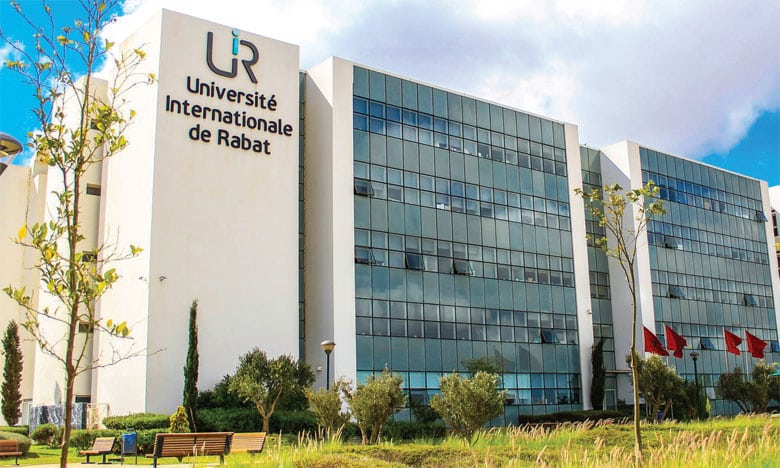
\includegraphics[width=0.7\textwidth]{img/imageuir.jpg}
    \caption{L'Université Internationale de Rabat}
    \label{fig:uir}
\end{figure}


% ---------------------------------------------------------------------
\subsection{L'École Supérieure d'Informatique et du Numérique (ESIN)}
\label{subsec:esin}

Le présent PFE est réalisé dans le cadre de la formation d'\textbf{ingénieur en informatique} dispensée par l'\textbf{École Supérieure d'Informatique et du Numérique (ESIN)}, composante de l'UIR. L'ESIN a pour mission de former des informaticiens hautement qualifiés et de mener des activités de recherche accompagnant le développement technologique et économique du Maroc.

La formation s'étend sur cinq ans : deux années de cycle préparatoire intégré, suivies de trois années de cycle ingénieur. La première année du cycle ingénieur constitue un tronc commun, et la deuxième année offre un choix de spécialisation entre : \textbf{Big Data}, \textbf{Ingénierie des systèmes d'information}, \textbf{Sécurité des systèmes d'information} et \textbf{Cloud Computing \& Virtualisation}.

Les objectifs pédagogiques du programme (PEO) visent à former des ingénieurs capables d'appliquer les principes de l'informatique dans un cadre professionnel, de déployer des fondements interdisciplinaires, et de résoudre de manière créative des problèmes au sein d'équipes pluridisciplinaires.

L'ESIN est née d'un partenariat académique entre l'UIR et l'Université de Nantes, et bénéficie de partenariats industriels avec des entreprises de premier plan, assurant ainsi une pédagogie axée sur l'insertion professionnelle et le rapprochement avec le monde socio-économique.


% =====================================================================
\section{Cadrage du projet de stage}
\label{sec:cadrage}

% ---------------------------------------------------------------------
\subsection{Sujet et périmètre de la mission}
\label{subsec:sujet}

Le sujet de ce PFE s'intitule : \og~\textbf{Développement d'une plateforme de migration de données basée sur l'IA pour l'amélioration et l'optimisation des processus d'intégration des données}~\fg{}.

Il s'inscrit dans le programme d'évolution d'ADMP visant à intégrer l'intelligence artificielle au cœur de la plateforme. Les objectifs stratégiques de cette intégration sont triples :

\begin{itemize}[leftmargin=*]
    \item \textbf{Rester un différenciateur réel} en matière de migration grâce à un moteur IA dédié (ADMP AI Engine).
    \item \textbf{Optimiser et accélérer} le temps nécessaire à la rédaction des spécifications de migration, et automatiser l'analyse des audits de données.
    \item \textbf{Créer un véritable assistant intelligent} pour les spécificateurs, réduisant la charge globale de travail.
\end{itemize}

Le périmètre de la mission couvre principalement la \textbf{génération du bundle Databricks}, un module central de la nouvelle architecture ADMP, dont les détails techniques seront présentés dans les chapitres~5 et~6. Ce module vise à automatiser la création des artefacts de migration en s'appuyant sur des technologies de traitement distribué (Apache Spark / Databricks) et d'intelligence artificielle générative.

% ---------------------------------------------------------------------
\subsection{Objectifs opérationnels et livrables attendus}
\label{subsec:objectifs}

Les objectifs opérationnels du PFE se déclinent comme suit :

\begin{itemize}[leftmargin=*]
    \item \textbf{Comprendre et maîtriser} la méthodologie ADMP et ses livrables (SDS, IDS, TDS, DS, RC, DP, TT, MS) à travers la formation Core ADMP Design School (CIDS).
    \item \textbf{Contribuer opérationnellement} aux projets de migration en cours, notamment en matière d'analyse de données, de validation de tickets et de rédaction de spécifications.
    \item \textbf{Concevoir et implémenter} le module de génération du bundle Databricks dans le cadre de l'évolution IA de la plateforme.
    \item \textbf{Tester et valider} la solution développée sur des cas réels de migration.
    \item \textbf{Documenter} l'ensemble du travail réalisé dans le présent rapport de PFE.
\end{itemize}

Ce travail s'inscrit dans la continuité des contributions précédentes de l'équipe : le PFE de Elharrioui Aymen portant sur la conception d'un agent intelligent basé sur RAG et l'architecture AppSync/GraphQL, et le PFE de Majbar Nizar portant sur le fine-tuning d'un LLM (Mistral 7B avec LoRA) pour la génération de règles de transformation.

% ---------------------------------------------------------------------
\subsection{Planning prévisionnel}
\label{subsec:planning}

Le stage se déroule sur une période de six mois, organisée en phases progressives, comme le résume le Tableau~\ref{tab:planning}.

\begin{table}[h!]
\centering
\caption{Planning prévisionnel du stage}
\label{tab:planning}
\begin{tabularx}{\textwidth}{l l X}
\toprule
\textbf{Phase} & \textbf{Période} & \textbf{Activités principales} \\
\midrule
Intégration \& Formation & Mois 1--2 & Onboarding, CIDS (2 semaines), découverte des outils et de la méthodologie ADMP \\
\addlinespace
Contribution opérationnelle & Mois 2--4 & Participation aux projets de migration, analyse de données, gestion de tickets, validation \\
\addlinespace
Conception \& Développement & Mois 3--5 & Conception et implémentation du module de génération du bundle Databricks \\
\addlinespace
Tests \& Validation & Mois 5--6 & Tests, évaluation, documentation, rédaction du rapport \\
\bottomrule
\end{tabularx}
\end{table}

\textit{Un diagramme de Gantt détaillé est présenté en annexe.}

% =====================================================================
\section{Organisation du rapport}
\label{sec:organisation}

Le présent rapport est structuré selon une logique narrative séquentielle, guidant le lecteur depuis la compréhension du problème jusqu'à la validation de la solution proposée :

\begin{itemize}[leftmargin=*]
    \item \textbf{Chapitre 2, Contexte et Problématique} : présente de manière générique les enjeux et défis de la migration de données, indépendamment de tout projet client, et formule la problématique de recherche.
    
    \item \textbf{Chapitre 3, État de l'Art} : explore les fondements théoriques de la migration, les solutions existantes sur le marché (outils ETL, services cloud), la plateforme ADMP dans son état actuel, les avancées de l'IA dans l'intégration de données, et identifie les limites et opportunités qui positionnent notre contribution.
    
    \item \textbf{Chapitre 4, Cadre Méthodologique et Gestion de Projet} : décrit l'organisation agile du travail, le cycle de vie des tickets, les processus de validation des données et les pratiques collaboratives de l'équipe.
    
    \item \textbf{Chapitre 5, Conception et Architecture de la Solution} : présente exclusivement les éléments nouveaux de notre contribution, l'architecture IA cible et le module de génération du bundle Databricks, en s'appuyant sur la description de l'existant fournie au chapitre~3.
    
    \item \textbf{Chapitre 6, Implémentation} : détaille la réalisation technique des modules, l'environnement de développement, et les difficultés rencontrées avec leurs solutions.
    
    \item \textbf{Chapitre 7, Résultats et Évaluation} : présente le protocole de test, les résultats obtenus et une discussion critique de la solution.
    
    \item \textbf{Chapitre 8, Conclusion et Perspectives} : synthétise les contributions, les compétences acquises et les pistes d'évolution futures.
\end{itemize}
% ============================================================
%  Chapitre 2 : Contexte et Problématique
%  Fichier : 05_context.tex
% ============================================================

\chapter{Contexte et Problématique}

La transformation numérique est devenue un impératif stratégique pour les
entreprises de toutes tailles et de tous secteurs. Selon IDC, les dépenses
mondiales en transformation digitale devraient atteindre près de
\textbf{4\,000 milliards USD d'ici 2027}, avec un taux de croissance annuel
composé (CAGR) de 16,2\,\%~\cite{integrate_io_stats}. Au cœur de cette
transformation se trouve un processus souvent sous-estimé mais fondamental :
la migration de données. Qu'il s'agisse de remplacer un système legacy par
une plateforme moderne, de consolider des bases de données après une
fusion-acquisition, d'adopter des solutions cloud pour gagner en agilité, ou
de préparer une infrastructure \textit{AI-ready} pour exploiter le potentiel
de l'intelligence artificielle, la migration constitue le socle invisible sur
lequel repose le succès --- ou l'échec --- de tout projet de modernisation.

Pourtant, la réalité est préoccupante : selon une analyse BCG portant sur
plus de 850 entreprises, seules \textbf{35\,\% des initiatives de
transformation digitale atteignent leurs objectifs}~\cite{integrate_io_stats}.
Le reste échoue ou livre des résultats en deçà des attentes, souvent à cause
de fondations de données fragiles. Ce chapitre dresse un panorama des enjeux
et des défis liés à la migration de données, avant de formuler la
problématique qui guidera l'ensemble de ce travail.

% ------------------------------------------------------------
\section{La migration de données : définition et enjeux}
% ------------------------------------------------------------

\subsection{Qu'est-ce qu'une migration de données ?}

La migration de données désigne le transfert structuré et planifié de données
d'un système source vers un système cible, en garantissant intégrité, qualité,
sécurité et conformité tout au long du processus. Ce processus repose sur le
triptyque \textbf{ETL} (\textit{Extract, Transform, Load})~\cite{microsoft_etl} :
extraction depuis le système source, transformation pour adapter les données au
modèle cible (nettoyage, standardisation, enrichissement, application des règles
métier), et chargement dans le nouveau système. Une variante moderne, l'approche
\textbf{ELT} (\textit{Extract, Load, Transform}), inverse les deux dernières
étapes en exploitant la puissance de calcul des entrepôts de données cloud
(Snowflake, BigQuery, Azure Synapse) pour effectuer les transformations après
le chargement~\cite{latentview2026, alphabyte_etl}.

\begin{figure}[H]
    \centering
    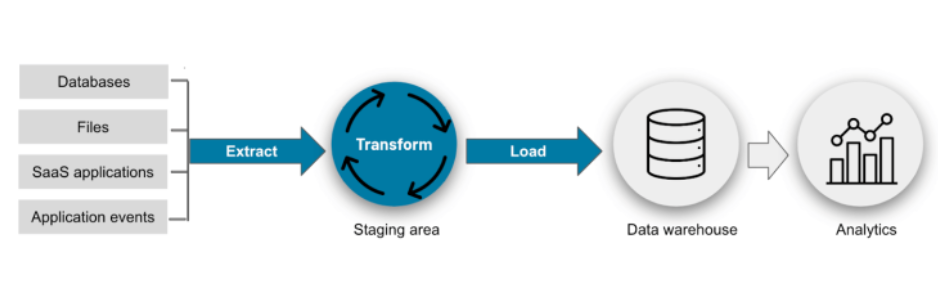
\includegraphics[width=0.85\linewidth]{img/ETL.png}
    \caption{Schéma du processus ETL classique --- extraction, transformation
    et chargement des données.}
    \label{fig:etl_schema}
\end{figure}

Il est important de distinguer la migration de données de concepts voisins :
l'\textbf{intégration continue} (synchronisation permanente entre systèmes
en temps réel), la \textbf{réplication} (copie à l'identique pour la haute
disponibilité) et l'\textbf{archivage} (déplacement de données historiques
vers un stockage de moindre coût). La migration se caractérise par son
caractère \textbf{ponctuel et planifié}, avec un périmètre défini, une
fenêtre d'exécution limitée et un objectif de basculement définitif vers
le système cible~\cite{cloudficient2025}.

Les projets de migration se déclinent en \textbf{cinq typologies
principales}~\cite{admp_core, latentview2026} :

\begin{itemize}
    \item \textbf{Re-platforming} --- Remplacement d'un système legacy par
    une plateforme moderne (Salesforce, SAP, Workday, Duck Creek). C'est le
    cas le plus fréquent dans le secteur de l'assurance et de la banque.

    \item \textbf{Consolidation post-fusion} --- Unification de bases de
    données hétérogènes suite à une fusion-acquisition, nécessitant la
    réconciliation de schémas, de référentiels et de règles métier
    divergents.

    \item \textbf{Migration cloud} --- Transfert des données et des
    workloads vers des plateformes cloud (AWS, Azure, GCP). En 2026,
    \textbf{94\,\% des entreprises} utilisent au moins un service cloud
    et \textbf{60\,\% des données d'entreprise} sont désormais stockées
    dans le cloud~\cite{medhacloud2026, datastackhub2026}.

    \item \textbf{Profiling et cleansing} --- Amélioration de la qualité
    des données (dédoublonnage, normalisation, enrichissement) avant
    réinjection dans le système existant ou un nouveau système.

    \item \textbf{Externalisation BPO} --- Transfert sécurisé de données
    vers un prestataire externe dans le cadre d'une externalisation de
    processus métier.
\end{itemize}

\subsection{Enjeux stratégiques pour les entreprises}

La migration de données est bien plus qu'un exercice technique : c'est un
enjeu stratégique à fort impact business dont les dimensions sont multiples.

\subsubsection{Un marché en croissance exponentielle}

Le marché mondial de la migration de données connaît une expansion
remarquable. Selon les estimations convergentes de plusieurs cabinets
d'analyse, il est évalué entre \textbf{15 et 21 milliards USD en 2025}
et devrait atteindre \textbf{36 à 48 milliards USD d'ici 2032--2035},
avec un CAGR oscillant entre 12 et 17\,\% selon les
périmètres~\cite{datamintel2026, reportsanddata2026, researchandmarkets2026,
fortunebi2026}. Le marché plus large des services de migration cloud
représente à lui seul \textbf{31,5 milliards USD en 2026}, avec un CAGR
de 22,4\,\%~\cite{medhacloud2026}.

\begin{figure}[H]
    \centering
    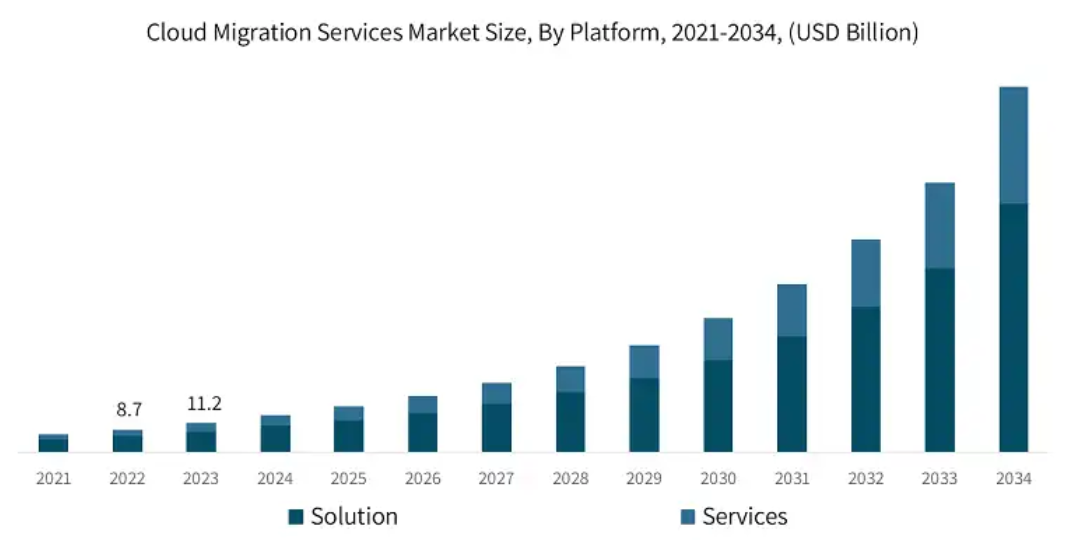
\includegraphics[width=0.85\linewidth]{img/migration_prev.png}
    \caption{Évolution du marché mondial de la migration de données
    (2024--2035), sources multiples.}
    \label{fig:market_growth}
\end{figure}

Cette croissance est portée par quatre forces motrices majeures identifiées
par Business Research Insights~\cite{bri2026} : l'\textbf{adoption du cloud}
(facteur cité par 65\,\% des organisations), la \textbf{croissance des volumes
de données} (58\,\%), les \textbf{initiatives de transformation digitale}
(62\,\%) et l'\textbf{adoption de l'IA et de l'automatisation} (54\,\%).

\subsubsection{Les dimensions stratégiques de la migration}

Tu peux la condenser ainsi :

Au-delà de la croissance du marché, plusieurs enjeux stratégiques rendent la migration des données essentielle. Elle garantit la continuité d’activité en limitant les risques de perte de données, assure la conformité réglementaire face aux exigences croissantes de protection des données, et représente un enjeu majeur de maîtrise des coûts dans les projets de modernisation IT. Elle constitue également une base indispensable pour les initiatives d’IA et d’analytique avancée, qui reposent sur des données fiables et bien gouvernées. Enfin, une migration réussie procure un avantage concurrentiel, en permettant aux entreprises d’exploiter leurs données plus rapidement et d’améliorer leur retour sur investissement.


% ------------------------------------------------------------
\section{Anatomie d'un projet de migration : les défis}
% ------------------------------------------------------------

Malgré son importance stratégique, la migration de données reste l'un des
processus les plus risqués du paysage IT. Les statistiques sont éloquentes :
selon Gartner, \textbf{83\,\% des projets de migration échouent ou dépassent
leur budget et leurs délais}~\cite{kaopiz2025, kanerika2025}. Le Bloor Group
rapporte des dépassements moyens de \textbf{30\,\% en coût et de 41\,\% en
délai}~\cite{vovance_medium}. Et selon les données Accenture les plus
récentes, seules \textbf{65\,\% des migrations sont livrées dans les temps
et le budget prévu}~\cite{medhacloud2026}. Six défis structurels expliquent
ces résultats.

\begin{figure}[H]
    \centering
    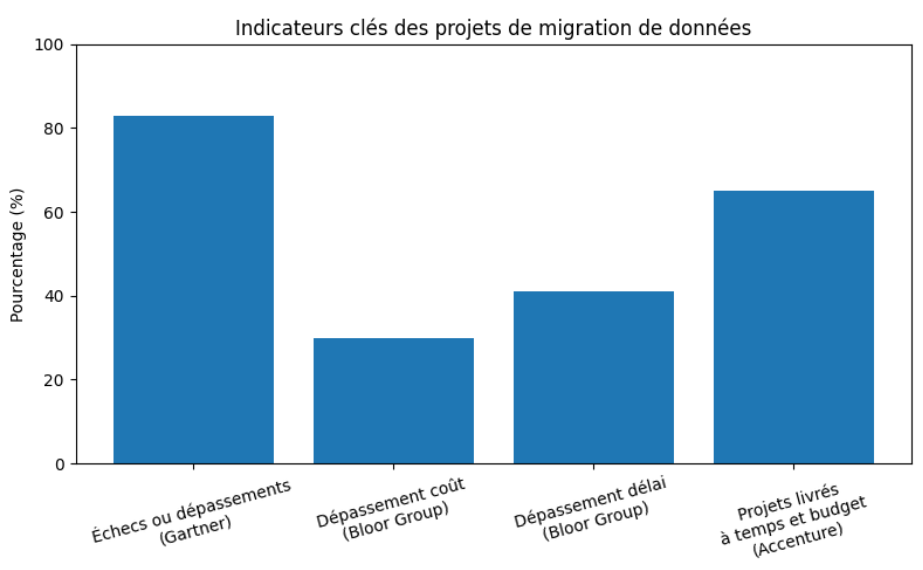
\includegraphics[width=0.85\linewidth]{img/graphe.png}
    \caption{les défis d'un projet de migration}
    \label{fig:market_growth}
\end{figure}

\subsection{Hétérogénéité des systèmes source et cible}

Le premier défi fondamental réside dans la disparité entre les systèmes
d'origine et de destination. Les données sources peuvent provenir de bases
relationnelles (Oracle, SQL Server, DB2), de fichiers plats (CSV, TXT), de
systèmes mainframe (VSAM, IMS), ou d'applications métier propriétaires,
chacun avec ses propres formats, encodages et conventions de
nommage~\cite{admp_presentation}. Le système cible, quant à lui, impose
son propre modèle de données, ses contraintes d'intégrité référentielle et
ses règles de validation.

Cette hétérogénéité génère des incompatibilités de schéma à l'origine de
\textbf{45\,\% des échecs de migration}~\cite{cloudficient2025}. La
réconciliation entre ces modèles divergents nécessite un travail minutieux
de mapping --- à la fois au niveau des tables (\textit{Table Mapping}) et
des champs (\textit{Data Mapping}) --- qui constitue l'un des exercices les
plus chronophages et les plus sujets à erreur. Un exemple révélateur : un
assureur majeur a vu 127\,000 polices des années 1940 migrées avec une date
d'émission en 2040, en raison d'un bug non documenté de format de dates dans
le système legacy~\cite{vovance_medium}.

\subsection{Volumétrie et performance}
La part des workloads d’entreprise déployés dans des environnements cloud ou edge devrait connaître une forte progression au cours des prochaines années. Selon Gartner, cette proportion passera de 52  en 2024 à 75  en 2028, soit une augmentation de 23 points en quatre ans. Cette évolution traduit l’accélération de la transformation numérique et entraîne des migrations de données de plus en plus massives. Les entreprises doivent ainsi gérer des volumes croissants de données tout en faisant face à des contraintes de bande passante, de latence et de disponibilité, ce qui accroît considérablement la complexité de la planification et de l’exécution des migrations.

\begin{figure}[H]
    \centering
    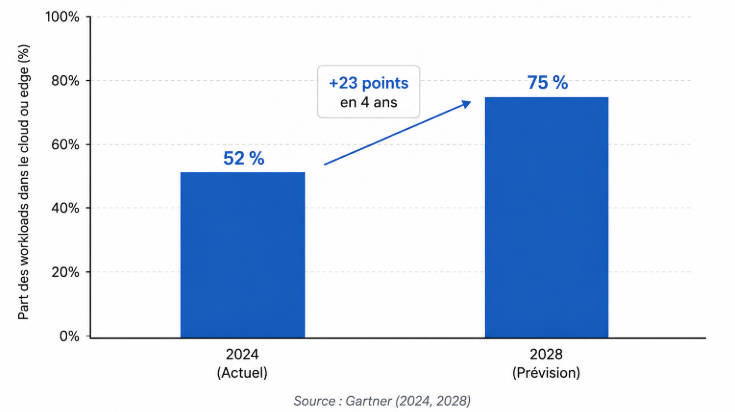
\includegraphics[width=0.85\linewidth]{img/graphe1.png}
    \caption{Evolution de la part des woekloads d'entreprise dans des environnements cloud ou edge}
    \label{fig:market_growth}
\end{figure}

~\cite{kaopiz2025}
~\cite{medhacloud2026}

\subsection{Qualité et intégrité des données}

La mauvaise qualité des données représente un risque financier et opérationnel majeur,
dont l'impact est particulièrement exacerbé lors des phases de migration.Ce phénomène engendre des coûts micro et macroéconomiques colossaux, tout en altérant structurellement la réussite des projets.

En contexte de migration, ces défaillances (données incomplètes, dupliquées ou corrompues) 
deviennent le principal facteur de dérive des projets. Elles se traduisent par des retards 
systématiques pour près de la moitié des organisations, provoquant par effet de cascade une explosion des budgets et un taux d'échec critique sur les délais de livraison.

~\cite{gartner_quality}
~\cite{forbes_bad_data}.
~\cite{alation_migration}. 
~\cite{montecarlo2025}.

\begin{figure}[H]
    \centering
    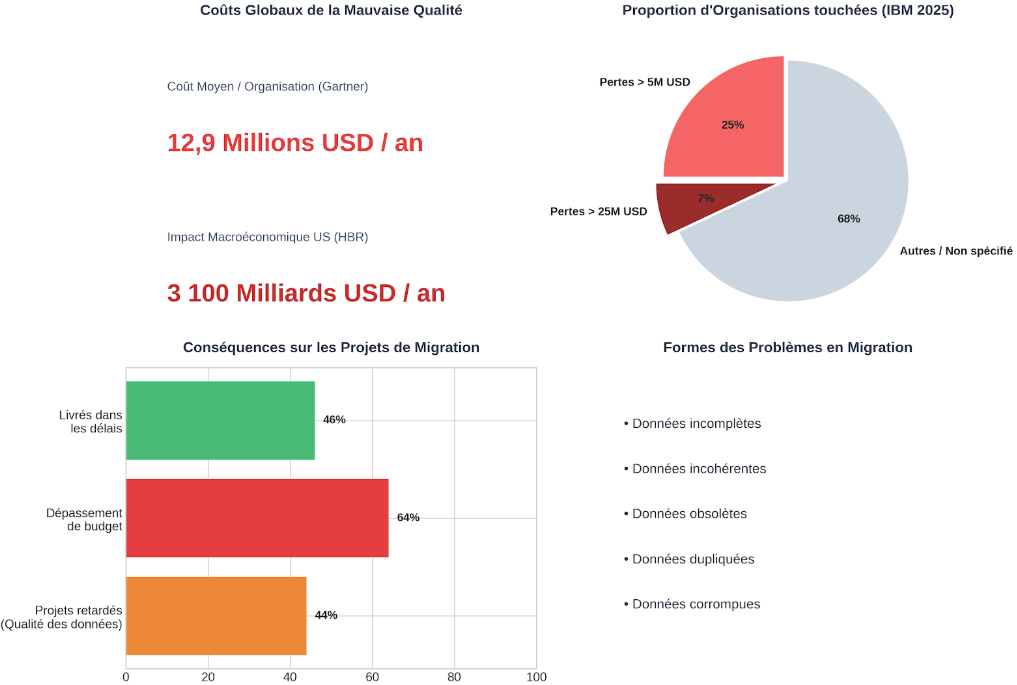
\includegraphics[width=0.85\linewidth]{img/impact_data_quality.png}
    \caption{L'impact de la mauvaise qualité des données}
    \label{fig:market_growth}
\end{figure}

\subsection{Complexité des règles de transformation}

La migration ne se limite pas à un simple transfert de données : elle
implique l'application de règles métier souvent complexes et mal
documentées. Parmi les défis typiques :

\begin{itemize}
    \item Relations \textbf{N:M} entre tables source et cible, nécessitant
    des mécanismes de dédoublonnage et de réconciliation.
    \item \textbf{Transcodification} entre référentiels source et cible
    (codes produits, statuts, identifiants).
    \item \textbf{Création conditionnelle} d'enregistrements selon des
    critères métier (périmètre fonctionnel, scope de migration).
    \item Gestion des \textbf{cas particuliers} et des données historiques
    (polices résiliées, bénéficiaires décédés, dossiers archivés).
    \item \textbf{Logique de fallback} lorsque des données source sont
    absentes ou invalides.
\end{itemize}

La formalisation de ces règles constitue l'un des postes les plus coûteux en
temps et en expertise, creusant le fossé entre spécifications fonctionnelles
et traduction technique. Comme le souligne Kanerika, les pipelines ETL
\textbf{encodent de la logique métier} : une seule règle mal traduite peut
corrompre des rapports financiers pendant des mois avant d'être
détectée~\cite{kanerika_etl}.

\subsection{Traçabilité et auditabilité}

Dans un environnement réglementaire de plus en plus exigeant,
\textbf{34\,\% des organisations rapportent des lacunes de conformité
durant la migration} et \textbf{38\,\% déclarent que la préparation aux
audits est difficile}~\cite{gitnux_cloud, admp_overview}. Les outils ETL
traditionnels, souvent qualifiés de \textbf{boîtes noires} (\textit{black
boxes}), rendent cette traçabilité particulièrement ardue : les
transformations appliquées aux données sont opaques, les versions des règles
difficiles à suivre, et la réconciliation entre données source et cible
laborieuse.

Cette opacité est d'autant plus problématique que les organisations doivent
aujourd'hui garantir une \textbf{traçabilité de bout en bout}
(\textit{data lineage}) de chaque donnée migrée, depuis son extraction du
système source jusqu'à son chargement dans le système cible, en passant par
chaque transformation appliquée. Les régulateurs exigent de pouvoir auditer
chaque étape du processus, ce qui impose des mécanismes de versionnement,
de journalisation et de reporting que les approches traditionnelles peinent
à fournir.

\subsection{Coordination IT / Business et gestion du changement}

La migration se situe à l'intersection des équipes techniques et métier,
générant une véritable \textbf{barrière linguistique} entre ces deux
mondes. Les spécificateurs fonctionnels décrivent des règles métier en
langage naturel, tandis que les développeurs doivent les traduire en code
technique --- un processus source d'erreurs d'interprétation, de cycles de
validation longs et de frustrations mutuelles.

Les statistiques confirment l'ampleur du problème : \textbf{70\,\% des
migrations échouent en partie à cause d'une mauvaise gestion du changement},
et \textbf{80\,\% des organisations citent le manque d'expertise interne
comme principal frein}~\cite{worldmetrics2025, wifitalents2025}. La pénurie
de talents IT est critique : selon les projections, jusqu'à \textbf{90\,\%
des organisations feront face à des pénuries de compétences IT}, avec des
pertes estimées à \textbf{5\,500 milliards USD d'ici 2026} liées à ces
lacunes~\cite{integrate_io_stats}.

De plus, la résistance au changement des utilisateurs finaux, combinée à
une formation insuffisante, compromet l'adoption du nouveau système même
lorsque la migration technique est réussie. Dans le domaine des ERP, par
exemple, \textbf{29\,\% des utilisateurs} déclarent ne pas comprendre
comment utiliser le nouveau système après migration~\cite{godlan_erp}.

\begin{table}[H]
\centering
\caption{Synthèse des principaux défis d'un projet de migration de données.}
\label{tab:defis_migration}
\begin{tabular}{lll}
\hline
\textbf{Défi} & \textbf{Impact principal} & \textbf{Statistique clé} \\
\hline
Hétérogénéité des systèmes    & Incompatibilités, corruption   & 45\,\% des échecs \\
Volumétrie et performance     & Dépassements de délais         & 181 ZB créés en 2025 \\
Qualité des données           & Surcoûts, reprises             & 12,9 M\$/an (Gartner) \\
Complexité des transformations & Écart design--build           & 30--50\,\% du budget IT \\
Traçabilité et auditabilité   & Non-conformité                 & 34\,\% de lacunes \\
Coordination IT / Business    & Retards, malentendus           & 70\,\% liés au change management \\
\hline
\end{tabular}
\end{table}

% ------------------------------------------------------------
\section{L'émergence de l'IA dans la migration de données}
% ------------------------------------------------------------

Face à ces défis, l'intelligence artificielle émerge comme un levier
transformateur. Selon Business Research Insights: 

\begin{figure}[H]
    \centering
    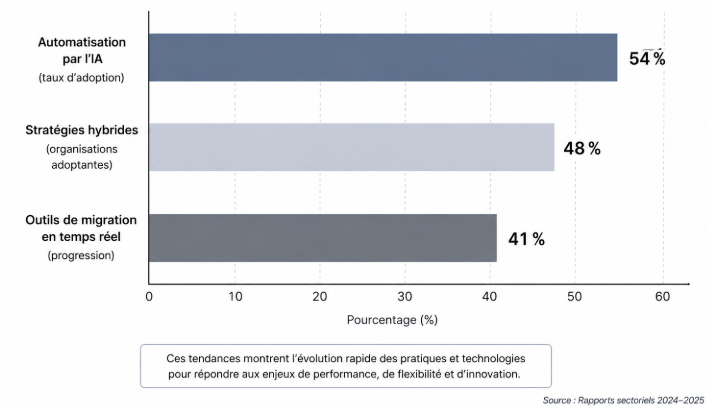
\includegraphics[width=0.85\linewidth]{img/graphe2.png}
    \caption{Tendances clés dans les solutions de migration}
    \label{fig:market_growth}
\end{figure}

~\cite{bri2026}.

L'IA transforme la migration de données à plusieurs niveaux~\cite{buzzclan2026,
ispirer_ai} :

\begin{itemize}
    \item \textbf{Data profiling intelligent} : Les algorithmes de ML
    détectent automatiquement les anomalies, les valeurs nulles dans des
    colonnes inattendues, les formats de dates non documentés et les
    enregistrements orphelins, là où le profiling manuel procède par
    échantillonnage statistique.

    \item \textbf{Mapping automatisé} : L'IA analyse les systèmes source
    et cible pour créer des correspondances de schéma sans intervention
    manuelle, réduisant drastiquement le temps de mapping.

    \item \textbf{Validation prédictive} : Les modèles de ML identifient
    les goulots d'étranglement et les risques de défaillance avant qu'ils
    ne surviennent, permettant une approche proactive plutôt que réactive.

    \item \textbf{Génération de règles de transformation} : Les LLM
    (\textit{Large Language Models}) peuvent générer des règles de
    transformation à partir de spécifications en langage naturel, comblant
    le fossé entre spécificateurs fonctionnels et développeurs.

    \item \textbf{Optimisation des coûts} : L'IA identifie les données
    redondantes ou non critiques, réduisant les volumes à migrer et les
    coûts de stockage associés.
\end{itemize}

Selon les projections, l'IA augmentée en gestion de données pourrait
\textbf{réduire de 45\,\% le besoin en spécialistes IT} pour les tâches
routinières de migration~\cite{ispirer_ai}. Cependant, malgré ces promesses,
l'adoption reste limitée : seulement \textbf{35\,\% des entreprises}
utilisent actuellement des plateformes de migration augmentées par
l'IA~\cite{reanin2025}, et \textbf{74\,\% des entreprises peinent à
passer à l'échelle} avec leurs initiatives IA~\cite{integrate_io_stats}.
Cet écart entre potentiel et adoption constitue une opportunité majeure
pour les acteurs innovants du marché.

% ------------------------------------------------------------
\section{Formulation de la problématique}
% ------------------------------------------------------------

L'analyse précédente fait émerger trois lacunes structurelles communes aux
approches actuelles de migration, que nous synthétisons dans la figure
ci-dessous :

\begin{itemize}
 \item \textbf{Le fossé Design-Build} : un décalage significatif persiste
entre la rédaction des spécifications fonctionnelles et leur implémentation
technique. Les spécificateurs décrivent les règles métier en langage naturel,
les développeurs les traduisent en code, et entre les deux, la perte de
fidélité est inévitable~\cite{admp_overview}. Ce fossé ne se limite d'ailleurs
pas au code applicatif : la traduction doit aboutir à des artefacts
d'intégration réellement exécutables sur les plateformes cloud d'orchestration
(par exemple des pipelines Azure Data Factory), ce qui ajoute une couche
d'expertise technique et autant de sources d'erreur.

    \item \textbf{L'opacité des processus} : les outils ETL traditionnels
    fonctionnent comme des boîtes noires, rendant difficile la validation
    fonctionnelle, l'auditabilité et la réconciliation par les équipes non
    techniques. Dans un contexte réglementaire où 172 pays disposent de lois
    sur la protection des données~\cite{stationx_privacy}, cette opacité
    n'est plus acceptable.

    \item \textbf{L'absence d'intelligence artificielle} : les processus de
    migration restent largement manuels et réactifs, alors que l'IA offre
    des possibilités transformatrices en matière d'automatisation, de
    validation prédictive et de génération intelligente de règles.
    Seulement \textbf{35\,\% des entreprises} utilisent des plateformes
    augmentées par l'IA~\cite{reanin2025}, laissant un immense potentiel
    inexploité.
\end{itemize}

Ces constats, croisés avec les réalités du terrain observées dans le cadre
de ce stage au sein de l'équipe ADMP d'Accenture, amènent à formuler la
problématique suivante :

\begin{quote}
\textit{Comment concevoir et implémenter une plateforme de migration de
données intégrant l'intelligence artificielle pour automatiser et optimiser
les processus d'intégration, réduire le fossé entre la conception
fonctionnelle et l'exécution technique, et améliorer la qualité, la
traçabilité et l'efficience globale du processus de migration ?}
\end{quote}

Cette problématique sera explorée à travers l'état de l'art (chapitre
suivant), qui examinera les solutions existantes  y compris la plateforme
ADMP et son architecture actuelle  et les avancées de l'IA dans ce
domaine, avant de présenter notre contribution : le développement d'un
module de génération automatisée intégré à l'évolution IA de la plateforme
ADMP.
% =====================================================================
% ÉTAT DE L'ART
% =====================================================================
\chapter{État de l'Art}
\section{État de l'Art}
\label{sec:etat-art}

Le chapitre précédent a mis en lumière les défis structurels de la migration de données et formulé la problématique centrale de ce travail. Le présent chapitre explore l'état de l'art scientifique et technologique afin d'identifier les fondements, les solutions existantes, et les opportunités d'amélioration qui positionnent notre contribution. Nous commençons par les fondements théoriques, passons en revue les solutions du marché, décrivons en profondeur la plateforme ADMP dans son état actuel, explorons les avancées de l'intelligence artificielle appliquées au domaine, avant d'analyser les limites de l'existant et de formuler notre positionnement.

% =====================================================================
\subsection{Fondements théoriques}
\label{subsec:fondements}

% ---------------------------------------------------------------------
\subsubsection{Le paradigme ETL / ELT : principes et évolution}
\label{subsubsec:etl-elt}

Le paradigme \textbf{ETL (Extract, Transform, Load)} constitue depuis plusieurs décennies le socle fondamental de toute opération d'intégration de données. Il décrit un processus en trois phases séquentielles : l'\textbf{extraction} des données depuis les systèmes sources, leur \textbf{transformation} dans une zone intermédiaire (staging) pour les adapter au modèle cible, puis leur \textbf{chargement} dans le système de destination. Ce paradigme a été le pilier de l'ère du data warehousing classique, où les ressources de calcul étaient limitées et coûteuses, imposant un pré-traitement rigoureux des données avant leur insertion dans l'entrepôt.

Avec l'avènement du cloud computing et des entrepôts de données modernes (Snowflake, BigQuery, Amazon Redshift), un paradigme alternatif a émergé : l'\textbf{ELT (Extract, Load, Transform)}. Dans cette approche, les données brutes sont d'abord chargées dans le système cible, puis transformées directement en exploitant la puissance de calcul élastique de l'infrastructure cloud. L'ELT offre une flexibilité analytique accrue, une meilleure utilisation des ressources et un time-to-insight réduit, tout en posant de nouveaux défis en matière de gouvernance et de gestion technique.

\begin{figure}[H]
    \centering
    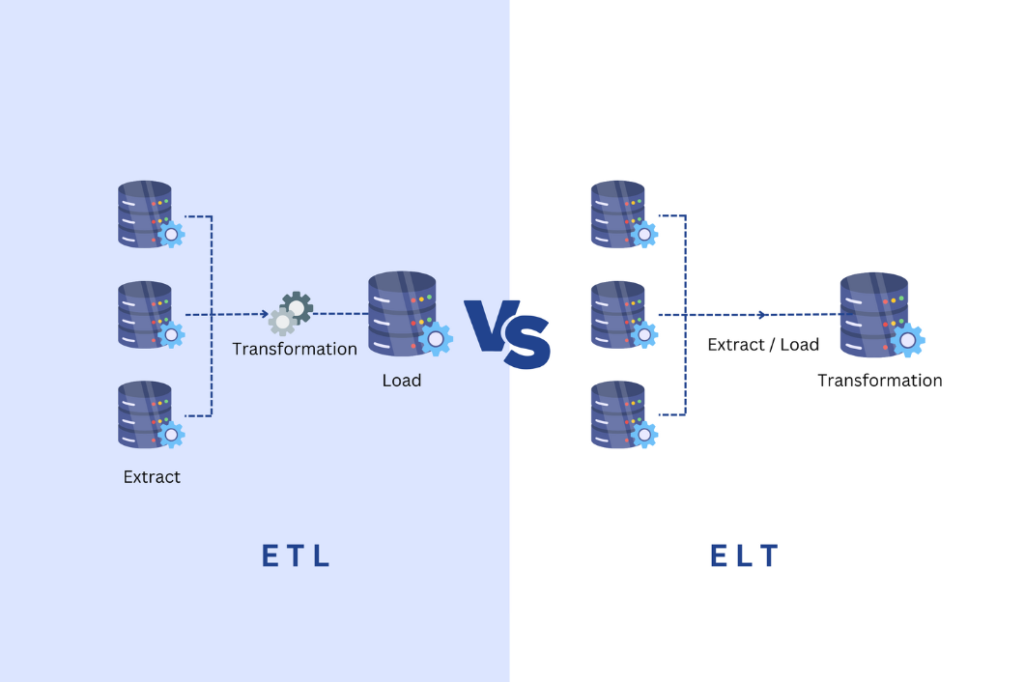
\includegraphics[width=0.9\textwidth]{img/ETL_VS_ELT.png}
    \caption{Comparaison des paradigmes ETL et ELT}
    \label{fig:etl-vs-elt}
\end{figure}

L'évolution de l'ETL vers l'ELT ne se résume pas à une simple réorganisation des étapes : elle reflète un changement fondamental dans la philosophie de gestion des données. Comme le souligne Vanga (2024) dans son étude publiée dans l'\textit{International Journal for Multidisciplinary Research}, cette transition est catalysée par la croissance exponentielle des volumes de données, la prolifération des sources hétérogènes, et les exigences d'analyse en temps réel. Les architectures modernes tendent vers des modèles hybrides combinant les forces des deux approches, avec l'émergence de concepts tels que le \textbf{zero-ETL} et le \textbf{data mesh} qui promettent de réduire encore la complexité des pipelines de données.
Le Tableau~\ref{tab:etl-elt-comparison} présente une comparaison synthétique des deux paradigmes.

\begin{table}[H]
\centering

\begin{tabularx}{\textwidth}{lXX}
\toprule
\textbf{Critère} & \textbf{ETL} & \textbf{ELT} \\
\midrule
Transformation & Avant le chargement (staging) & Après le chargement (in-warehouse) \\
\addlinespace
Infrastructure & On-premise, ressources limitées & Cloud-native, calcul élastique \\
\addlinespace
Flexibilité & Schéma rigide, pré-défini & Schéma flexible, late-binding \\
\addlinespace
Vitesse & Plus lent sur grands volumes & Plus rapide (puissance cloud) \\
\addlinespace
Gouvernance & Contrôle pré-chargement & Nécessite gouvernance SQL forte \\
\addlinespace
Outils typiques & Informatica, Talend, SSIS & dbt, Snowflake, BigQuery \\
\bottomrule
\end{tabularx}
\caption{Comparaison entre ETL et ELT}
\label{tab:etl-elt-comparison}
\end{table}

% ---------------------------------------------------------------------
\subsubsection{Modélisation des données}
\label{subsubsec:modelisation}

La réussite d'un projet de migration repose en grande partie sur la maîtrise des modèles de données source et cible. Trois approches principales de modélisation coexistent dans l'écosystème :

\begin{itemize}[leftmargin=*]
    \item \textbf{Le modèle relationnel}, fondé sur les travaux de Codd (1970), organise les données en tables liées par des clés primaires et étrangères. Il reste le standard dominant dans les systèmes transactionnels (OLTP) et les plateformes CRM comme Salesforce.
    
    \item \textbf{Le modèle dimensionnel}, popularisé par Kimball, structure les données autour de tables de faits et de dimensions, optimisées pour l'analyse (OLAP). Il est au cœur des entrepôts de données classiques.
    
    \item \textbf{Le modèle orienté objet}, qui encapsule données et comportements dans des objets liés par héritage et composition, est utilisé dans les systèmes modernes et les plateformes cloud-native. Comme le détaille la formation CIDS d'ADMP, \og~\textit{an object-oriented data model consists of basic concepts: Object, Object identifier, Attributes, Methods, Class, Class hierarchy, and Inheritance}~\fg{}.
\end{itemize}

La compréhension de ces modèles est essentielle pour le Data Analyst qui doit établir les correspondances (mappings) entre le système source et le système cible, en tenant compte des différences structurelles, des contraintes d'intégrité et des relations entre entités.

% ---------------------------------------------------------------------
\subsubsection{Qualité des données : métriques et frameworks}
\label{subsubsec:qualite-donnees}

La qualité des données est un facteur déterminant du succès de toute migration. Le concept de dimensions de qualité des données a été formalisé en 1996 par les professeurs Richard Y. Wang et Diane M. Strong dans leur article fondateur \og~\textit{Beyond Accuracy: What Data Quality Means to Data Consumers}~\fg{}. Depuis, le framework DAMA-DMBOK a standardisé \textbf{six dimensions fondamentales} universellement adoptées, présentées dans le Tableau~\ref{tab:data-quality}.

\begin{table}[H]
\centering

\begin{tabularx}{\textwidth}{lXX}
\toprule
\textbf{Dimension} & \textbf{Description} & \textbf{Exemple d'impact en migration} \\
\midrule
Exactitude & Les données reflètent-elles fidèlement la réalité ? & Adresse client erronée → livraison échouée \\
\addlinespace
Complétude & Tous les champs requis sont-ils renseignés ? & Champ obligatoire vide → rejet au chargement \\
\addlinespace
Cohérence & Les données sont-elles uniformes entre systèmes ? & Prix différent entre web et mobile \\
\addlinespace
Fraîcheur & Les données sont-elles disponibles à temps ? & Données obsolètes → décisions erronées \\
\addlinespace
Validité & Les données respectent-elles les formats et règles ? & Date \og~30 février~\fg{} → rejet de validation \\
\addlinespace
Unicité & Pas de doublons ? & Doublons clients → métriques faussées \\
\bottomrule
\end{tabularx}
\caption{Dimensions de la qualité des données et impact en migration}
\label{tab:data-quality}
\end{table}

Le coût de la non-qualité est considérable : selon Gartner (2023), la mauvaise qualité des données coûte en moyenne \textbf{12,9 millions de dollars par an} aux organisations. Dans le contexte spécifique de la migration, la mise en place de contrôles de qualité automatisés (profiling, validation pré-chargement, réconciliation post-chargement) est donc un prérequis incontournable.

\begin{figure}[H]
    \centering
    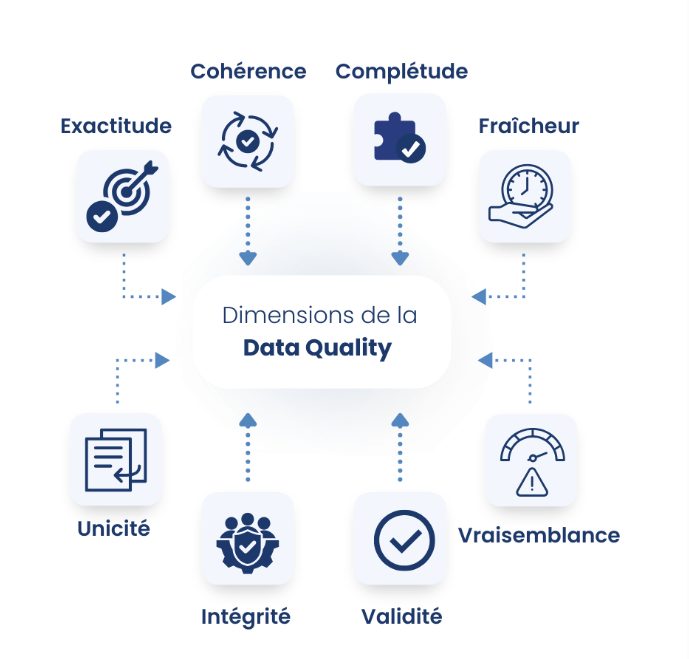
\includegraphics[width=0.7\textwidth]{img/Qualité de data.png}
    \caption{Les dimensions de la qualité des données }
    \label{fig:data-quality}
\end{figure}

% ---------------------------------------------------------------------
\subsubsection{Gouvernance des données et conformité}
\label{subsubsec:gouvernance}

La gouvernance des données établit les politiques, processus et responsabilités qui encadrent la gestion des données tout au long de leur cycle de vie. Dans le contexte de la migration, elle revêt une importance critique pour trois raisons :

Premièrement, la \textbf{traçabilité des données} (\textit{data lineage}), la capacité à retracer le parcours complet d'une donnée depuis son origine jusqu'à sa destination, en passant par chaque transformation, est devenue une exigence réglementaire explicite. Le RGPD (Article 30) impose aux organisations de maintenir des registres des activités de traitement, incluant la classification des données, le suivi de la qualité, et les politiques de rétention.

Deuxièmement, le \textbf{principe de responsabilité} (\textit{accountability}, Article 5(2) du RGPD) exige que les organisations puissent \textbf{démontrer}, et non simplement affirmer, leur conformité, à travers des politiques documentées, des rôles définis, des contrôles techniques et des traces d'audit.

Troisièmement, les réglementations émergentes comme l'\textbf{EU AI Act} ajoutent une couche supplémentaire de complexité : les organisations utilisant l'IA dans leurs processus de migration doivent documenter de manière exhaustive les flux de données, avec des amendes pouvant atteindre \textbf{7,5 à 35 millions d'euros} en cas de non-conformité.

L'intégration du data lineage dans le cadre de gouvernance offre des avantages concrets : amélioration de la redevabilité, support au troubleshooting, analyse d'impact proactive lors des mises à jour, et simplification des audits de conformité.

\begin{figure}[H]
    \centering
    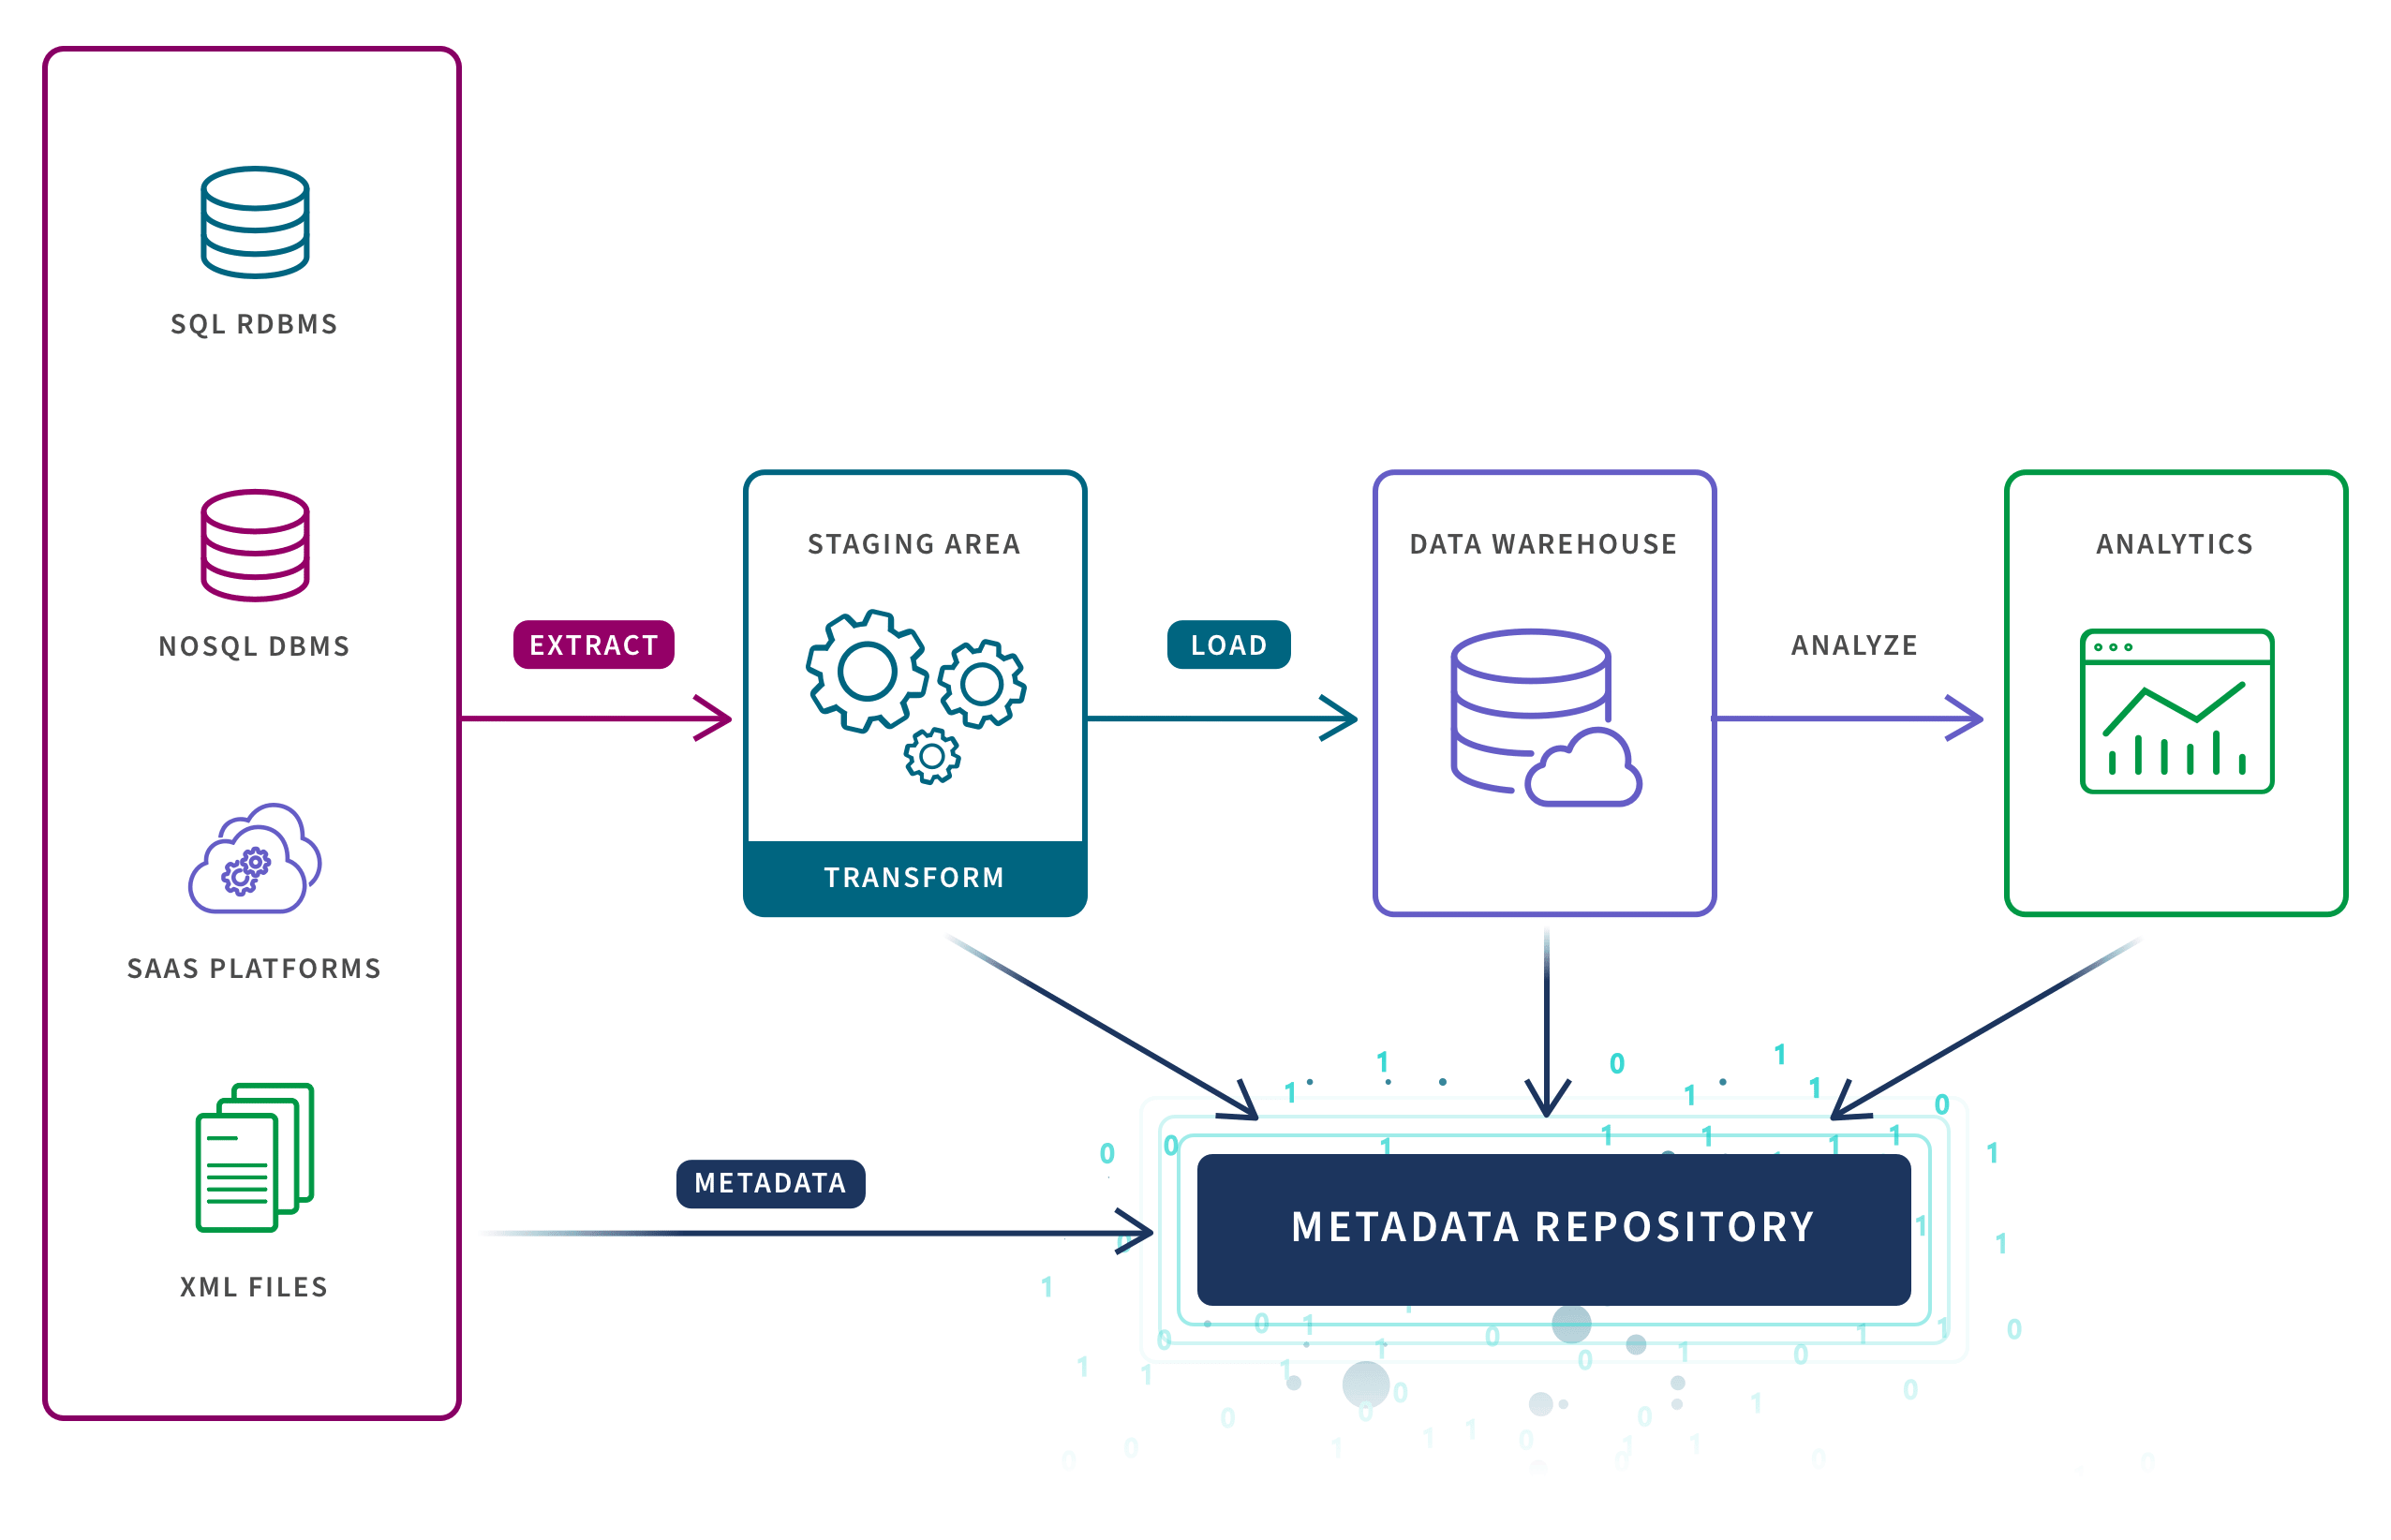
\includegraphics[width=0.85\textwidth]{img/data_lineage.png}
    \caption{Exemple de traçabilité des données (Data Lineage)}
    \label{fig:data-lineage}
\end{figure}

% =====================================================================
\subsection{Solutions existantes sur le marché}
\label{subsec:solutions-marche}

% ---------------------------------------------------------------------
\subsubsection{Outils ETL traditionnels}
\label{subsubsec:etl-traditionnels}

Le marché des outils ETL traditionnels est dominé par trois acteurs majeurs, chacun avec ses forces et ses limites :

\textbf{Informatica PowerCenter} est considéré comme la référence enterprise-grade. Il offre une large connectivité (Oracle, DB2, Teradata, NoSQL), un profilage automatique des données, et des mécanismes robustes de gestion des erreurs. Cependant, son coût de licence élevé, sa courbe d'apprentissage abrupte et son interface vieillissante limitent son accessibilité.

\textbf{Talend} propose une approche open-source (Talend Open Studio) complétée par une édition enterprise. Basé sur Java, il offre plus de 900 connecteurs, un support natif du Big Data (Hadoop, Spark), et une interface drag-and-drop accessible. Il constitue un choix privilégié pour les organisations cherchant flexibilité et maîtrise des coûts.

\textbf{SSIS (SQL Server Integration Services)} de Microsoft est intégré à SQL Server sans coût de licence additionnel. Performant dans les environnements Microsoft-centric, il souffre néanmoins d'un support limité pour les systèmes non-Microsoft et d'une scalabilité restreinte en environnements hétérogènes.

Le Tableau~\ref{tab:etl-tools-comparison} présente une comparaison détaillée de ces trois outils.

\begin{table}[H]
\centering
\caption{Comparaison des outils ETL traditionnels}
\label{tab:etl-tools-comparison}
\begin{tabularx}{\textwidth}{lXXX}
\toprule
\textbf{Critère} & \textbf{Informatica} & \textbf{Talend} & \textbf{SSIS} \\
\midrule
Type & Propriétaire & Open-source + Enterprise & Propriétaire (inclus SQL Server) \\
\addlinespace
Coût & Élevé & Gratuit (OS) / Modéré (Ent.) & Inclus avec SQL Server \\
\addlinespace
Cloud & Fort (IICS) & Excellent (cloud-native) & Limité (via ADF) \\
\addlinespace
Big Data & Add-ons requis & Support natif (Spark, Hadoop) & Support basique \\
\addlinespace
Connectivité & Très large & 900+ connecteurs & Fort en Microsoft \\
\addlinespace
Courbe d'apprentissage & Raide & Modérée & Modérée \\
\bottomrule
\end{tabularx}
\end{table}

% ---------------------------------------------------------------------
\subsubsection{Services cloud natifs}
\label{subsubsec:cloud-natifs}

L'essor du cloud a donné naissance à des services d'intégration de données entièrement managés :

\textbf{AWS Glue} est un service ETL serverless basé sur Apache Spark, intégré à l'écosystème AWS (S3, Redshift, Athena). Il propose un Data Catalog automatisé, le support batch et streaming, et un studio visuel de développement de pipelines.

\textbf{Azure Data Factory (ADF)} de Microsoft offre plus de 90 connecteurs natifs, des Data Flows Spark pour les transformations no-code, et un runtime d'intégration hybride permettant de connecter données on-premise et cloud. Son intégration avec Azure Synapse, Databricks et Power BI en fait un choix naturel pour les organisations dans l'écosystème Microsoft.

\textbf{Google Cloud Dataflow}, basé sur Apache Beam, se distingue par son modèle unifié batch/streaming et sa facturation à la seconde. Il excelle dans le traitement en temps réel et les workloads analytiques avancés.

Le Tableau~\ref{tab:cloud-services-comparison} compare ces trois services cloud.

\begin{table}[H]
\centering
\caption{Comparaison des services cloud natifs}
\label{tab:cloud-services-comparison}
\begin{tabularx}{\textwidth}{lXXX}
\toprule
\textbf{Critère} & \textbf{AWS Glue} & \textbf{Azure Data Factory} & \textbf{GCP Dataflow} \\
\midrule
Moteur & Apache Spark & Spark (Data Flows) & Apache Beam \\
\addlinespace
Modèle & Serverless & Serverless + IR & Serverless \\
\addlinespace
Connecteurs & 70+ & 90+ & Google Cloud natif \\
\addlinespace
Streaming & Oui (Kinesis, MSK) & Limité & Excellent (Pub/Sub) \\
\addlinespace
Coût/TB batch & $\sim$1,84 & $\sim$1,42 & $\sim$2,11 \\
\addlinespace
Latence streaming p99 & $\sim$120ms & $\sim$148ms & $\sim$89ms \\
\bottomrule
\end{tabularx}
\end{table}

% ---------------------------------------------------------------------
\subsubsection{Approches ad hoc / scripts custom}
\label{subsubsec:scripts-custom}

De nombreuses organisations développent encore des scripts ad hoc (SQL, Python, Shell) pour gérer leurs migrations. Cette approche offre une flexibilité maximale et un coût initial faible, mais présente des limites critiques : absence de standardisation, aucune traçabilité intrinsèque, dépendance aux développeurs individuels, maintenance difficile, et risque élevé d'erreurs sur les projets à grande échelle.

% ---------------------------------------------------------------------
\subsubsection{Analyse comparative et limites communes}
\label{subsubsec:limites-communes}

Malgré leurs différences, toutes ces solutions partagent des limitations structurelles communes :

\begin{itemize}[leftmargin=*]
    \item \textbf{Le fossé Design-Build} : dans chaque cas, les spécifications fonctionnelles doivent être traduites manuellement en code exécutable par une équipe technique, créant un risque permanent de décalage entre le design et l'implémentation.
    
    \item \textbf{Effet boîte noire} : les moteurs ETL traditionnels ne permettent pas aux équipes fonctionnelles de vérifier directement que le code implémenté correspond aux spécifications validées.
    
    \item \textbf{Absence de couche métier} : les services cloud natifs sont performants pour le transport de données, mais manquent de la couche fonctionnelle nécessaire pour gérer les règles de transformation complexes, les Key Decisions, et la validation métier itérative.
    
    \item \textbf{Coûts cachés} : licences logicielles, infrastructure dédiée, main-d'œuvre technique spécialisée, et coûts de maintenance s'accumulent au fil du projet.
\end{itemize}

C'est dans ce contexte que la plateforme ADMP se positionne comme une réponse industrielle visant à combler ces lacunes.

% =====================================================================
\subsection{La plateforme ADMP : état actuel}
\label{subsec:admp-actuel}

% ---------------------------------------------------------------------
\subsubsection{Envergure mondiale et chiffres clés}
\label{subsubsec:admp-envergure}

\begin{figure}[H]
    \centering
    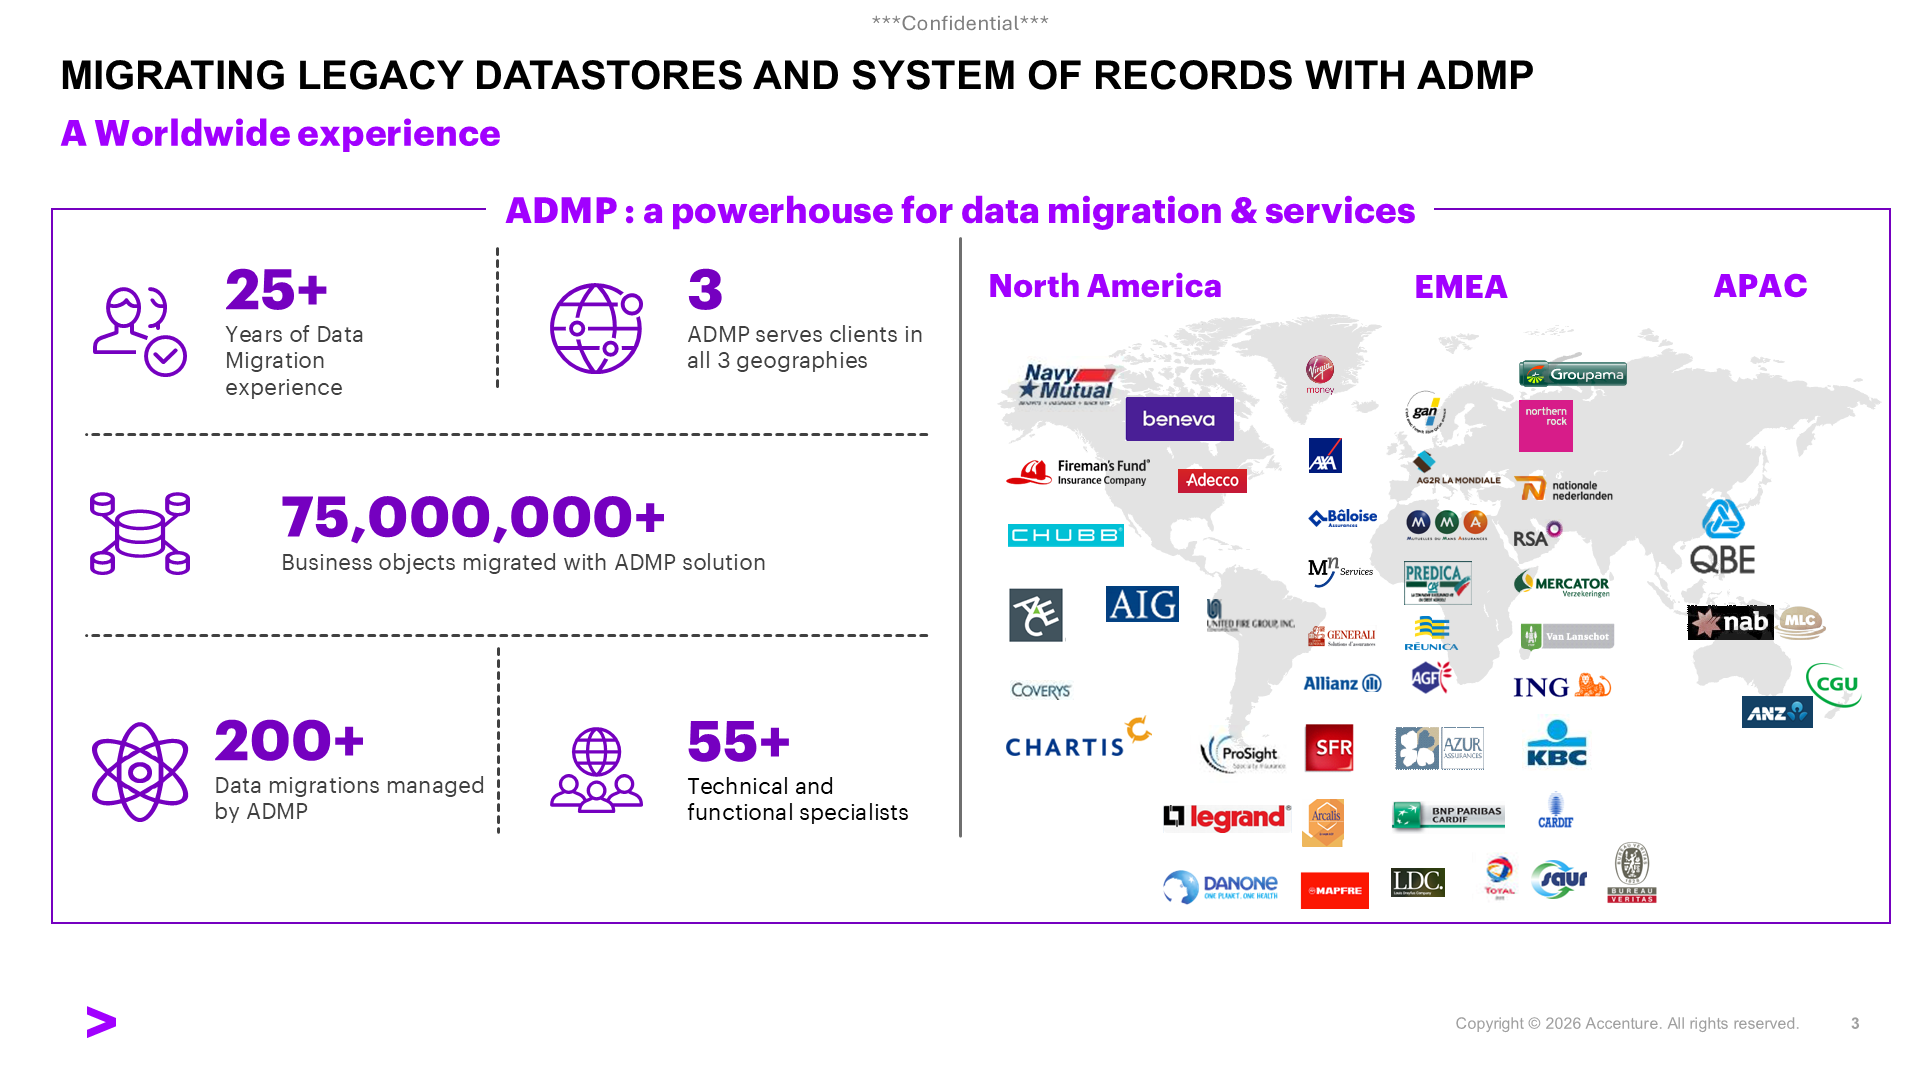
\includegraphics[width=0.85\textwidth]{img/admp_worldwide.png}
    \caption{Envergure mondiale de la plateforme ADMP : chiffres clés et 3 géographies}
    \label{fig:admp-worldwide}
\end{figure}

L'\textbf{Accenture Data Migration Platform (ADMP)} est une solution propriétaire d'Accenture dédiée à la migration de données d'entreprise à grande échelle. Forte de plus de \textbf{25 ans d'expérience}, la plateforme a accompagné plus de \textbf{200 projets de migration} à travers le monde, avec plus de \textbf{75 millions d'objets métier migrés} par une équipe de plus de \textbf{55 spécialistes} techniques et fonctionnels. La plateforme intervient dans \textbf{3 géographies} : North America, APAC et EMEA, positionnant ADMP comme \og~\textit{a powerhouse for data migration \& services}~\fg{}.

% ---------------------------------------------------------------------
\subsubsection{Quatre piliers de valeur}
\label{subsubsec:admp-piliers}

\begin{figure}[H]
    \centering
    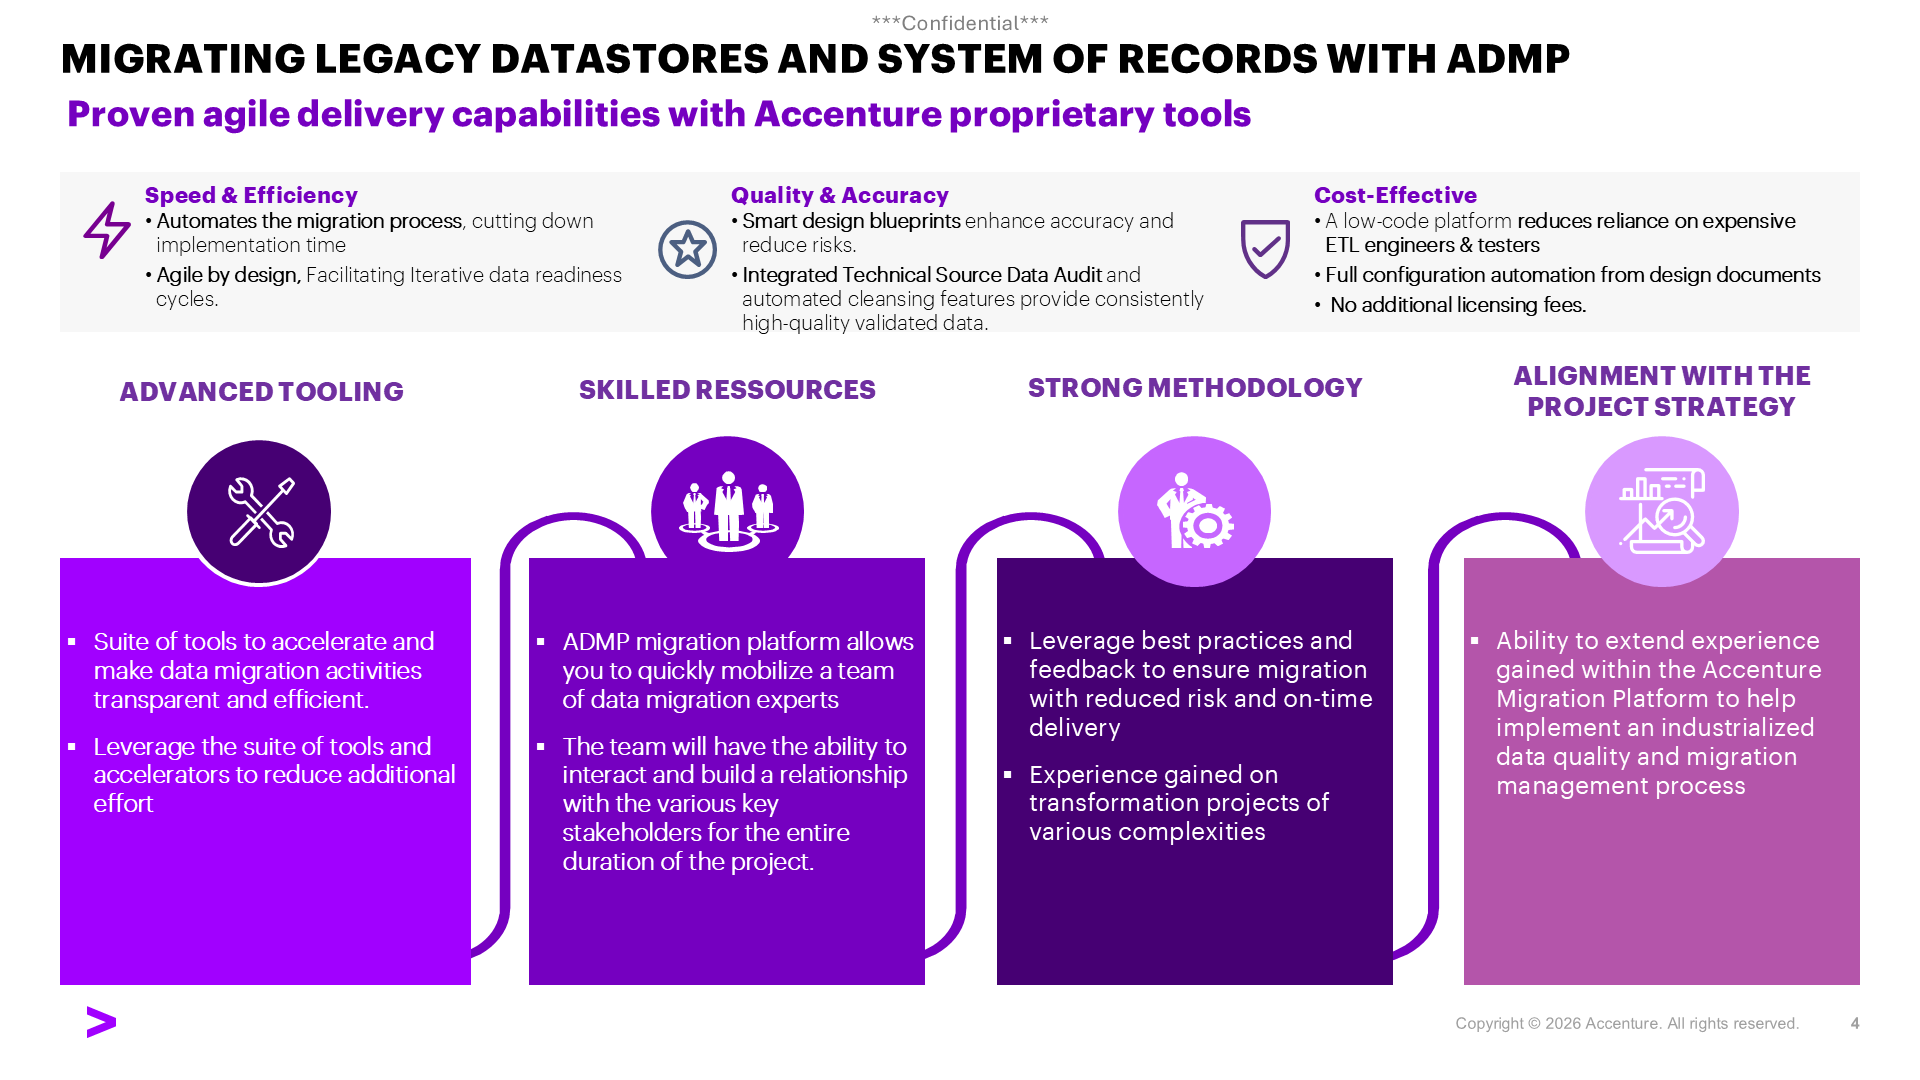
\includegraphics[width=0.85\textwidth]{img/admp_pillars.png}
    \caption{Les quatre piliers de valeur de la plateforme ADMP}
    \label{fig:admp-pillars}
\end{figure}

La valeur d'ADMP repose sur quatre piliers complémentaires qui structurent l'offre de service :

\begin{itemize}[leftmargin=*]
    \item \textbf{Advanced Tooling} : une suite d'outils et d'accélérateurs permettant de rendre les activités de migration transparentes et efficaces, et d'en réduire la charge additionnelle.
    \item \textbf{Skilled Resources} : la capacité à mobiliser rapidement une équipe d'experts en migration de données, capable d'interagir avec l'ensemble des parties prenantes tout au long du projet.
    \item \textbf{Strong Methodology} : un ensemble de meilleures pratiques éprouvées et validées, de la phase de découverte jusqu'au déploiement, garantissant une livraison dans les délais avec un risque réduit. \og~\textit{Experience gained on transformation projects of various complexities}~\fg{}.
    \item \textbf{Alignment with the Project Strategy} : la capacité à étendre l'expérience acquise sur la plateforme pour aider à mettre en \oe uvre un processus industrialisé de gestion de la qualité et de la migration des données.
\end{itemize}

% ---------------------------------------------------------------------
\subsubsection{Un service de migration sur mesure}
\label{subsubsec:admp-service}

\begin{figure}[H]
    \centering
    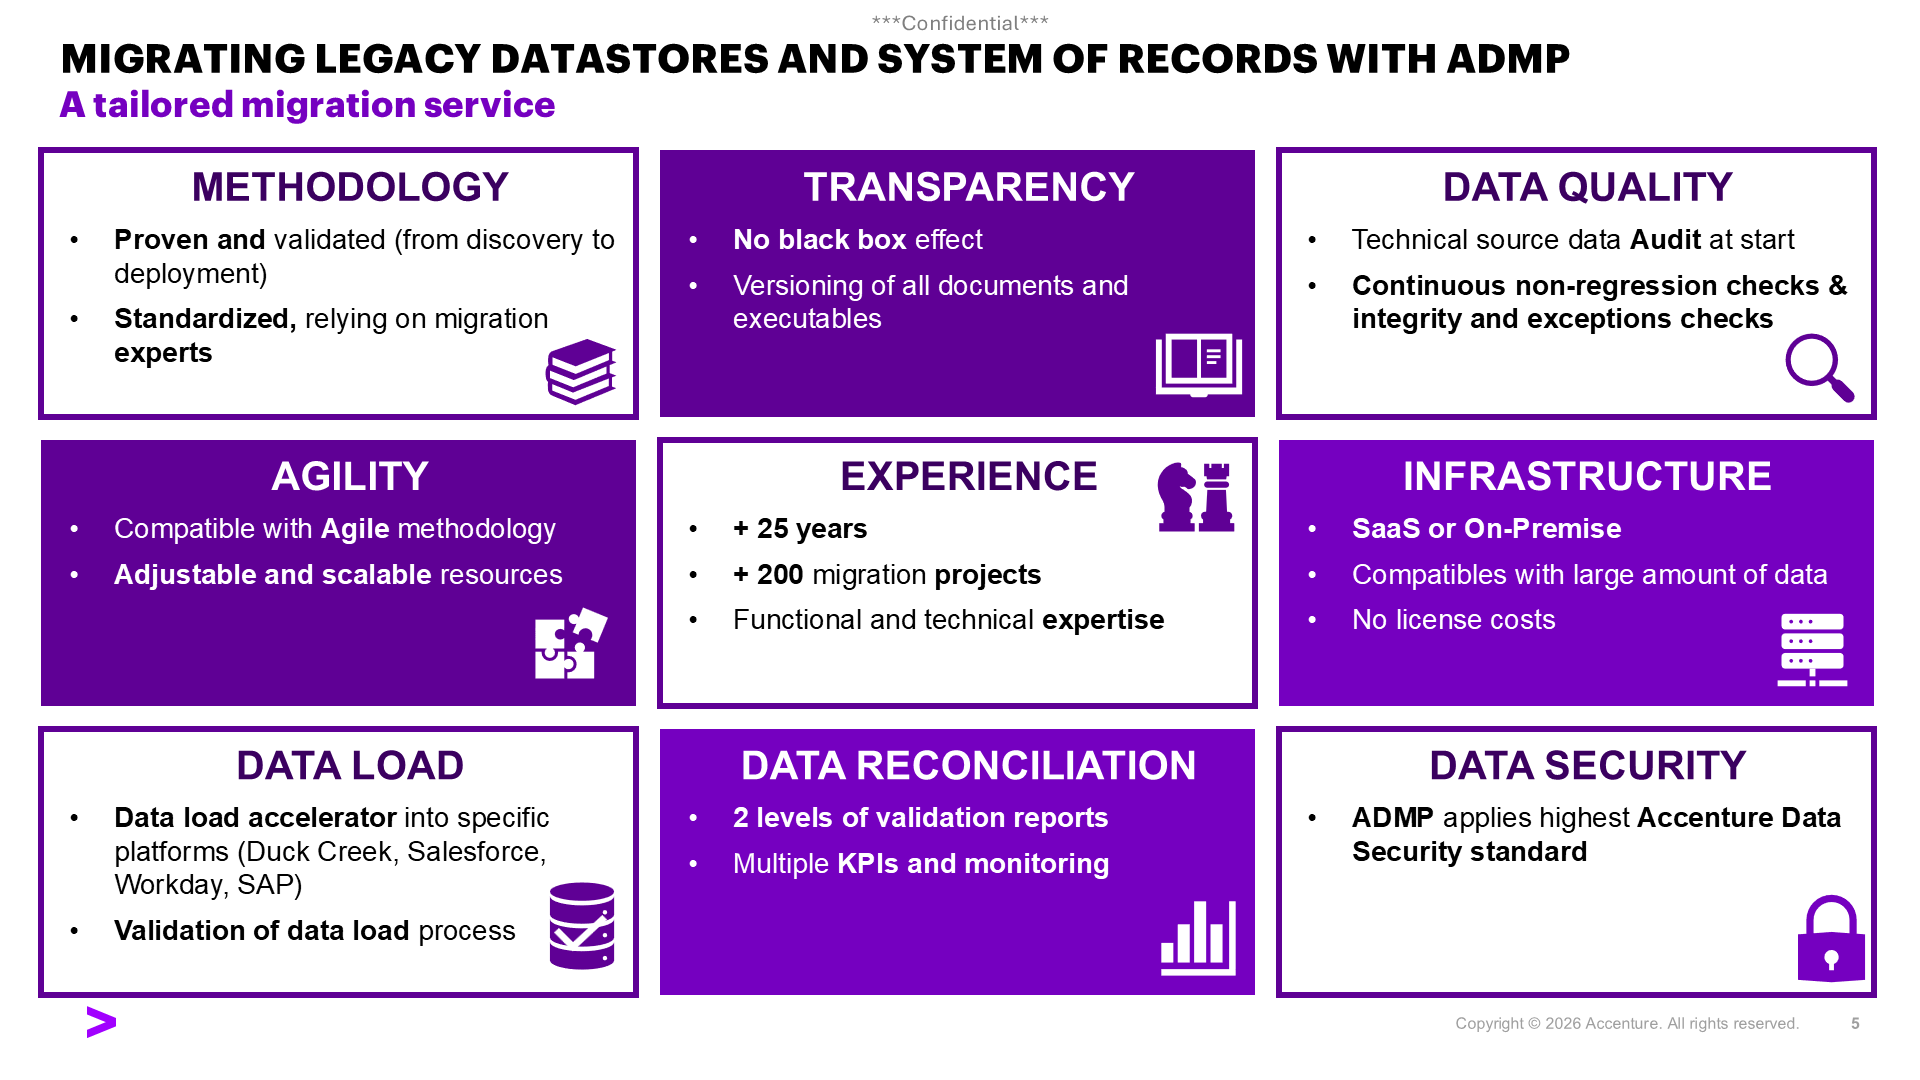
\includegraphics[width=0.85\textwidth]{img/admp_service_dimensions.png}
    \caption{Les neuf dimensions du service de migration sur mesure ADMP}
    \label{fig:admp-service}
\end{figure}

ADMP propose un service de migration global articulé autour de neuf dimensions clés :

\begin{itemize}[leftmargin=*]
    \item \textbf{Methodology} : méthodologie éprouvée et validée (de la découverte au déploiement), standardisée, s'appuyant sur des experts en migration.
    \item \textbf{Agility} : compatible avec les méthodes Agile, avec des ressources ajustables et scalables.
    \item \textbf{Data Load} : accélérateur de chargement vers des plateformes spécifiques (Duck Creek, Salesforce, Workday, SAP) avec validation du processus de chargement.
    \item \textbf{Transparency} : \og~\textit{No black box effect}~\fg{}, avec versioning de tous les documents et exécutables.
    \item \textbf{Experience} : +25 ans, +200 projets de migration, expertise fonctionnelle et technique.
    \item \textbf{Data Reconciliation} : 2 niveaux de rapports de validation, multiples KPIs et monitoring.
    \item \textbf{Data Quality} : audit technique des données source en amont, contrôles de non-régression continus, vérifications d'intégrité et gestion des exceptions.
    \item \textbf{Infrastructure} : SaaS ou On-Premise, compatible avec de grands volumes de données, sans coût de licence.
    \item \textbf{Data Security} : application des normes de sécurité des données les plus strictes d'Accenture.
\end{itemize}

% ---------------------------------------------------------------------
\subsubsection{Architecture end-to-end : le flux ETL ADMP}
\label{subsubsec:admp-etl}

\begin{figure}[H]
    \centering
    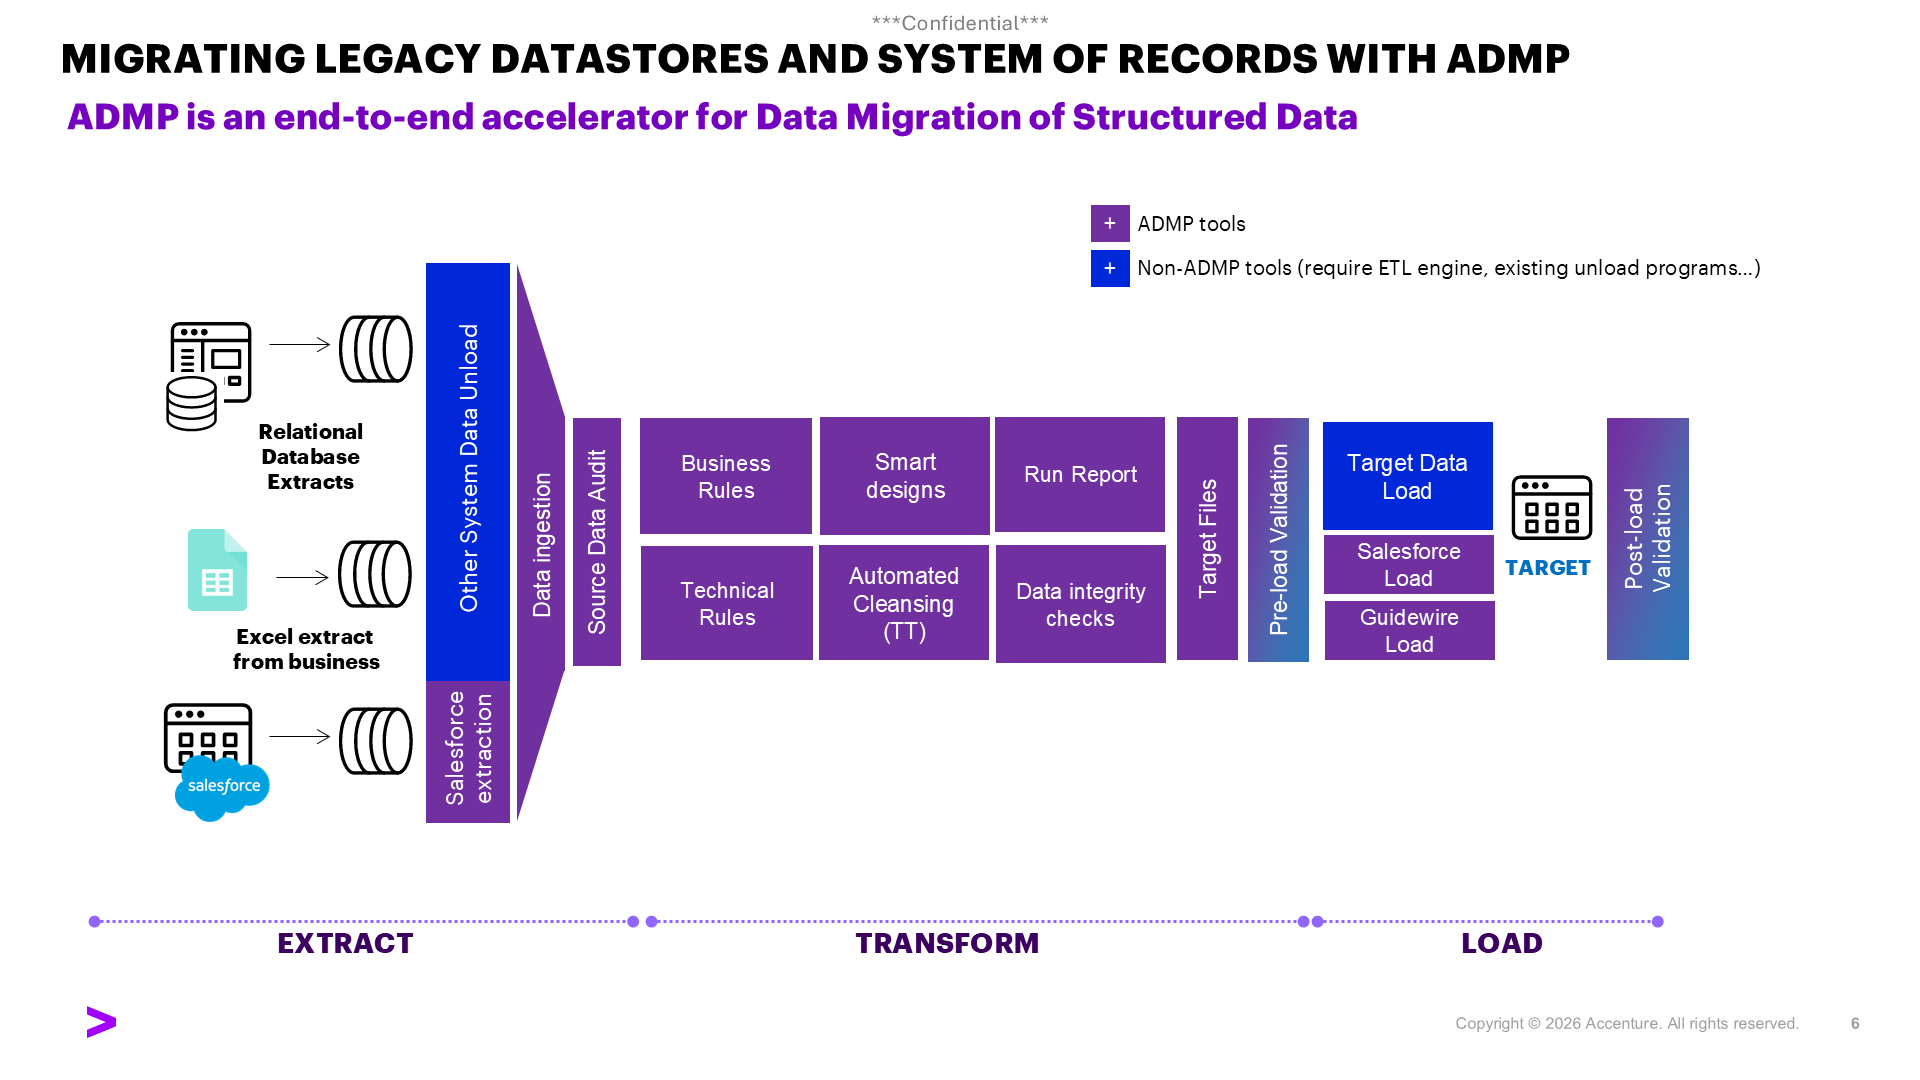
\includegraphics[width=\textwidth]{img/admp_etl_flow.png}
    \caption{Architecture end-to-end du flux ETL ADMP (Extract → Transform → Load)}
    \label{fig:admp-etl}
\end{figure}

Pour comprendre la valeur réelle d'ADMP, il convient de suivre le parcours d'une donnée depuis son système source jusqu'au système cible, en traversant chaque composant de la plateforme. Cette architecture, illustrée par la Figure~\ref{fig:admp-etl}, s'inscrit dans le modèle classique \textbf{Extract-Transform-Load (ETL)}, mais chaque phase est enrichie de composants propriétaires ADMP qui automatisent et sécurisent le processus. Il est important de noter que la plateforme distingue deux catégories de composants : les \textbf{outils ADMP} (développés et maîtrisés par Accenture) qui constituent le c\oe ur de la valeur ajoutée, et les \textbf{outils non-ADMP} (spécifiques aux systèmes source et cible du client) qui assurent les interfaces d'entrée et de sortie.

\paragraph{Phase 1 : Extract --- La collecte sécurisée des données sources.}

Le processus débute par l'extraction des données depuis les systèmes legacy du client. Ces données peuvent provenir de sources hétérogènes : bases de données relationnelles (Oracle, SQL Server, DB2, Mainframe), fichiers Excel fournis par les équipes métier, ou environnements Salesforce existants. À ce stade, les programmes d'\textit{unload} utilisés sont des outils \textbf{non-ADMP} : chaque système legacy dispose de son propre mécanisme d'export, que l'équipe adapte au contexte du projet.

Une fois extraits, les fichiers (généralement au format TXT ou CSV) sont pris en charge par le composant \textbf{Data Ingestion}, premier composant \textbf{ADMP} du pipeline. Celui-ci ingère les données dans la plateforme via un protocole de transfert sécurisé (SFTP, VPN), garantissant la confidentialité et l'intégrité des données dès leur entrée dans le périmètre Accenture.

\paragraph{Phase 2 : Transform --- Le c\oe ur de valeur d'ADMP.}

La phase de transformation est celle où ADMP déploie l'essentiel de son intelligence. Elle s'articule en deux couches fonctionnelles complémentaires.

La \textit{première couche} est dédiée à l'\textbf{audit et à la définition des règles}. Le composant \textbf{Source Data Audit} procède à un audit technique automatique et exhaustif de chaque table, enregistrement et champ source : il valide la complétude de l'extraction, détecte les anomalies de format et produit un état des lieux précis des données disponibles. C'est sur cette base que l'équipe de design commence son travail. Les \textbf{Business Rules} (règles métier fonctionnelles, correspondant aux documents RC --- \textit{Record Creation}) et les \textbf{Smart Designs} (l'ensemble des documents de spécification SDS, IDS, TDS, DS, DP, TT) constituent la \textit{source unique de vérité} du projet : le moteur ADMP lit ces documents et génère automatiquement les programmes de transformation, sans aucun développement ETL manuel. Chaque exécution produit un \textbf{Run Report}, rapport automatique de statistiques, d'erreurs et de volumétrie.

La \textit{deuxième couche} assure le \textbf{nettoyage et le contrôle qualité}. Les \textbf{Technical Rules} appliquent les transformations techniques (formats, longueurs, types de données). Le composant \textbf{Automated Cleansing (TT)} exploite les Tables de Transcodification pour normaliser automatiquement les valeurs source vers les valeurs cibles (mappings de codes, constantes, règles de substitution). Enfin, les \textbf{Data Integrity Checks} vérifient la cohérence référentielle entre tables, l'absence de doublons et la complétude des relations, avant que les données ne soient présentées au chargement.

\paragraph{Phase 3 : Load --- Le chargement encadré vers la cible.}

La phase de chargement est délibérément encadrée par deux niveaux de validation. La \textbf{Pre-load Validation} constitue une ultime vérification de conformité, d'intégrité et de volumétrie avant que les données ne quittent la plateforme ADMP vers le système cible. Elle permet de détecter en amont tout écart susceptible de provoquer une erreur lors du chargement.

Le chargement lui-même s'effectue via des composants \textbf{non-ADMP}, propres à chaque système cible : chargement vers des fichiers ou bases de données génériques (\textit{Target Data Load}), chargement spécifique vers Salesforce via Data Loader ou Bulk API, ou vers Guidewire via ses APIs d'import métier. Cette architecture intentionnellement ouverte permet à ADMP d'interfacer avec n'importe quelle plateforme cible du marché (Duck Creek, SAP, Vitech, Workday, etc.) sans dépendance technologique.

Le cycle se clôt par la \textbf{Post-load Validation}, composant ADMP qui effectue la réconciliation entre les volumes de données sources et cibles, contrôle la complétude du chargement et produit les rapports de migration finaux. C'est ce dernier rapport qui constitue la preuve de bonne exécution présentée au client.

\paragraph{Synthèse : quatre niveaux de validation intégrés.}

L'une des forces distinctives de l'architecture ADMP réside dans l'intégration systématique de quatre niveaux de validation tout au long du pipeline : l'\textbf{audit source} (avant le design), les \textbf{contrôles d'intégrité} (durant la transformation), la \textbf{validation pré-chargement} et la \textbf{validation post-chargement}. Cette approche élimine l'\textit{effet boîte noire} des solutions ETL traditionnelles et garantit une traçabilité complète, de la donnée source jusqu'à la donnée migrée dans le système cible.

% ---------------------------------------------------------------------
\subsubsection{Smart Designs vs ETL standard}
\label{subsubsec:admp-vs-etl}

\begin{figure}[H]
    \centering
    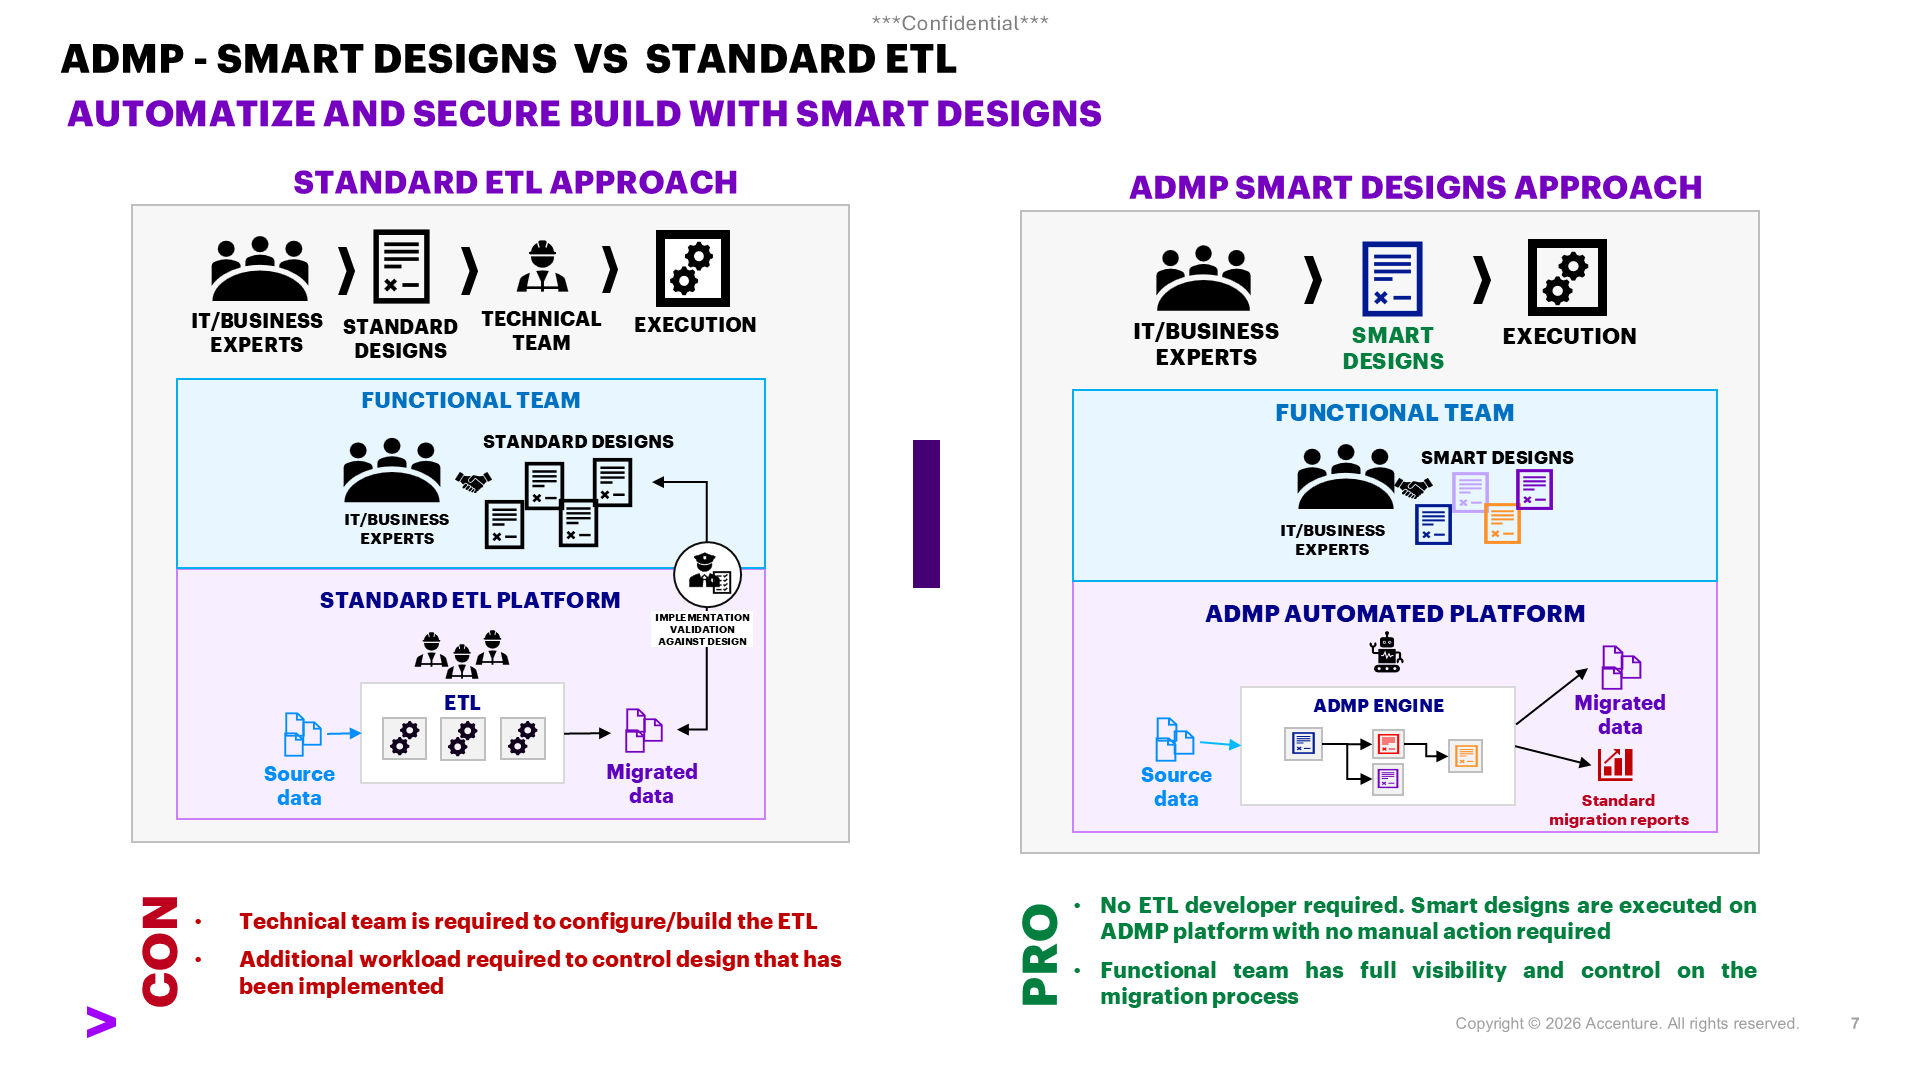
\includegraphics[width=0.85\textwidth]{img/admp_smartdesigns_vs_etl.png}
    \caption{Comparaison visuelle ADMP Smart Designs vs Standard ETL}
    \label{fig:admp-vs-etl}
\end{figure}

La comparaison entre l'approche ADMP Smart Designs et l'approche ETL traditionnelle met en évidence des avantages structurels significatifs, synthétisés dans le Tableau~\ref{tab:admp-vs-etl}.

\begin{table}[H]
\centering
\caption{Comparaison ADMP Smart Designs vs ETL standard}
\label{tab:admp-vs-etl}
\begin{tabularx}{\textwidth}{lXX}
\toprule
\textbf{Domaine} & \textbf{ETL Standard} & \textbf{ADMP Smart Designs} \\
\midrule
Build & Équipe technique requise (Talend, Informatica, BODS) & Aucun développeur ETL requis \\
\addlinespace
Rapports & Développés en supplément de l'ETL & Générés automatiquement depuis les Smart Designs \\
\addlinespace
Scalabilité & Contrainte par l'équipe technique et les outils & Gérée par design, templates hautement distribués \\
\addlinespace
Réutilisabilité & Compétences techniques avancées requises & Personnalisation facile (Word/Excel) \\
\addlinespace
Mises à jour des règles & Mise à jour simultanée des documents \textit{et} de l'ETL & Mise à jour du Smart Design uniquement \\
\addlinespace
Traçabilité & Impossible de valider design vs implémentation & Une seule source de vérité, traçabilité complète \\
\addlinespace
Licence & Coût de licence requis & Aucun coût de licence \\
\bottomrule
\end{tabularx}
\end{table}

% ---------------------------------------------------------------------
\subsubsection{La méthodologie ADMP : notre approche détaillée}
\label{subsubsec:admp-approche}

La méthodologie ADMP structure la migration en quatre phases, chacune impliquant des rôles précis côté client et côté Accenture.

\paragraph{Phase 1 --- Extraction des données.}

\begin{figure}[H]
    \centering
    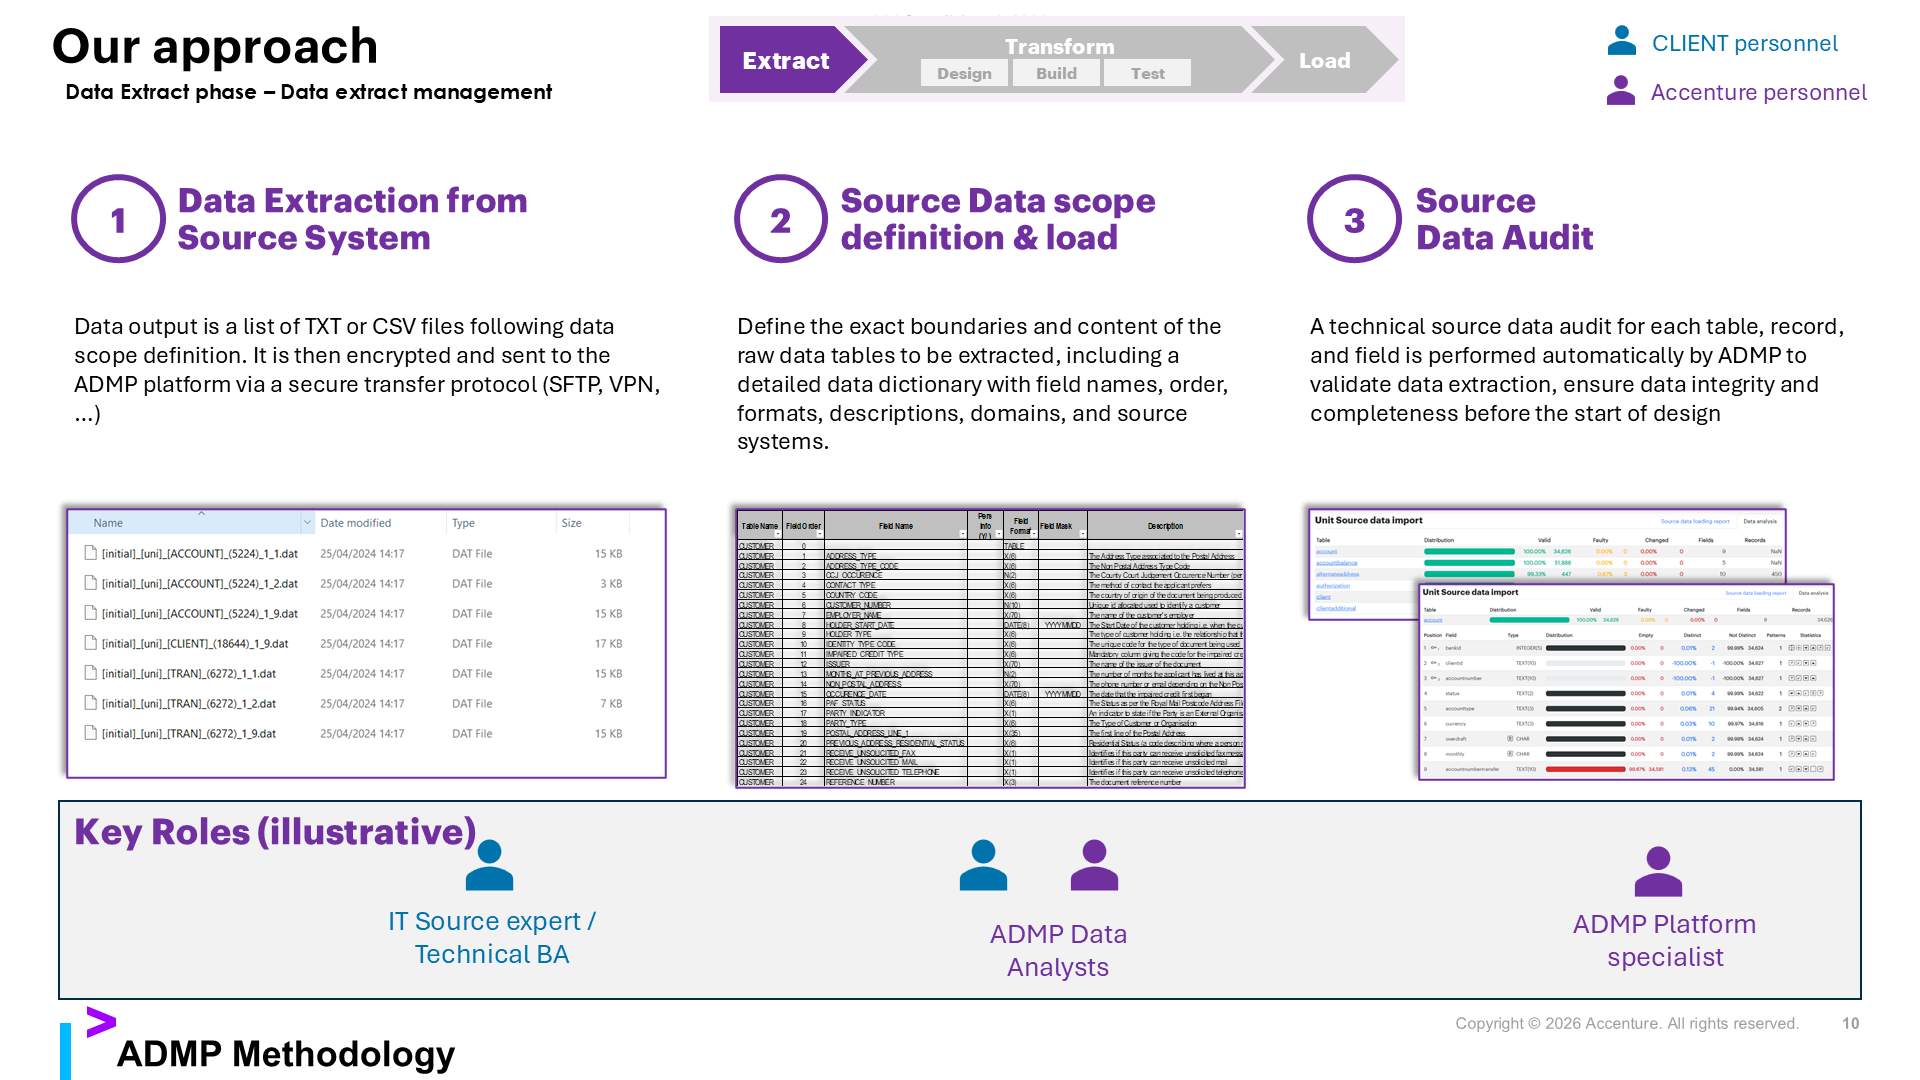
\includegraphics[width=\textwidth]{img/admp_approach_extract.png}
    \caption{Phase d'extraction -- Rôles et activités ADMP}
    \label{fig:admp-extract}
\end{figure}

Cette phase comprend trois étapes : (1) la \textbf{définition du périmètre et chargement} des données source, incluant un dictionnaire de données détaillé (noms de champs, formats, descriptions, domaines et systèmes source) ; (2) l'\textbf{extraction} des données depuis le système source vers des fichiers TXT ou CSV, chiffrés et transmis via SFTP/VPN ; (3) l'\textbf{audit technique automatique} des données source par table, enregistrement et champ.

\paragraph{Phase 2 --- Design (Analyse et Conception détaillée).}

\begin{figure}[H]
    \centering
    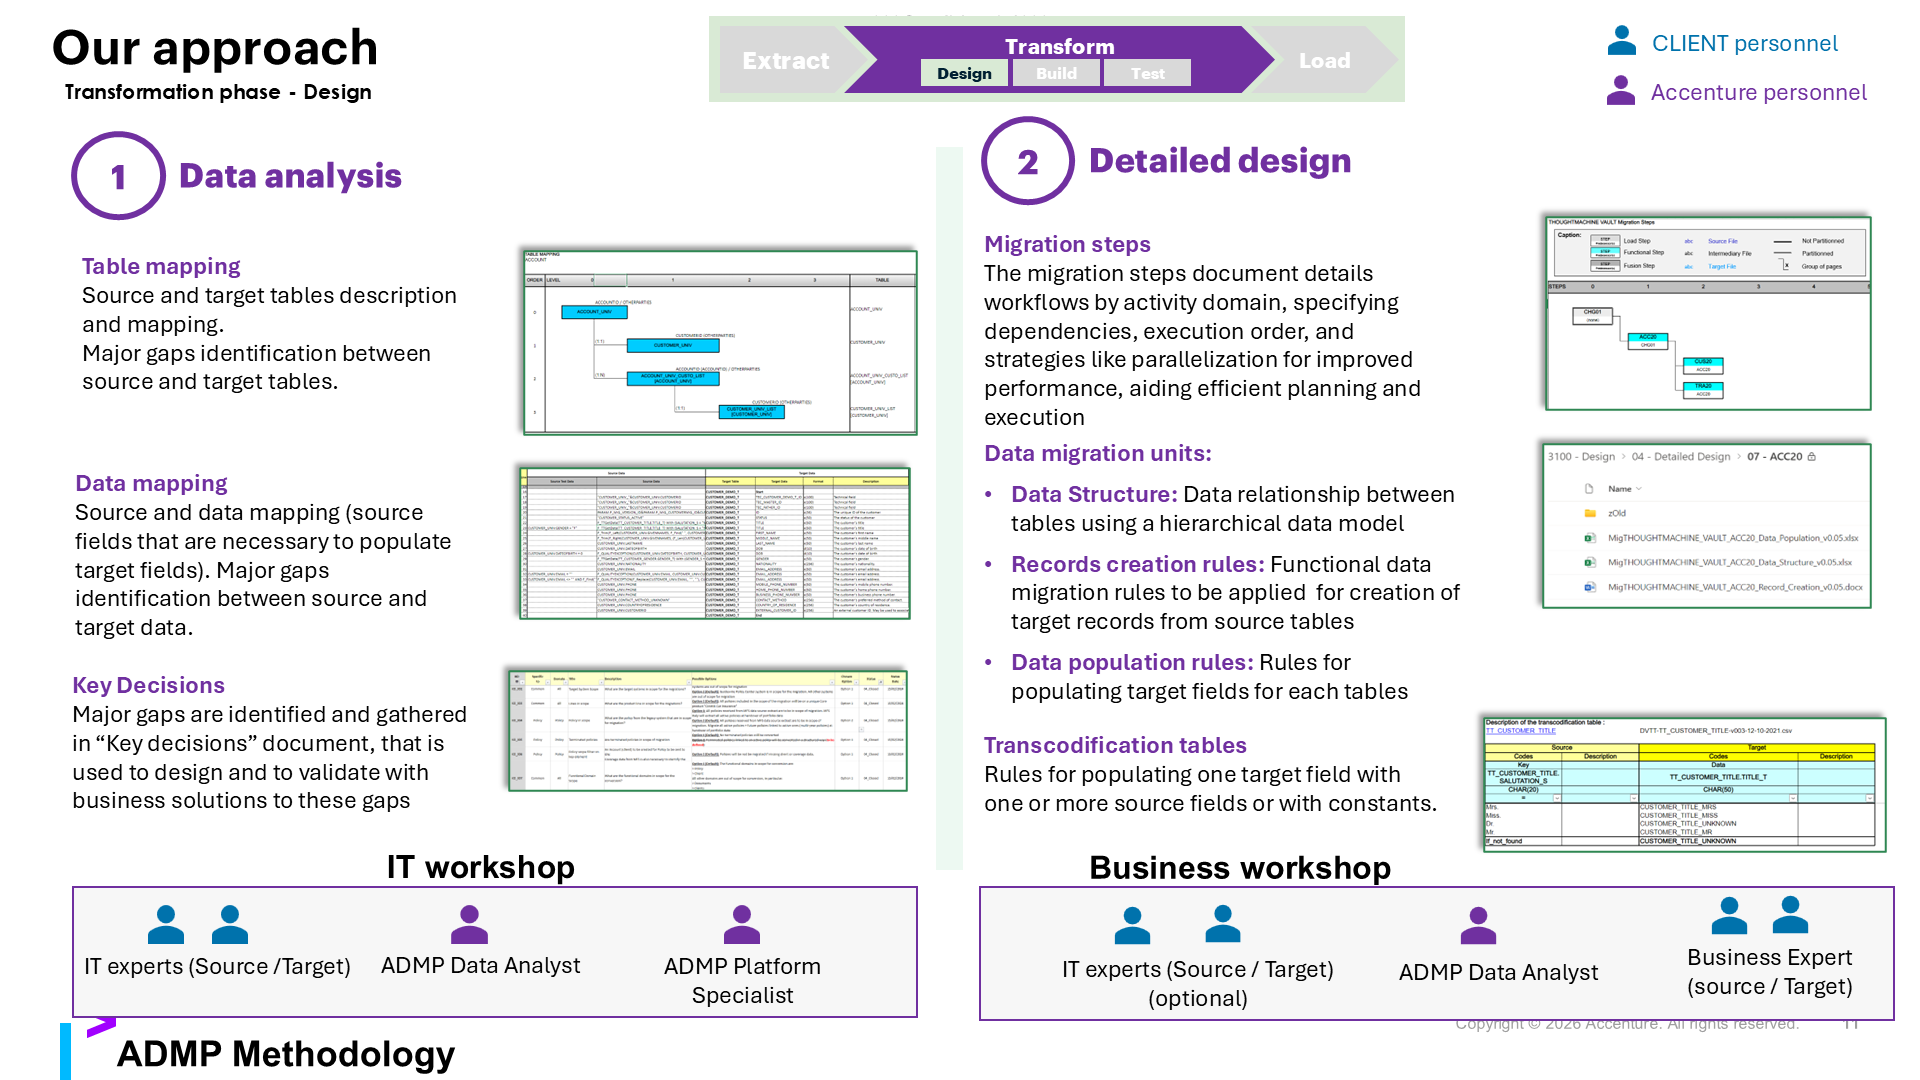
\includegraphics[width=\textwidth]{img/admp_approach_design.png}
    \caption{Phase de design -- Analyse et conception détaillée ADMP}
    \label{fig:admp-design}
\end{figure}

Organisée en deux volets : (1) l'\textbf{analyse de données} (Table Mapping, Data Mapping, Key Decisions pour les écarts majeurs), validée en workshops IT et Business ; (2) la \textbf{conception détaillée} comprenant les Migration Steps (workflows par domaine avec dépendances et stratégies de parallélisation), les Transcodification Tables, et les Data Migration Units (Data Structure, Record Creation, Data Population).

\paragraph{Phase 3 --- Build.}

\begin{figure}[H]
    \centering
    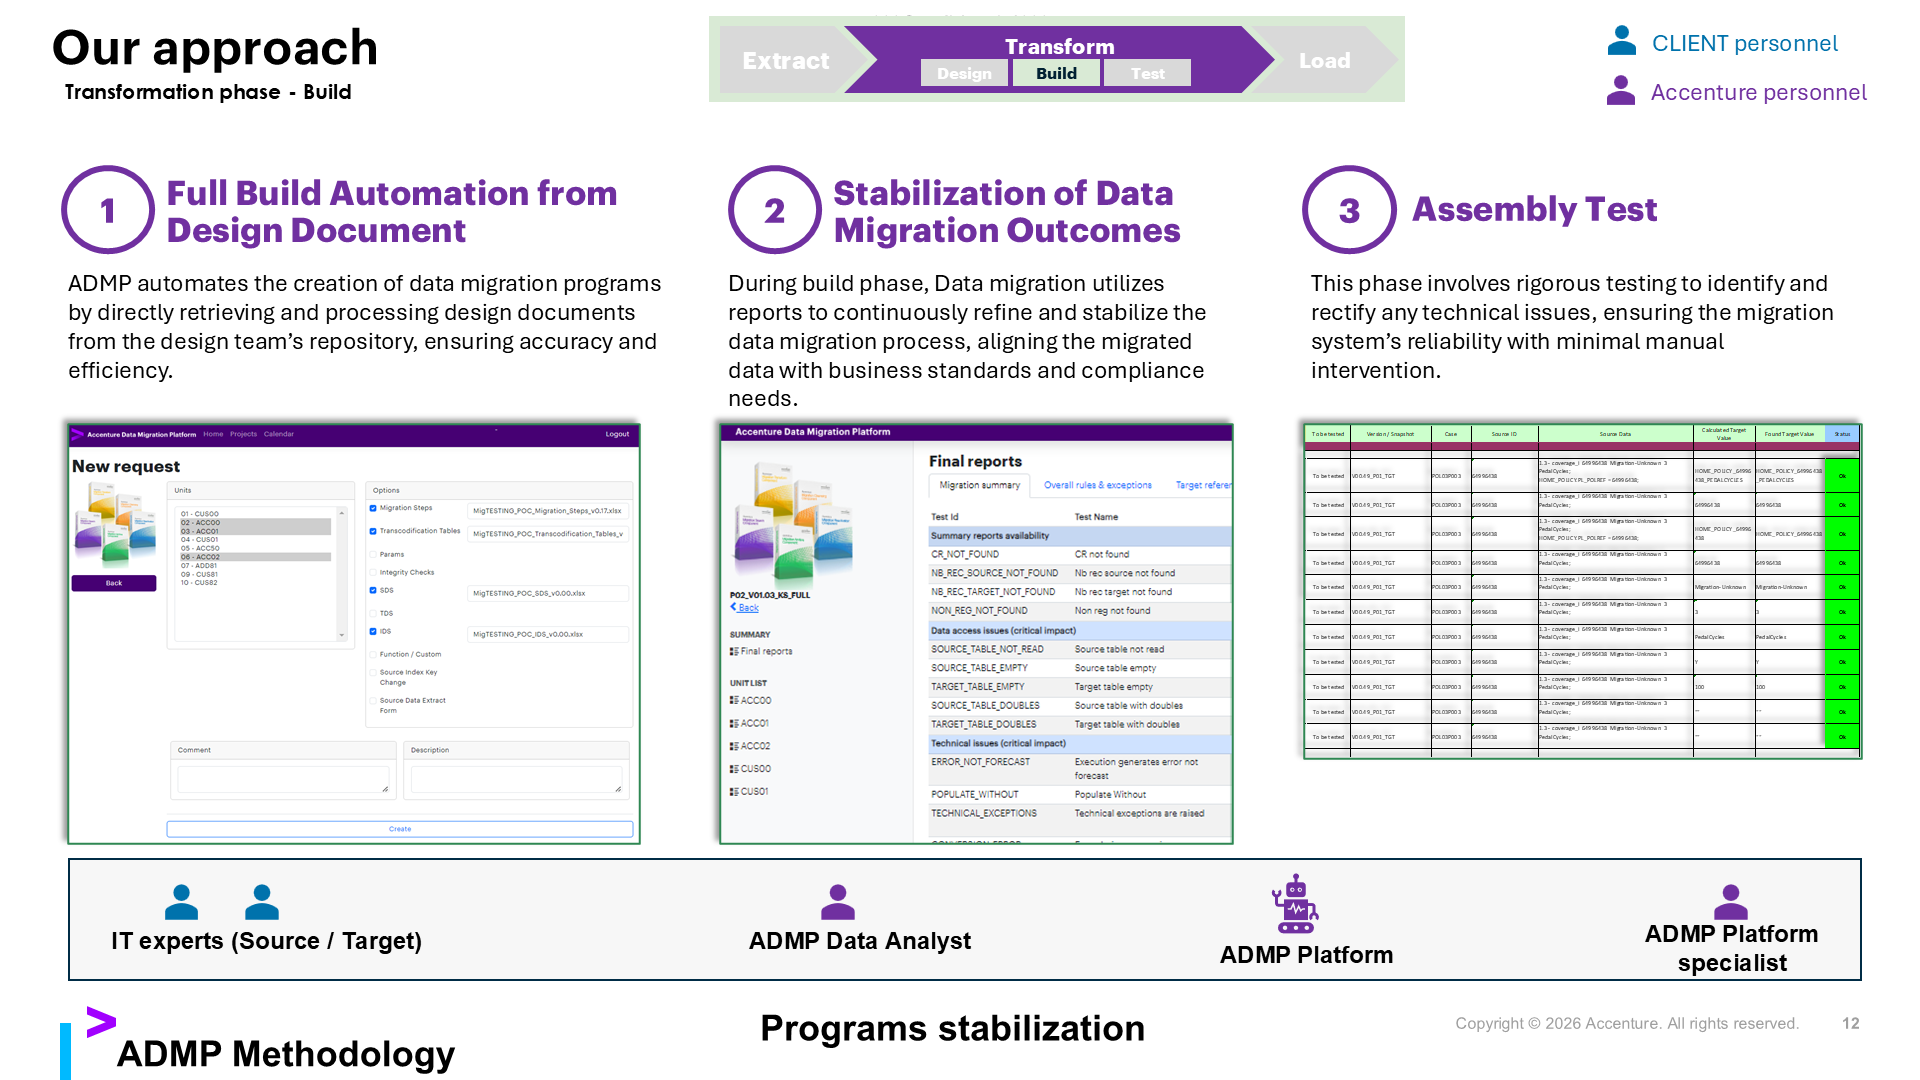
\includegraphics[width=\textwidth]{img/admp_approach_build.png}
    \caption{Phase de build -- Automatisation complète depuis les Smart Designs}
    \label{fig:admp-build}
\end{figure}

ADMP automatise intégralement la création des programmes de migration depuis les documents de design : (1) \textbf{Full Build Automation} -- le moteur récupère et traite directement les documents depuis le dépôt de l'équipe design ; (2) \textbf{Assembly Test} -- tests rigoureux pour identifier et corriger les problèmes techniques avec un minimum d'intervention manuelle ; (3) \textbf{Stabilisation} -- raffinement continu du processus à l'aide des rapports, pour aligner les données migrées avec les standards métier et de conformité.

\paragraph{Phase 4 --- Test et Déploiement.}

\begin{figure}[H]
    \centering
    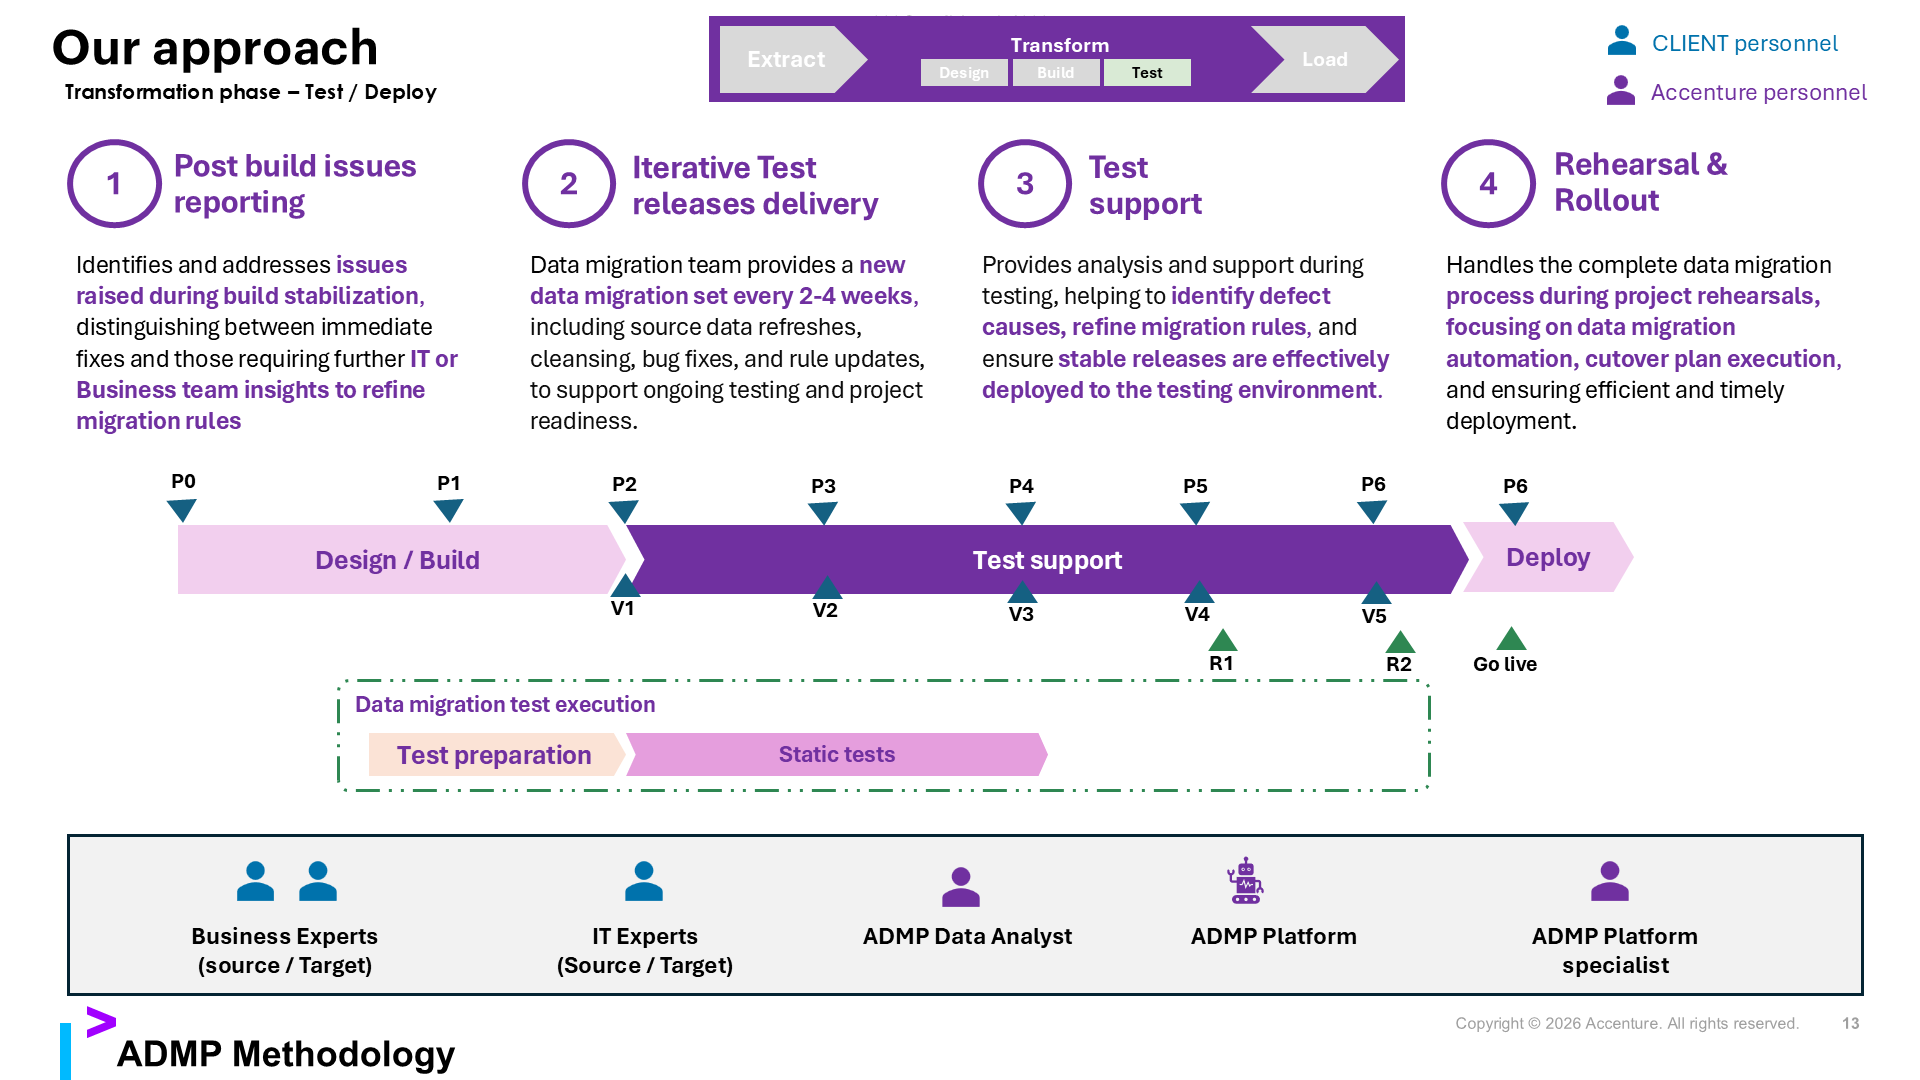
\includegraphics[width=\textwidth]{img/admp_approach_test_deploy.png}
    \caption{Phase de test et déploiement -- Cycle itératif ADMP}
    \label{fig:admp-test-deploy}
\end{figure}

La phase suit un cycle itératif organisé autour de : (1) \textbf{Post-build issues reporting} -- identification des anomalies, distinguant les correctifs immédiats des sujets nécessitant l'input des équipes IT ou Business ; (2) \textbf{Livraisons itératives de releases test} -- une nouvelle version toutes les 2 à 4 semaines (refresh des données source, corrections, mises à jour des règles) ; (3) \textbf{Test support} -- analyse et support lors des tests, identification des causes de défauts et affinement des règles ; (4) \textbf{Rehearsal \& Rollout} -- gestion complète du processus lors des répétitions (\textit{rehearsals}) et exécution du plan de bascule (\textit{cutover}).

% =====================================================================
\subsection{Intelligence artificielle et intégration de données}
\label{subsec:ia-integration}

% ---------------------------------------------------------------------
\subsubsection{LLM et génération de code (GPT, Mistral, fine-tuning, LoRA)}
\label{subsubsec:llm}

Les \textbf{Large Language Models (LLM)} ont révolutionné le domaine de la génération automatique de code et de la compréhension du langage naturel. Des modèles comme GPT-4, Llama 3, Claude et Mistral sont capables de générer du code SQL, Python ou PySpark à partir de spécifications en langage naturel, ouvrant des perspectives considérables pour l'automatisation des processus de migration.

La technique de \textbf{LoRA (Low-Rank Adaptation)}, introduite par Hu et al. (2021), a transformé l'approche du fine-tuning en permettant d'adapter des modèles de plusieurs milliards de paramètres avec une fraction des ressources habituellement nécessaires. LoRA gèle les poids du modèle pré-entraîné et injecte des matrices de rang faible entraînables dans chaque couche, réduisant les paramètres entraînables de \textbf{99\%+} tout en atteignant \textbf{95-98\% de la performance} d'un fine-tuning complet.

Concrètement, le fine-tuning d'un modèle Llama 3.1 70B passe de \textbf{8 GPU A100 pendant 48 heures ($\sim$15 000 \$)} en fine-tuning complet à \textbf{1 GPU A100 pendant 4 heures ($\sim$500 \$)} avec LoRA. Cette démocratisation rend le fine-tuning accessible pour des cas d'usage spécifiques à un domaine, comme la génération de règles de transformation de données.

La variante \textbf{QLoRA} combine LoRA avec une quantification 4-bit, permettant le fine-tuning sur du matériel grand public, une avancée particulièrement pertinente pour les équipes ne disposant pas d'infrastructure GPU dédiée.

\begin{figure}[H]
    \centering
    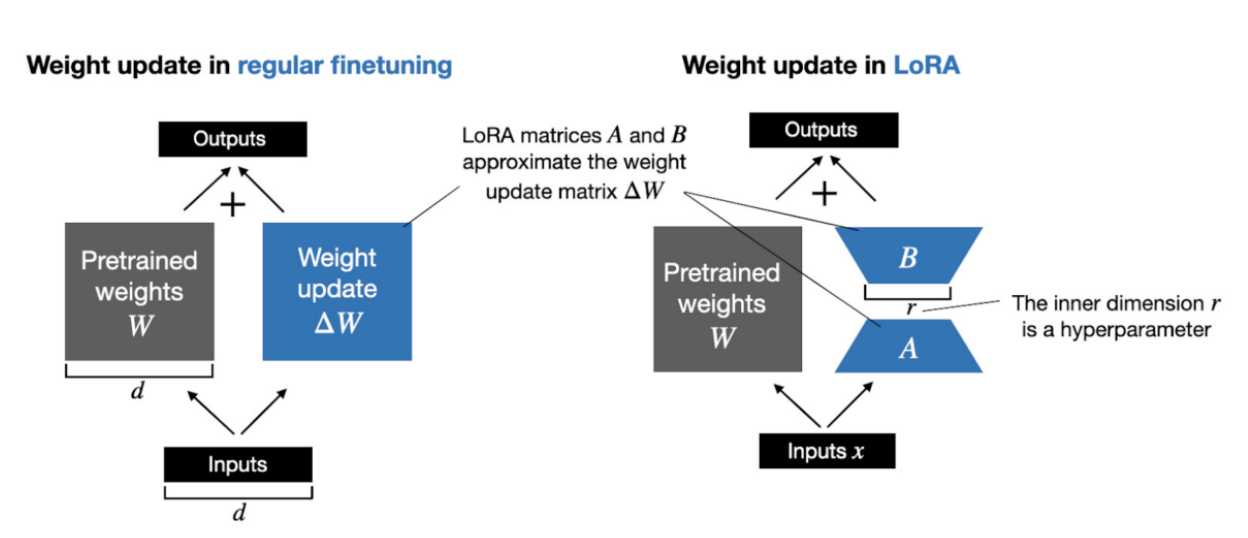
\includegraphics[width=0.8\textwidth]{img/LoRa.png}
    \caption{Principe du fine-tuning avec LoRA (Low-Rank Adaptation)}
    \label{fig:lora}
\end{figure}

% ---------------------------------------------------------------------
\subsubsection{RAG (Retrieval-Augmented Generation)}
\label{subsubsec:rag}

Le \textbf{RAG (Retrieval-Augmented Generation)}, introduit par Lewis et al. (2020), est une architecture qui enrichit les LLM en les couplant avec des sources de connaissances externes au moment de l'inférence. Plutôt que de s'appuyer uniquement sur les connaissances intériorisées lors de l'entraînement, le RAG récupère dynamiquement des passages pertinents depuis une base documentaire et les injecte dans le contexte du modèle pour générer des réponses factuellement ancrées.

L'architecture RAG se décompose en deux composants principaux :

\begin{itemize}[leftmargin=*]
    \item \textbf{Le composant de récupération} : les requêtes sont encodées en vecteurs denses, puis comparées aux vecteurs de documents pré-encodés dans une base vectorielle (FAISS, pgvector, Pinecone). Les passages les plus pertinents sont extraits.
    
    \item \textbf{Le composant de génération} : les documents récupérés sont combinés avec la requête pour produire une réponse contextuelle et précise via le LLM.
\end{itemize}

Microsoft propose une architecture RAG de référence dans Azure Architecture Center, intégrant Azure AI Search, Semantic Kernel et des modèles de langage pour construire des applications d'entreprise robustes.

Dans le contexte de la migration de données, le RAG permet d'exploiter la documentation existante (SDS, TDS, RC, DP) comme base de connaissances pour assister les spécificateurs dans la rédaction de règles, la résolution de questions fonctionnelles, et la validation des designs.

\begin{figure}[H]
    \centering
    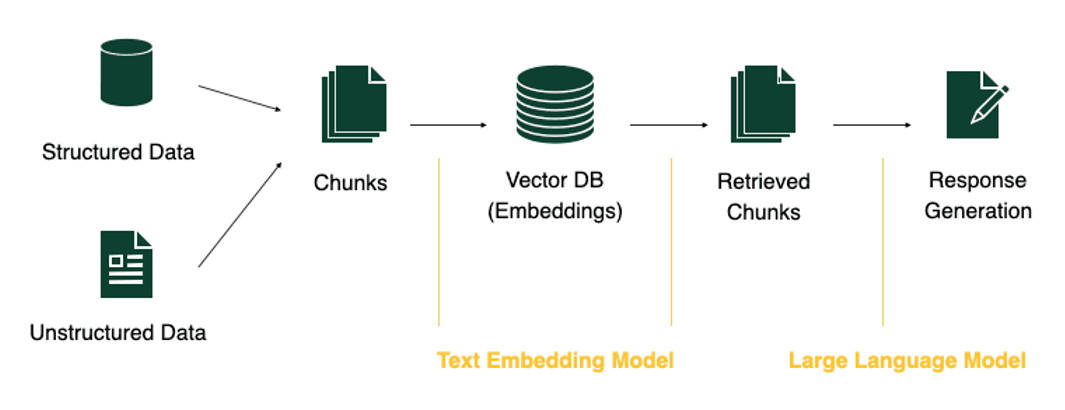
\includegraphics[width=0.9\textwidth]{img/RAG.png}
    \caption{Architecture Retrieval-Augmented Generation (RAG)}
    \label{fig:rag-architecture}
\end{figure}

% ---------------------------------------------------------------------
\subsubsection{Agents IA et automatisation de workflows}
\label{subsubsec:agents-ia}

Les \textbf{agents IA} représentent une évolution majeure par rapport à l'automatisation traditionnelle. Contrairement aux systèmes RPA (\textit{Robotic Process Automation}) qui suivent des scripts prédéfinis, les agents IA combinent perception, raisonnement et action pour accomplir des objectifs de manière autonome.

Leurs caractéristiques distinctives incluent :

\begin{itemize}[leftmargin=*]
    \item \textbf{Autonomie} : fonctionnement indépendant sans supervision constante.
    \item \textbf{Conscience contextuelle} : compréhension des scénarios métier nuancés.
    \item \textbf{Raisonnement multi-étapes} : décomposition de tâches complexes en sous-tâches exécutables.
    \item \textbf{Auto-correction} : identification et rectification des erreurs en cours d'exécution.
    \item \textbf{Intégration d'outils} : connexion transparente avec APIs, bases de données et systèmes d'entreprise.
\end{itemize}

Le marché mondial des agents IA est estimé à \textbf{5,1 milliards USD en 2024}, avec une projection à \textbf{47,1 milliards USD d'ici 2030} (CAGR de 44,8\%). Toutefois, selon Gartner (2025), moins de \textbf{5\% des applications d'entreprise intègrent de véritables agents IA} à ce stade, la majorité n'utilisant que des assistants basiques.

% ---------------------------------------------------------------------
\subsubsection{Applications de l'IA dans la migration de données}
\label{subsubsec:ia-migration}

L'application de l'IA au domaine spécifique de la migration de données est un champ émergent mais prometteur, avec cinq cas d'usage à fort impact identifiés par Blackburn (2025) :

\begin{itemize}[leftmargin=*]
    \item \textbf{Mapping automatique de schémas} : les modèles ML analysent la structure, le contenu et les métadonnées des sources pour suggérer des correspondances source-cible, réduisant le temps de mapping de \textbf{30-60\%}.
    
    \item \textbf{Évaluation et nettoyage de la qualité} : les LLM détectent les anomalies que les règles statiques ne capturent pas, et peuvent suggérer des actions de nettoyage automatiques.
    
    \item \textbf{Génération de données synthétiques de test} : les modèles génératifs produisent des jeux de test réalistes préservant les propriétés statistiques sans exposer de données réelles.
    
    \item \textbf{Planification intelligente de la migration} : le reinforcement learning optimise l'ordonnancement des lots de migration en fonction des dépendances et des contraintes de fenêtre.
    
    \item \textbf{Monitoring et détection d'anomalies en production} : des pipelines de détection identifient les écarts en temps réel et accélèrent le triage des erreurs.
\end{itemize}

La plateforme \textbf{MAiGRATE} de Compliance Group illustre cette tendance : elle combine IA, ML et LLM pour automatiser l'ingestion, la transformation, le mapping de champs, la déduplication, la détection d'anomalies et la validation, avec un apprentissage continu améliorant la précision à chaque cycle de migration.

% =====================================================================
\subsection{Limites de l'existant et opportunités}
\label{subsec:limites-opportunites}

% ---------------------------------------------------------------------
\subsubsection{Limites des outils de design actuels}
\label{subsubsec:limites-design}

Les Design Tools actuels d'ADMP reposent sur des \textbf{plugins VBA intégrés à Word et Excel}. Si cette approche a l'avantage d'utiliser des outils familiers aux équipes fonctionnelles, elle présente des limitations de plus en plus critiques :

\begin{itemize}[leftmargin=*]
    \item \textbf{Technologie vieillissante} : VBA est un langage de macro datant des années 1990, dont le support et l'évolutivité sont limités.
    \item \textbf{Pas de collaboration en temps réel} : contrairement aux outils web modernes, les documents Word/Excel ne permettent pas l'édition simultanée avec traçabilité fine.
    \item \textbf{Intégration IA impossible} : l'architecture VBA ne permet pas d'intégrer nativement des appels à des API d'IA (OpenAI, Bedrock) pour assister la rédaction.
    \item \textbf{Maintenance complexe} : les macros VBA sont fragiles, sensibles aux versions d'Office, et difficiles à déboguer.
\end{itemize}

% ---------------------------------------------------------------------
\subsubsection{Rédaction manuelle des spécifications}
\label{subsubsec:redaction-manuelle}

La rédaction des spécifications de migration (RC, DP, DS, TT) reste un processus \textbf{largement manuel et chronophage}. Chaque document nécessite une compréhension approfondie du modèle source, du modèle cible, et des règles métier spécifiques. Comme le souligne la présentation d'évolution ADMP, l'un des objectifs stratégiques de la modernisation est de \og~\textit{Optimize and accelerate the time needed to write specifications}~\fg{} et de \og~\textit{Create a true wizard for specifiers and reduce the overall burden}~\fg{}.

Le rapport PFE de Abbad el andaloussi, Larbi estime que l'automatisation de la génération des livrables de migration permettrait une \textbf{réduction de 50 à 60\% du temps} nécessaire à leur production, tout en minimisant les risques d'erreurs humaines.

% ---------------------------------------------------------------------
\subsubsection{Absence d'IA dans le processus de migration}
\label{subsubsec:absence-ia}

Malgré les avancées considérables de l'IA dans d'autres domaines de l'IT, le processus de migration ADMP reste \textbf{dépourvu d'intelligence artificielle}. Aucun module IA n'assiste actuellement les spécificateurs dans la rédaction des règles, la détection des incohérences, ou la validation automatique des designs. Cette absence représente une opportunité majeure d'amélioration.

% ---------------------------------------------------------------------
\subsubsection{Dépendance à l'expertise humaine}
\label{subsubsec:dependance-expertise}

La qualité de la migration repose fortement sur l'expertise individuelle des Data Analysts. L'\textbf{onboarding} de nouveaux membres nécessite une formation intensive (la CIDS dure \textbf{2 semaines (80 heures)}) et l'acquisition de la maturité opérationnelle prend plusieurs mois supplémentaires. Cette dépendance crée un risque de perte de connaissances (\textit{knowledge drain}) lors des rotations d'équipe et limite la scalabilité des opérations.

% =====================================================================
\subsection{Synthèse et positionnement de la contribution}
\label{subsec:synthese-positionnement}

% ---------------------------------------------------------------------
\subsubsection{Tableau de synthèse des gaps identifiés}
\label{subsubsec:gaps}

Le Tableau~\ref{tab:gaps-synthesis} synthétise les principaux gaps identifiés et les opportunités associées.

\begin{table}[H]
\centering
\caption{Synthèse des gaps identifiés et opportunités}
\label{tab:gaps-synthesis}
\begin{tabularx}{\textwidth}{XXX}
\toprule
\textbf{Gap identifié} & \textbf{Impact} & \textbf{Opportunité} \\
\midrule
Outils de design VBA obsolètes & Pas de collaboration, pas d'IA & → ADMP Studio (outil web moderne) \\
\addlinespace
Rédaction manuelle des spécifications & Chronophage, risque d'erreur & → ADMP AI Engine (génération assistée) \\
\addlinespace
Absence d'IA dans le processus & Aucune assistance intelligente & → Intégration LLM + RAG \\
\addlinespace
Dépendance à l'expertise humaine & Onboarding long, scalabilité limitée & → Assistant IA pour spécificateurs \\
\addlinespace
Pas de génération automatique de code & Build manuel des programmes & → Bundle Databricks (notre contribution) \\
\bottomrule
\end{tabularx}
\end{table}

% ---------------------------------------------------------------------
\subsubsection{Positionnement du PFE}
\label{subsubsec:positionnement-pfe}

L'analyse de l'état de l'art révèle que la plateforme ADMP, malgré sa maturité et ses avantages concurrentiels significatifs, se trouve à un tournant stratégique. Les outils existants ont prouvé leur efficacité pendant plus de 25 ans, mais l'absence d'intelligence artificielle dans le processus constitue désormais un frein à l'innovation et à la compétitivité.

Le programme d'évolution d'ADMP, articulé autour de l'\textbf{ADMP AI Engine}, de l'\textbf{ADMP Studio} et de l'amélioration des outils de design, vise à combler ces gaps.

Notre contribution, le \textbf{développement du module de génération du bundle Databricks}, s'inscrit précisément dans cet axe d'industrialisation. Ce module vise à automatiser la création des artefacts de migration en s'appuyant sur des technologies de traitement distribué (Apache Spark / Databricks) et d'intelligence artificielle générative, transformant ainsi les Smart Designs en programmes exécutables sur des infrastructures cloud modernes.

Ce positionnement se situe à l'intersection de trois tendances identifiées dans l'état de l'art : l'\textbf{automatisation du cycle Design-Build} (section~\ref{subsec:admp-actuel}), l'\textbf{application de l'IA à la migration} (section~\ref{subsec:ia-integration}), et le besoin de \textbf{modernisation des outils} (section~\ref{subsec:limites-opportunites}). Le chapitre suivant présentera le cadre méthodologique et organisationnel dans lequel ce travail a été réalisé.
% =====================================================================
% CHAPITRE 4 — CADRE MÉTHODOLOGIQUE ET GESTION DE PROJET
% =====================================================================
\chapter{Cadre Méthodologique et Gestion de Projet}
\label{chap:methodologie}

Le chapitre précédent a identifié les fondements théoriques, les solutions existantes et les opportunités d'amélioration qui positionnent notre contribution. Avant de détailler la conception de notre solution (chapitre~5), il est essentiel de présenter le cadre méthodologique et organisationnel dans lequel s'inscrit ce travail. Ce chapitre décrit comment l'équipe ADMP s'organise au quotidien pour mener à bien ses projets de migration : la méthodologie Agile adoptée, le cycle de vie des tickets, les processus de validation des données, et les pratiques collaboratives qui assurent la cohésion et l'efficacité de l'équipe.

% =====================================================================
\section{Méthodologie Agile adoptée}
\label{sec:methodologie-agile}

% ---------------------------------------------------------------------
\subsection{Principes Scrum appliqués au projet}
\label{subsec:scrum}

Le cadre de travail adopté au sein de l'équipe ADMP s'inspire du framework \textbf{Scrum}, la méthodologie Agile la plus répandue au monde, utilisée par près de \textbf{87\,\%} des équipes Agile selon le \textit{State of Agile Report} \cite{digitalai2024}. Scrum repose sur trois piliers fondamentaux --- transparence, inspection et adaptation --- et s'articule autour de la règle \og~3-5-3~\fg{}, synthétisée dans le Tableau~\ref{tab:scrum-335}.

\begin{table}[H]
\centering
\caption{Le framework Scrum : règle 3-5-3}
\label{tab:scrum-335}
\begin{tabularx}{\textwidth}{lXX}
\toprule
\textbf{Composant} & \textbf{Éléments} & \textbf{Fonction} \\
\midrule
3 Rôles & Product Owner, Scrum Master, Développeurs & Définir les responsabilités et permettre l'auto-organisation \\
\addlinespace
5 Événements & Sprint, Sprint Planning, Daily Scrum, Sprint Review, Sprint Retrospective & Créer la régularité et permettre l'inspection-adaptation \\
\addlinespace
3 Artefacts & Product Backlog, Sprint Backlog, Increment & Maximiser la transparence et mesurer la progression \\
\bottomrule
\end{tabularx}
\end{table}

Dans le contexte spécifique de la migration de données, ces principes sont adaptés aux réalités du projet. Le \textbf{Product Owner} est représenté par le chef de projet migration, qui priorise les lots fonctionnels à migrer en fonction des besoins métier et des dépendances techniques. Le \textbf{Scrum Master} est incarné par le Team Lead ADMP, qui facilite les cérémonies, lève les blocages et veille au respect de la méthodologie. Les \textbf{Développeurs} correspondent aux Data Analysts ADMP, qui rédigent les spécifications (RC, DP, DS), analysent les données et valident les résultats de migration.

Les cinq valeurs Scrum --- engagement, courage, focus, ouverture et respect --- guident les interactions quotidiennes au sein de l'équipe, particulièrement dans les échanges avec le client lors des phases de validation et de prise de décision.

% ---------------------------------------------------------------------
\subsection{Organisation des sprints de migration}
\label{subsec:sprints}

L'approche ADMP structure le processus de migration en \textbf{sprints itératifs} d'une durée de 2 à 4 semaines, chacun livrant un nouveau jeu de données migré intégrant les corrections, les rafraîchissements de données source et les mises à jour des règles. Cette cadence régulière constitue le rythme fondamental du projet.

Chaque sprint de migration suit un enchaînement rigoureux de quatre phases :

\begin{itemize}[leftmargin=*]
    \item \textbf{Phase 1 --- Design / Build (Static Tests)} : les Data Analysts rédigent ou mettent à jour les spécifications (RC, DP, DS, TT), versionnées via IDMF Explorer. Le Core Engine génère automatiquement les programmes de migration. Des tests statiques valident la cohérence des règles avant toute exécution.
    \item \textbf{Phase 2 --- Test Support} : l'équipe analyse les défauts identifiés, identifie leurs causes racines et affine les règles de migration pour garantir la stabilité des versions livrées à l'environnement de test.
    \item \textbf{Phase 3 --- Stabilisation et livraison itérative} : des versions successives (V1, V2, V3, V4, V5\ldots) sont produites, chacune intégrant les corrections issues des cycles de test précédents, convergeant progressivement vers la qualité attendue.
    \item \textbf{Phase 4 --- Rehearsal \& Rollout} : l'équipe gère le processus complet de migration durant les répétitions générales (\textit{rehearsals}), en se concentrant sur l'automatisation de la migration, l'exécution du plan de bascule (\textit{cutover}) et le déploiement dans les délais impartis.
\end{itemize}

Le cycle complet d'un projet type suit la progression illustrée en Figure~\ref{fig:sprint-cycle}.

\begin{figure}[H]
\centering
\begin{tikzpicture}[
  ms/.style={circle, fill=accenturedark, text=white, font=\bfseries\scriptsize,
             minimum size=7mm, inner sep=0pt},
  rh/.style={circle, fill=accenturepurple, text=white, font=\bfseries\scriptsize,
             minimum size=7mm, inner sep=0pt},
  gl/.style={diamond, fill=accenturepurple, text=white, font=\bfseries\tiny,
             minimum size=10mm, inner sep=0pt},
  >=Latex, thick, color=accenturedark
]
  % --- Milestone nodes (absolute coordinates, 1.5 cm center-to-center) ---
  \node[ms] (p0) at (0,    0) {P0};
  \node[ms] (p1) at (1.5,  0) {P1};
  \node[ms] (p2) at (3.0,  0) {P2};
  \node[ms] (p3) at (4.5,  0) {P3};
  \node[ms] (p4) at (6.0,  0) {P4};
  \node[ms] (p5) at (7.5,  0) {P5};
  \node[ms] (p6) at (9.0,  0) {P6};
  \node[rh] (r1) at (10.5, 0) {R1};
  \node[rh] (r2) at (12.0, 0) {R2};
  \node[gl] (gl) at (13.5, 0) {};
  \node[below=2pt of gl, font=\scriptsize\bfseries, text=accenturepurple]
       {Go Live};

  % --- Arrows ---
  \foreach \s/\t in {p0/p1, p1/p2, p2/p3, p3/p4, p4/p5, p5/p6,
                     p6/r1, r1/r2}{
    \draw[->] (\s) -- (\t);
  }
  \draw[->, color=accenturepurple] (r2) -- (gl);

  % --- Phase brace : Design/Build/Test ---
  \draw[decorate,
        decoration={brace, mirror, amplitude=6pt},
        color=accenturedark, thick]
    ([yshift=-5mm]p0.south) -- ([yshift=-5mm]p6.south)
    node[midway, below=9pt, font=\small, align=center, text=accenturedark]
         {Design / Build / Test\\[-1pt]{\scriptsize(Versions V1--V5)}};

  % --- Phase brace : Rehearsals ---
  \draw[decorate,
        decoration={brace, mirror, amplitude=6pt},
        color=accenturepurple, thick]
    ([yshift=-5mm]r1.south) -- ([yshift=-5mm]r2.south)
    node[midway, below=9pt, font=\small, align=center, text=accenturepurple]
         {Rehearsals\\[-1pt]{\scriptsize(Répétitions)}};
\end{tikzpicture}
\caption{Cycle de progression d'un projet de migration ADMP}
\label{fig:sprint-cycle}
\end{figure}

Cette organisation permet de découvrir et de résoudre les problèmes de manière incrémentale, plutôt que de les accumuler jusqu'à un \og~Big Bang~\fg{} final risqué. L'approche Agile appliquée à la migration de données réduit considérablement les risques grâce à la validation précoce et continue, par opposition à l'approche traditionnelle où les tests ne sont conduits qu'après l'exécution complète \cite{datavail2025}.

% ---------------------------------------------------------------------
\subsection{Outils de pilotage}
\label{subsec:outils-pilotage}

L'outil central de pilotage du projet est \textbf{Azure DevOps}, une plateforme Microsoft conçue pour faciliter la collaboration entre les équipes de développement et d'exploitation dans l'esprit DevOps \cite{microsoft2025devops}. Le composant principal utilisé est \textbf{Azure Boards}, qui assure la gestion agile à travers les fonctionnalités suivantes :

\begin{itemize}[leftmargin=*]
    \item \textbf{Backlogs} : priorisation et planification du travail à venir au niveau des Epics, Features et User Stories.
    \item \textbf{Boards (Kanban)} : visualisation du flux de travail avec des colonnes représentant les états des tickets (\textit{New, Active, Resolved, Closed}).
    \item \textbf{Sprints} : planification des itérations avec distribution des tâches entre les membres de l'équipe.
    \item \textbf{Burndown Charts} : graphiques de suivi montrant le travail restant vs.\ la ligne idéale de progression, permettant de détecter rapidement les écarts et d'ajuster l'effort.
    \item \textbf{Dashboards} : tableaux de bord personnalisables agrégant les métriques clés du projet (vélocité, tendances de défauts, couverture de test).
    \item \textbf{Queries} : requêtes personnalisées pour filtrer et grouper les tickets selon différents critères (sévérité, assignation, état, sprint).
\end{itemize}

Azure Boards supporte les processus Agile, Scrum et CMMI, avec des types de \textit{work items} prédéfinis (Epic, Feature, User Story, Task, Bug) et des transitions d'état configurables \cite{microsoft2025boards}.

% =====================================================================
\section{Gestion des tickets et cycle de vie des défauts}
\label{sec:gestion-tickets}

% ---------------------------------------------------------------------
\subsection{Typologie des tickets}
\label{subsec:typologie-tickets}

Dans le contexte d'un projet de migration ADMP, les tickets Azure DevOps se déclinent en plusieurs types organisés hiérarchiquement, comme le résume le Tableau~\ref{tab:ticket-types}.

\begin{table}[H]
\centering
\caption{Hiérarchie des types de tickets Azure DevOps en contexte ADMP}
\label{tab:ticket-types}
\begin{tabularx}{\textwidth}{llX}
\toprule
\textbf{Type} & \textbf{Description} & \textbf{Exemple en migration} \\
\midrule
Epic    & Initiative stratégique de haut niveau & \og~Migration du domaine Opérations~\fg{} \\
\addlinespace
Feature & Fonctionnalité regroupant plusieurs User Stories & \og~Migration des Work Orders~\fg{} \\
\addlinespace
User Story & Besoin métier décrit du point de vue utilisateur & \og~Migrer les compétences des ressources de service~\fg{} \\
\addlinespace
Task    & Tâche technique unitaire & \og~Rédiger le RC du lot SKL01~\fg{} \\
\addlinespace
Bug / Defect & Anomalie identifiée lors des tests & \og~Team Leader name vide pour certains contrats~\fg{} \\
\bottomrule
\end{tabularx}
\end{table}

Cette hiérarchie (Epic $\rightarrow$ Feature $\rightarrow$ User Story $\rightarrow$ Task) permet une traçabilité complète depuis les objectifs stratégiques jusqu'aux tâches individuelles, et assure que chaque action est reliée à un besoin métier identifié.

% ---------------------------------------------------------------------
\subsection{Workflow d'un ticket de défaut}
\label{subsec:workflow-ticket}

Le cycle de vie d'un ticket de défaut dans le contexte ADMP suit un processus structuré en cinq étapes, illustré par la Figure~\ref{fig:ticket-workflow}.

\begin{figure}[H]
\centering
\begin{tikzpicture}[
  state/.style={rectangle, rounded corners=5pt,
                fill=accenturedark, text=white,
                font=\bfseries\small, minimum width=2.4cm,
                minimum height=1.1cm, align=center},
  role/.style={font=\scriptsize, text=accenturedark,
               align=center, text width=2.4cm},
  >=Latex, thick, color=accenturedark,
  node distance=0.7cm
]
  % --- State boxes ---
  \node[state]                          (new)  {CRÉATION\\\tiny(New)};
  \node[state, right=0.7cm of new]      (act)  {ANALYSE\\\tiny(Active)};
  \node[state, right=0.7cm of act]      (res)  {RÉSOLUTION\\\tiny(Resolved)};
  \node[state, right=0.7cm of res]      (val)  {VALIDATION\\\tiny(Test)};
  \node[state, right=0.7cm of val,
        fill=accenturepurple]           (clo)  {CLÔTURE\\\tiny(Closed)};

  % --- Arrows ---
  \draw[->] (new) -- (act);
  \draw[->] (act) -- (res);
  \draw[->] (res) -- (val);
  \draw[->] (val) -- (clo);

  % --- Role labels below ---
  \node[role, below=0.6cm of new]
       {Tester / Client détecte l'anomalie};
  \node[role, below=0.6cm of act]
       {Data Analyst identifie la root cause};
  \node[role, below=0.6cm of res]
       {Data Analyst corrige les Smart Designs};
  \node[role, below=0.6cm of val]
       {Tester vérifie le fix (nouveau snapshot)};
  \node[role, below=0.6cm of clo]
       {QA / PM valide la clôture};
\end{tikzpicture}
\caption{Cycle de vie d'un ticket de défaut ADMP (5 états)}
\label{fig:ticket-workflow}
\end{figure}

\paragraph{Étape 1 --- Création.}
Le testeur ou le client identifie une anomalie dans les données migrées et crée un ticket avec une description détaillée (étapes de reproduction, résultat attendu vs.\ résultat obtenu, captures d'écran). Le ticket est assigné au Data Analyst responsable du domaine fonctionnel concerné.

\paragraph{Étape 2 --- Analyse (Root Cause).}
Le Data Analyst identifie la cause racine du défaut en examinant les spécifications de migration. Cette analyse s'appuie sur une méthodologie rigoureuse : consultation du SDS/IDS/TDS pour vérifier les noms exacts des champs, du DS pour la structure hiérarchique et les clés de jointure, du RC pour les règles de création d'enregistrements, et du DP pour les règles de peuplement des champs.

\paragraph{Étape 3 --- Résolution.}
Le Data Analyst implémente la correction dans les Smart Designs. Celle-ci peut prendre la forme d'une modification de règle RC/DP, d'un ajout de transcodification, d'un \textit{data patch} SQL, ou d'une mise à jour de la structure DS. La résolution est documentée dans le champ \og~\textit{Resolution Action}~\fg{} du ticket.

\paragraph{Étape 4 --- Validation.}
Après génération d'un nouveau snapshot de données, le testeur vérifie que le défaut est corrigé et qu'aucune régression n'a été introduite dans les données précédemment validées.

\paragraph{Étape 5 --- Clôture.}
Une fois la validation réussie, le ticket est marqué \og~Closed~\fg{} avec les commentaires de validation confirmant la correction effective.

% ---------------------------------------------------------------------
\subsection{Priorisation et classification}
\label{subsec:priorisation}

Les défauts sont classifiés selon deux axes complémentaires qui déterminent l'ordre de traitement, comme le précise le Tableau~\ref{tab:severite-priorite}.

\begin{table}[H]
\centering
\caption{Axes de classification des défauts}
\label{tab:severite-priorite}
\begin{tabularx}{\textwidth}{llX}
\toprule
\textbf{Axe} & \textbf{Niveaux} & \textbf{Description} \\
\midrule
Sévérité & Critical / High / Medium / Low &
Impact technique du défaut sur le système : données corrompues, perte d'enregistrements, incohérence référentielle\ldots \\
\addlinespace
Priorité & P1 (Urgente) / P2 (Haute) / P3 (Moyenne) / P4 (Basse) &
Urgence de résolution du point de vue métier : périmètre fonctionnel impacté, criticité pour le Go Live\ldots \\
\bottomrule
\end{tabularx}
\end{table}

La distinction entre \textbf{sévérité} et \textbf{priorité} est essentielle : un défaut peut être techniquement critique (données corrompues) mais de priorité moyenne s'il ne concerne qu'un périmètre limité, ou inversement. Des réunions de triage hebdomadaires permettent à l'équipe de réévaluer les priorités en fonction de l'avancement du projet et des retours du client.

% ---------------------------------------------------------------------
\subsection{Exemple de cycle complet d'un défaut}
\label{subsec:exemple-defaut}

Pour illustrer concrètement le processus, considérons un défaut typique rencontré en projet de migration. Le Tableau~\ref{tab:exemple-defaut} détaille le cycle complet du ticket suivant : \og~Le champ \texttt{Team Leader} est vide pour certains Work Orders alors qu'il devrait être renseigné.~\fg{}

\begin{table}[H]
\centering
\caption{Exemple de cycle complet d'un ticket de défaut}
\label{tab:exemple-defaut}
\begin{tabularx}{\textwidth}{llX}
\toprule
\textbf{Étape} & \textbf{Action} & \textbf{Détail} \\
\midrule
1. Création & Ticket créé par le testeur &
Pour un contrat donné, 6 Work Orders ont le champ \texttt{CER\_TEAMLEADER\_\_C} vide \\
\addlinespace
2. Analyse & Identification de la root cause &
Le RC du lot WRK01 filtre les Work Orders par flag (Y/N), mais ne couvre pas le cas où le flag est Y et le champ source correspondant est NULL \\
\addlinespace
3. Résolution & Modification du RC/DP &
Ajout d'une condition dans le RC pour gérer le cas \texttt{Flag = Y AND Source\_TL IS NULL}, avec fallback vers le Service Resource principal \\
\addlinespace
4. Validation & Nouveau snapshot P20.3 &
Requête SQL de vérification : \textbf{0 cas KO} dans le nouveau snapshot (vs.\ 132 dans P20.1 et 32 dans P20.2) \\
\addlinespace
5. Clôture & Ticket fermé &
Commentaire : \og~Fix validé --- régression zéro --- confirmé par comparaison P20.1 $\rightarrow$ P20.2 $\rightarrow$ P20.3~\fg{} \\
\bottomrule
\end{tabularx}
\end{table}

Ce cycle illustre l'approche systématique de l'équipe : chaque défaut est tracé de bout en bout, avec une documentation complète de l'analyse, de la correction et de la validation.

% =====================================================================
\section{Processus de validation des données}
\label{sec:validation}

% ---------------------------------------------------------------------
\subsection{Snapshots et cycles de test}
\label{subsec:snapshots}

Le processus de validation repose sur un mécanisme de \textbf{snapshots} --- des extractions complètes des données à un instant donné --- qui servent de base aux cycles de test successifs. Chaque snapshot est identifié par un code de version (P20.1, P20.2, P20.3\ldots) et représente l'état des données après application des dernières corrections.

La progression entre les snapshots suit une logique de convergence vers la qualité cible, illustrée par la Figure~\ref{fig:snapshot-convergence}. À chaque nouveau snapshot, l'équipe vérifie que les défauts précédemment identifiés sont corrigés (test de non-régression) et qu'aucun nouveau défaut n'a été introduit par les corrections.

\begin{figure}[H]
\centering
\begin{tikzpicture}[
  >=Latex, thick,
  ms/.style={circle, fill=accenturedark, text=white,
             font=\bfseries\tiny, minimum size=6mm, inner sep=0pt},
  rh/.style={circle, fill=accenturepurple, text=white,
             font=\bfseries\tiny, minimum size=6mm, inner sep=0pt},
  gl/.style={diamond, fill=accenturepurple, text=white,
             font=\bfseries\tiny, minimum size=8mm, inner sep=0pt},
  lbl/.style={font=\scriptsize, align=center, text width=2.2cm}
]
  % --- Timeline ---
  \node[ms] (p0) at (0,   0) {P0};
  \node[ms] (p1) at (2.0, 0) {P1};
  \node[ms] (p2) at (4.0, 0) {P2};
  \node[ms] (pn) at (6.5, 0) {Pn};
  \node[rh] (r1) at (9.0, 0) {R1};
  \node[rh] (r2) at (11.0,0) {R2};
  \node[gl] (gl) at (13.0,0) {};
  \node[below=2pt of gl, font=\scriptsize\bfseries, text=accenturepurple] {Go Live};

  % --- Arrows (dashed between p2 and pn) ---
  \draw[->] (p0) -- (p1);
  \draw[->] (p1) -- (p2);
  \draw[->, dashed, color=accenturedark!60] (p2) -- (pn)
      node[midway, above, font=\tiny, text=accenturedark!80] {\ldots};
  \draw[->] (pn) -- (r1);
  \draw[->, color=accenturepurple] (r1) -- (r2);
  \draw[->, color=accenturepurple] (r2) -- (gl);

  % --- Defect annotations ---
  \node[lbl, above=8pt of p0] {\scriptsize Beaucoup de KO};
  \node[lbl, above=8pt of p1] {\scriptsize Corrections majeures};
  \node[lbl, above=8pt of p2] {\scriptsize Affinements};
  \node[lbl, above=8pt of pn] {\scriptsize Quasi-stable};

  % --- Brace: nombre de défauts décroissant ---
  \draw[decorate,
        decoration={brace, amplitude=6pt},
        color=accenturedark!70]
    ([yshift=30pt]p0.north) -- ([yshift=30pt]gl.north)
    node[midway, above=8pt, font=\small, text=accenturedark!80, align=center]
    {Nombre de défauts décroissant};
\end{tikzpicture}
\caption{Convergence progressive des snapshots vers la qualité cible}
\label{fig:snapshot-convergence}
\end{figure}

% ---------------------------------------------------------------------
\subsection{Stratégie de test}
\label{subsec:strategie-test}

La stratégie de test adoptée dans les projets de migration ADMP couvre trois niveaux complémentaires \cite{datagaps2025,quinnox2025} :

\begin{enumerate}[leftmargin=*, label=\textbf{\arabic*.}]
    \item \textbf{Tests unitaires (par lot de migration)} --- Chaque lot de migration (ex.\ : SKL01, WRK01, RES01) est testé individuellement pour vérifier que les règles de création (RC) et de peuplement (DP) produisent les résultats attendus. Les Data Analysts rédigent des requêtes SQL ciblées pour contrôler les cas nominaux et les cas limites.

    \item \textbf{Tests d'intégration (inter-lots)} --- Les relations entre les lots de migration sont vérifiées pour garantir l'intégrité référentielle. Par exemple, un Work Order doit pointer vers un Service Contract existant, et un ServiceResourceSkill doit référencer un ServiceResource et un Skill valides. Ces tests détectent les incohérences de clés étrangères et les enregistrements orphelins.

    \item \textbf{Tests de réconciliation} --- La réconciliation compare les volumes de données entre la source et la cible à plusieurs niveaux de granularité : nombre total d'enregistrements par table, sommes de contrôle sur les champs numériques, et vérification d'échantillons aléatoires. L'objectif est de garantir qu'aucune donnée n'a été perdue, dupliquée ou altérée durant le processus \cite{datafold2025}.
\end{enumerate}

% ---------------------------------------------------------------------
\subsection{Rapports de validation et KPIs}
\label{subsec:rapports-validation}

La plateforme ADMP génère automatiquement plusieurs types de rapports de validation, consultables via l'\textbf{ADMP Portal}, synthétisés dans le Tableau~\ref{tab:rapports-validation}.

\begin{table}[H]
\centering
\caption{Rapports de validation automatiques de la plateforme ADMP}
\label{tab:rapports-validation}
\begin{tabularx}{\textwidth}{llX}
\toprule
\textbf{Rapport} & \textbf{Phase} & \textbf{Contenu} \\
\midrule
Load Report        & Post-extraction    & Confirmation du chargement réussi des fichiers source dans la base SQL Server \\
\addlinespace
Data Audit         & Post-extraction    & KPIs sur les données sources : complétude, distribution des valeurs, détection d'anomalies \\
\addlinespace
DS Audit           & Post-design        & Validation de la cohérence des Data Structures (relations hiérarchiques) \\
\addlinespace
Integrity Check    & Post-transformation & Vérification de l'intégrité référentielle entre les tables cibles \\
\addlinespace
Run Report         & Post-transformation & Statistiques d'exécution : enregistrements traités, créés, rejetés, avec détail des erreurs \\
\bottomrule
\end{tabularx}
\end{table}

En complément des rapports automatiques, l'équipe utilise des requêtes SQL sur la base SQL Server pour des analyses \textit{ad hoc} plus fines --- lister tous les cas KO d'un ticket, vérifier la présence de doublons, ou valider une logique de déduplication spécifique.

% ---------------------------------------------------------------------
\subsection{Communication avec le client}
\label{subsec:communication-client}

La communication avec le client s'articule autour de deux livrables transversaux fondamentaux :

\begin{itemize}[leftmargin=*]
    \item \textbf{Key Decisions (KD)} : ce document recense les écarts majeurs identifiés entre le système source et le système cible, ainsi que les décisions prises conjointement avec le métier pour les résoudre. Chaque Key Decision suit un processus formel de proposition, discussion et validation. Les KD sont critiques car elles engagent à la fois l'équipe technique et le client sur des choix qui impactent directement les données migrées.

    \item \textbf{Questions \& Answers (Q\&A)} : ce document sert de canal structuré pour les échanges techniques et fonctionnels entre l'équipe ADMP et le client. Les questions sont formalisées, numérotées et suivies jusqu'à résolution. Elles couvrent aussi bien des clarifications sur les modèles de données que des demandes de validation de règles métier spécifiques.
\end{itemize}

Au-delà de ces documents formels, des \textbf{revues de validation régulières} sont organisées avec le client pour présenter les résultats des derniers snapshots, discuter des défauts ouverts et aligner les priorités pour le sprint suivant.

% =====================================================================
\section{Collaboration et communication}
\label{sec:collaboration}

% ---------------------------------------------------------------------
\subsection{Organisation de l'équipe projet}
\label{subsec:organisation-equipe}

L'équipe projet ADMP est structurée en deux grandes composantes complémentaires. Le \textbf{Front Office} (Tableau~\ref{tab:frontoffice}) regroupe les équipes de design fonctionnel en contact direct avec le client, focalisées sur les règles métier. Le \textbf{Back Office} (Tableau~\ref{tab:backoffice}) rassemble les équipes techniques et de support, responsables de l'infrastructure et de la plateforme.

\begin{table}[H]
\centering
\caption{Composition du Front Office --- équipes de design}
\label{tab:frontoffice}
\begin{tabularx}{\textwidth}{lX}
\toprule
\textbf{Rôle} & \textbf{Responsabilité} \\
\midrule
Project Manager (PM) &
Pilotage global, relation client, priorisation du backlog \\
\addlinespace
Team Lead &
Coordination technique, facilitation Scrum, revue des designs \\
\addlinespace
Data Analyst (DA) &
Rédaction des spécifications (RC, DP, DS), analyse de données, résolution de tickets \\
\addlinespace
Data Analyst Junior / Stagiaire &
Contribution aux analyses, tests et documentation sous supervision \\
\bottomrule
\end{tabularx}
\end{table}

\begin{table}[H]
\centering
\caption{Composition du Back Office --- équipes techniques}
\label{tab:backoffice}
\begin{tabularx}{\textwidth}{lX}
\toprule
\textbf{Rôle} & \textbf{Responsabilité} \\
\midrule
ADMP Platform Specialist &
Configuration et maintenance du Core Engine, gestion des environnements \\
\addlinespace
Architecture Team &
Conception technique, intégration système, performance \\
\addlinespace
IT Experts (Source/Target) &
Expertise sur les systèmes source et cible du client \\
\addlinespace
Security \& Infrastructure &
Sécurité des transferts de données, gestion des accès, infrastructure \\
\bottomrule
\end{tabularx}
\end{table}

Cette organisation distingue clairement le Front Office du Back Office, tout en assurant une communication fluide entre les deux via les rituels d'équipe.

% ---------------------------------------------------------------------
\subsection{Rituels d'équipe}
\label{subsec:rituels}

Les rituels agiles adoptés par l'équipe ADMP sont adaptés au contexte spécifique de la migration de données, comme le résume le Tableau~\ref{tab:rituels}.

\begin{table}[H]
\centering
\caption{Rituels Agile de l'équipe ADMP}
\label{tab:rituels}
\begin{tabularx}{\textwidth}{llllX}
\toprule
\textbf{Rituel} & \textbf{Fréquence} & \textbf{Durée} & \textbf{Participants} & \textbf{Objectif} \\
\midrule
Daily Stand-up     & Quotidien       & 15 min  & Équipe DA + Team Lead      & Avancement, blocages, objectifs du jour \\
\addlinespace
Sprint Planning    & Début de sprint & 2--4 h  & Équipe + PM                & Définir les objectifs, distribuer les tickets \\
\addlinespace
Sprint Review      & Fin de sprint   & 1--2 h  & Équipe + Client            & Présenter les résultats, recueillir le feedback \\
\addlinespace
Sprint Retrospective & Fin de sprint & 1 h     & Équipe interne             & Identifier améliorations, plan d'actions \\
\addlinespace
Backlog Refinement & Hebdomadaire    & 1 h     & PM + Team Lead + DA seniors & Affiner les User Stories, estimer l'effort \\
\addlinespace
Triage des défauts & Hebdomadaire    & 30 min  & Équipe + PM                & Réévaluer les priorités des tickets ouverts \\
\bottomrule
\end{tabularx}
\end{table}

Le \textbf{Daily Stand-up} est le rituel le plus structurant : chaque membre partage en 2--3 minutes son avancement, ses blocages éventuels et ses objectifs de la journée. La \textbf{Sprint Retrospective} mérite une attention particulière : structurée autour des trois questions \og~Qu'est-ce qui a bien fonctionné ?~\fg{}, \og~Qu'est-ce qui peut être amélioré ?~\fg{} et \og~Quelles actions concrètes prenons-nous ?~\fg{}, elle alimente un plan d'amélioration continue.

% ---------------------------------------------------------------------
\subsection{Outils collaboratifs}
\label{subsec:outils-collaboratifs}

L'écosystème d'outils collaboratifs de l'équipe ADMP couvre l'ensemble des besoins de communication, de stockage et de versioning, comme le synthétise le Tableau~\ref{tab:outils-collaboratifs}.

\begin{table}[H]
\centering
\caption{Écosystème d'outils collaboratifs de l'équipe ADMP}
\label{tab:outils-collaboratifs}
\begin{tabularx}{\textwidth}{lX}
\toprule
\textbf{Outil} & \textbf{Usage principal} \\
\midrule
Microsoft Teams &
Communication instantanée, réunions virtuelles, canaux thématiques par projet \\
\addlinespace
SharePoint &
Stockage et partage des documents de design, rapports et livrables client \\
\addlinespace
IDMF Explorer &
Versioning des documents de migration --- check-out exclusif, développement, check-in avec historique complet \\
\addlinespace
Azure DevOps &
Gestion des tickets, backlogs, sprints, dashboards, burndown charts \\
\addlinespace
SQL Server Management Studio &
Requêtage, analyse ad hoc, data patch, optimisation des requêtes de validation \\
\addlinespace
ADMP Portal &
Lancement des traitements ETL, consultation des rapports, analyse interactive des erreurs \\
\addlinespace
Outlook / Email &
Communication formelle avec le client, partage des Key Decisions et Q\&A \\
\bottomrule
\end{tabularx}
\end{table}

L'\textbf{IDMF Explorer} mérite une mention spéciale : son mécanisme de \textit{check-out / check-in} garantit qu'un seul Data Analyst modifie un fichier à la fois, évitant les conflits d'édition et assurant la traçabilité complète des modifications apportées aux Smart Designs.

% =====================================================================
\section{Bilan méthodologique}
\label{sec:bilan-methodologique}

L'organisation décrite dans ce chapitre apporte des bénéfices concrets et mesurables au projet de migration. Sur le plan de l'\textbf{approche Agile}, quatre apports sont particulièrement significatifs :

\begin{itemize}[leftmargin=*]
    \item \textbf{Détection précoce des problèmes} : les cycles itératifs courts (2--4 semaines) permettent d'identifier et de corriger les défauts au plus tôt, réduisant leur coût de correction de manière significative. Un défaut détecté en phase de test coûte en moyenne 15 fois moins qu'un défaut découvert en production \cite{quinnox2025}.

    \item \textbf{Visibilité et transparence} : les dashboards Azure DevOps, les burndown charts et les rapports automatiques ADMP offrent une visibilité en temps réel sur l'état du projet, tant pour l'équipe interne que pour le client.

    \item \textbf{Adaptabilité} : la priorisation dynamique du backlog permet de réagir rapidement aux changements de périmètre, aux nouvelles exigences du client, ou aux découvertes réalisées en cours de migration.

    \item \textbf{Qualité progressive et vérifiable} : la comparaison systématique entre snapshots (P20.1 $\rightarrow$ P20.2 $\rightarrow$ P20.3) fournit une preuve tangible de la convergence vers la qualité cible.
\end{itemize}

Trois \textbf{enseignements clés} se dégagent de la pratique terrain :

\begin{itemize}[leftmargin=*]
    \item La \textbf{rigueur dans la documentation des tickets} (description complète, root cause, resolution action) est un facteur clé de succès : elle facilite le transfert de connaissances et accélère la résolution des défauts similaires.
    \item La \textbf{communication structurée avec le client} (Key Decisions, Q\&A) est indispensable pour éviter les malentendus et garantir l'alignement entre les attentes métier et l'implémentation technique.
    \item L'\textbf{équilibre entre autonomie et collaboration} --- chaque Data Analyst travaille de manière autonome sur ses lots tout en partageant ses découvertes lors des dailys --- constitue le mode de fonctionnement le plus efficace pour une équipe de migration distribuée.
\end{itemize}

Ce cadre méthodologique constitue le socle opérationnel sur lequel s'appuie notre contribution technique. Le chapitre suivant présentera la conception et l'architecture de la solution IA développée dans ce contexte.

% =====================================================================
% CHAPITRE 5 — CONCEPTION ET ARCHITECTURE DE LA SOLUTION
% =====================================================================
\chapter{Conception et Architecture de la Solution}
\label{chap:conception}

La conception d'une solution à vocation industrielle exige une démarche rigoureuse qui transforme des exigences métier en une architecture concrète, cohérente et maintenable. Fort du cadre méthodologique Agile décrit au chapitre~4 et des fondements posés dans l'état de l'art, ce chapitre présente l'architecture de la contribution développée dans le cadre de ce projet de fin d'études~: un \textbf{compilateur Databricks} intégré à la plateforme ADMP, capable de transformer automatiquement des spécifications de migration fonctionnelles en packages Python exécutables sur Databricks Runtime.

Cette contribution s'inscrit dans une vision plus large de modernisation de la plateforme ADMP par l'intelligence artificielle, visant à combler le fossé \textit{design--build} identifié au chapitre~2, à accélérer les cycles de migration, et à exploiter la puissance de calcul distribuée de Databricks pour traiter des volumes de données à l'échelle du pétaoctet. La démarche de conception adoptée s'appuie sur les principes de l'\textbf{architecture orientée composants}, garantissant la séparation des responsabilités, l'extensibilité future, et l'intégration harmonieuse avec l'écosystème ADMP existant.

% =====================================================================
\section{Vue d'ensemble de la modernisation}
\label{sec:vue-ensemble}

% ---------------------------------------------------------------------
\subsection{De ADMP classique à ADMP augmenté par l'IA}
\label{subsec:avant-apres}

La plateforme ADMP, dans son état classique, constitue déjà une avancée significative par rapport aux approches ETL traditionnelles en introduisant le paradigme \textit{Smart Design}~: les règles de migration sont rédigées dans un langage métier structuré, puis compilées automatiquement en programmes SQL. Cependant, la cible d'exécution historique -- le moteur ETL on-premise (SQL Server/SSIS) -- présente des limites structurelles en termes de scalabilité, de coûts d'infrastructure et d'intégration avec les architectures cloud modernes.

La Figure~\ref{fig:avant-apres} illustre la transformation opérée par la modernisation~: de l'\textbf{ADMP Classique}, dont la compilation est semi-automatique et la cible d'exécution est un système transactionnel on-premise, à l'\textbf{ADMP + IA}, où l'intelligence artificielle enrichit la phase de conception et le moteur Databricks offre une exécution massivement parallèle et élastique.

\begin{figure}[H]
\centering
\begin{tikzpicture}[>=Latex, thick,
  hdr/.style={rectangle, rounded corners=4pt, minimum width=5.6cm,
              minimum height=0.75cm, font=\bfseries\small, align=center,
              text=white, inner sep=4pt},
  row/.style={rectangle, rounded corners=2pt, minimum width=5.6cm,
              minimum height=0.6cm, font=\scriptsize, align=left,
              inner sep=5pt}
]
  %% ——— Panneau gauche : ADMP Classique ———
  \node[hdr, fill=accenturedark] (lh) at (-3.5, 0) {ADMP Classique};

  \node[row, fill=accenturegray,   text=accenturedark] at (-3.5,-0.72) {\textbf{Design}~: ADMP Studio (manuel)};
  \node[row, fill=accenturegray,   text=accenturedark] at (-3.5,-1.38) {\textbf{Compilation}~: Semi-auto, jours};
  \node[row, fill=accenturegray,   text=accenturedark] at (-3.5,-2.04) {\textbf{Exécution}~: ETL on-premise (SSIS)};
  \node[row, fill=accenturegray,   text=accenturedark] at (-3.5,-2.70) {\textbf{Cible}~: Oracle / SQL Server};
  \node[row, fill=accenturegray,   text=accenturedark] at (-3.5,-3.36) {\textbf{Scalabilité}~: Nœud unique (scale-up)};
  \node[row, fill=accenturegray,   text=accenturedark] at (-3.5,-4.02) {\textbf{Validation}~: Rapports SQL manuels};
  \node[row, fill=accenturegray,   text=accenturedark] at (-3.5,-4.68) {\textbf{IA}~: Aucune};

  %% ——— Flèche de transformation ———
  \node[circle, fill=accenturepurple, text=white,
        font=\bfseries\scriptsize, align=center,
        minimum size=1.1cm, inner sep=0pt] at (0,-2.4) {IA};
  \draw[->, ultra thick, color=accenturepurple] (-0.55,-2.4) -- (0.55,-2.4);

  %% ——— Panneau droit : ADMP + IA ———
  \node[hdr, fill=accenturepurple] (rh) at (3.5, 0) {ADMP + IA};

  \node[row, fill=accenturelightpurple, text=accenturedark] at (3.5,-0.72) {\textbf{Design}~: ADMP AI Studio (LLM)};
  \node[row, fill=accenturelightpurple, text=accenturedark] at (3.5,-1.38) {\textbf{Compilation}~: Automatisée, secondes};
  \node[row, fill=accenturelightpurple, text=accenturedark] at (3.5,-2.04) {\textbf{Exécution}~: Databricks / Apache Spark};
  \node[row, fill=accenturelightpurple, text=accenturedark] at (3.5,-2.70) {\textbf{Cible}~: Delta Lake / Unity Catalog};
  \node[row, fill=accenturelightpurple, text=accenturedark] at (3.5,-3.36) {\textbf{Scalabilité}~: Élastique cloud (scale-out)};
  \node[row, fill=accenturelightpurple, text=accenturedark] at (3.5,-4.02) {\textbf{Validation}~: Rapports Excel automatisés};
  \node[row, fill=accenturelightpurple, text=accenturedark] at (3.5,-4.68) {\textbf{IA}~: Claude API (Anthropic)};
\end{tikzpicture}
\caption{Modernisation de la plateforme ADMP~: état classique versus ADMP augmenté par l'IA}
\label{fig:avant-apres}
\end{figure}

Ce basculement représente bien plus qu'un simple changement de moteur d'exécution~: il marque le passage d'une architecture centralisée et monolithique à une architecture distribuée, cloud-native, et \textit{data-lakehouse}, alignée avec les standards modernes de l'ingénierie des données \cite{databricks2023lakehouse}.

% ---------------------------------------------------------------------
\subsection{Périmètre de la contribution PFE}
\label{subsec:perimetre}

La contribution de ce projet de fin d'études se concentre sur un module stratégique de la chaîne de valeur ADMP~: le \textbf{compilateur Databricks} (\textit{Databricks Compiler}). Ce module constitue le pont entre les spécifications fonctionnelles de migration (documents RC, TDS, DP rédigés par les Data Analysts) et leur exécution sur l'infrastructure Databricks.

\begin{table}[H]
\centering
\caption{Périmètre de la contribution PFE}
\label{tab:perimetre}
\begin{tabularx}{\textwidth}{lX}
\toprule
\textbf{Composant} & \textbf{Description de la contribution} \\
\midrule
\texttt{dbkSqlInstructionEmitter.ts} &
  Compilateur principal~: parcourt l'AST des instructions RC et génère les branches UNION ALL en Spark SQL \\
\addlinespace
\texttt{dbkSqlExpression.ts} &
  Traducteur d'expressions~: convertit les expressions ADMP en SQL valide Databricks (fonctions, transco, littéraux) \\
\addlinespace
\texttt{dbkFrameworkEmitter.ts} &
  Générateur du framework Python~: produit \texttt{unit\_base.py}, \texttt{runner.py}, \texttt{validate.py} \\
\addlinespace
\texttt{dbkIntegrityEmitter.ts} &
  Générateur de contrôles d'intégrité~: construit les vérifications d'intégrité référentielle et les rapports Excel \\
\addlinespace
Bundle Databricks complet &
  Package Python (\texttt{.whl}) auto-contenu~: unités de migration PySpark, framework, DDL source, données de test \\
\bottomrule
\end{tabularx}
\end{table}

Les corrections et améliorations apportées au cours du projet incluent notamment~: la résolution d'un défaut critique dans l'algorithme de reconstruction des clés de jointure transco (cas à deux clés), la correction d'un bug Python dans la génération des littéraux SQL vides, et l'introduction d'une heuristique de normalisation des littéraux de chaînes ADMP. L'ensemble de ces contributions a été livré sur la branche \texttt{dev} du dépôt \texttt{6445\_data\_migration\_studio} via des commits documentés.

% =====================================================================
\section{Analyse des exigences}
\label{sec:exigences}

% ---------------------------------------------------------------------
\subsection{Exigences fonctionnelles}
\label{subsec:ef}

Les exigences fonctionnelles ont été élicitées à travers l'analyse des documents de design de référence (RC, TDS, DP), des retours des runs Databricks en environnement de test, et des échanges quotidiens avec l'équipe ADMP lors des Daily Stand-ups. Le Tableau~\ref{tab:ef} synthétise les exigences fonctionnelles critiques.

\begin{table}[H]
\centering
\caption{Exigences fonctionnelles du compilateur Databricks}
\label{tab:ef}
\begin{tabularx}{\textwidth}{llX}
\toprule
\textbf{ID} & \textbf{Priorité} & \textbf{Description} \\
\midrule
EF-01 & Critique &
  Générer des unités PySpark (\texttt{mig\_*.py}) à partir des instructions RC (callWriteFile, callDataPopulate, IF/ELSE) \\
\addlinespace
EF-02 & Critique &
  Traduire les expressions ADMP en Spark SQL valide~: CASE WHEN, SUBSTRING, fonctions de date, transcodifications \\
\addlinespace
EF-03 & Critique &
  Gérer les jointures transco multi-clés~: reconstruire les clés de jointure même lorsqu'elles contiennent des variables de design Python \\
\addlinespace
EF-04 & Critique &
  Générer les vues broadcast transco (\texttt{\_tv\_TT\_*}) pour l'optimisation des jointures de petite dimension \\
\addlinespace
EF-05 & Haute &
  Produire les contrôles d'intégrité référentielle avec rapports Excel par unité et rapport consolidé global \\
\addlinespace
EF-06 & Haute &
  Normaliser les littéraux de chaînes ADMP~: supprimer les espaces parasites autour des codes-valeurs sans affecter les libellés intentionnellement espacés \\
\addlinespace
EF-07 & Haute &
  Générer le DDL source (\texttt{create\_tables.py}) et les données de test (\texttt{generate.py}) pour une exécution offline \\
\addlinespace
EF-08 & Moyenne &
  Émettre des castings numériques défensifs (\texttt{safe\_int\_cast}, \texttt{TRY\_CAST}) pour les colonnes entières issues de sources STRING \\
\bottomrule
\end{tabularx}
\end{table}

% ---------------------------------------------------------------------
\subsection{Exigences non fonctionnelles}
\label{subsec:enf}

\begin{table}[H]
\centering
\caption{Exigences non fonctionnelles}
\label{tab:enf}
\begin{tabularx}{\textwidth}{llX}
\toprule
\textbf{ID} & \textbf{Catégorie} & \textbf{Description} \\
\midrule
ENF-01 & Performance &
  Génération d'un bundle complet (10 unités, 500 branches SQL) en moins de 30 secondes sur le serveur de compilation \\
\addlinespace
ENF-02 & Déterminisme &
  Deux compilations successives à partir des mêmes inputs produisent un output binaire identique (reproductibilité) \\
\addlinespace
ENF-03 & Scalabilité &
  L'architecture du bundle généré doit supporter l'exécution sur des clusters Databricks de 1 à 100 nœuds sans modification \\
\addlinespace
ENF-04 & Maintenabilité &
  Le compilateur est développé en TypeScript avec une couverture de typage stricte~; chaque émetteur est un module indépendant testable unitairement \\
\addlinespace
ENF-05 & Sécurité &
  Aucune credential ni secret ne doit être embarqué dans le bundle généré~; les paramètres sensibles transitent via Databricks Secrets \\
\addlinespace
ENF-06 & Observabilité &
  Chaque unité d'exécution journalise ses compteurs (lignes lues, écrites, rejetées) dans une table Delta de log pour traçabilité \\
\bottomrule
\end{tabularx}
\end{table}

% ---------------------------------------------------------------------
\subsection{Contraintes techniques}
\label{subsec:ct}

\begin{table}[H]
\centering
\caption{Contraintes techniques imposées par l'environnement projet}
\label{tab:ct}
\begin{tabularx}{\textwidth}{llX}
\toprule
\textbf{ID} & \textbf{Type} & \textbf{Contrainte} \\
\midrule
CT-01 & Langage &
  Le compilateur doit être écrit en TypeScript~; il s'intègre au Core Engine ADMP existant (Node.js 18+) \\
\addlinespace
CT-02 & Runtime cible &
  Le bundle généré doit être compatible Databricks Runtime 14.x (Python 3.11, PySpark 3.5, Delta Lake 3.x) \\
\addlinespace
CT-03 & Gouvernance &
  Les tables Delta cibles sont gérées par Unity Catalog~; toute référence de table doit inclure les trois niveaux (\textit{catalog.schema.table}) \\
\addlinespace
CT-04 & Versioning &
  Le code du compilateur est versionné sur Bitbucket~; les livraisons se font sur la branche \texttt{dev} via des commits atomiques et documentés \\
\addlinespace
CT-05 & Compatibilité &
  Le compilateur ne doit pas modifier l'interface d'entrée existante (API du Core Engine)~; seule la sortie (bundle) change \\
\bottomrule
\end{tabularx}
\end{table}

% =====================================================================
\section{Architecture de la solution IA}
\label{sec:architecture}

% ---------------------------------------------------------------------
\subsection{Architecture globale cible}
\label{subsec:archi-globale}

L'architecture cible de la solution ADMP + IA suit un modèle en \textbf{cinq couches} (Figure~\ref{fig:archi-globale}), inspiré des architectures Data Lakehouse modernes \cite{databricks2023lakehouse}. Chaque couche encapsule une responsabilité claire et communique avec ses voisines via des interfaces bien définies, garantissant la séparation des préoccupations.

\begin{figure}[H]
\centering
\begin{tikzpicture}[>=Latex, thick]

  %% ——— Couche 1 (bas) : Données Sources ———
  \fill[accenturedark!15, rounded corners=5pt] (-7.2,-0.5) rectangle (7.2, 0.9);
  \node[font=\bfseries\small, text=accenturedark] at (0, 0.55) {Couche Sources de Données};
  \node[font=\scriptsize, text=accenturedark!80] at (0, 0.05)
    {Oracle~\textbullet~SQL Server~\textbullet~Fichiers CSV / TXT~\textbullet~Systèmes Legacy (VSAM, IMS)};

  %% ——— Couche 2 : Stockage Lakehouse ———
  \fill[accenturedark!30, rounded corners=5pt] (-7.2, 1.2) rectangle (7.2, 2.6);
  \node[font=\bfseries\small, text=white] at (0, 2.25) {Couche Stockage --- Lakehouse};
  \node[font=\scriptsize, text=white!90] at (0, 1.75)
    {Apache Delta Lake~\textbullet~Unity Catalog~\textbullet~Hive Metastore~\textbullet~Azure ADLS Gen2};

  %% ——— Couche 3 : Exécution Distribuée ———
  \fill[accenturedark!55, rounded corners=5pt] (-7.2, 2.9) rectangle (7.2, 4.3);
  \node[font=\bfseries\small, text=white] at (0, 3.95) {Couche Exécution Distribuée};
  \node[font=\scriptsize, text=white!90] at (0, 3.45)
    {Databricks Runtime 14+~\textbullet~Apache Spark 3.5~\textbullet~PySpark~\textbullet~Photon Engine};

  %% ——— Couche 4 : Compilation (CONTRIBUTION) — bordure vive ———
  \fill[accenturepurple, rounded corners=5pt] (-7.2, 4.6) rectangle (7.2, 6.5);
  \draw[white, line width=2pt, rounded corners=5pt, dashed]
    (-7.1, 4.7) rectangle (7.1, 6.4);
  \node[font=\bfseries\small, text=white] at (0, 6.1)
    {Couche Compilation --- Data Migration Studio Engine \quad {\normalfont\scriptsize[\,CONTRIBUTION PFE\,]}};
  %% Sub-modules
  \node[rectangle, rounded corners=2pt, fill=white, fill opacity=0.15,
        text=white, font=\scriptsize, minimum width=3.2cm, minimum height=0.5cm,
        inner sep=3pt, align=center] at (-4.5, 5.3)
    {\texttt{dbkSqlInstructionEmitter}};
  \node[rectangle, rounded corners=2pt, fill=white, fill opacity=0.15,
        text=white, font=\scriptsize, minimum width=3.0cm, minimum height=0.5cm,
        inner sep=3pt, align=center] at (-1.0, 5.3)
    {\texttt{dbkSqlExpression}};
  \node[rectangle, rounded corners=2pt, fill=white, fill opacity=0.15,
        text=white, font=\scriptsize, minimum width=3.2cm, minimum height=0.5cm,
        inner sep=3pt, align=center] at (2.5, 5.3)
    {\texttt{dbkFrameworkEmitter}};
  \node[rectangle, rounded corners=2pt, fill=white, fill opacity=0.15,
        text=white, font=\scriptsize, minimum width=2.8cm, minimum height=0.5cm,
        inner sep=3pt, align=center] at (5.7, 5.3)
    {\texttt{dbkIntegrityEmitter}};

  %% ——— Couche 5 (haut) : Présentation / IA ———
  \fill[accenturedark, rounded corners=5pt] (-7.2, 6.8) rectangle (7.2, 8.2);
  \node[font=\bfseries\small, text=white] at (0, 7.85) {Couche Présentation \& Intelligence Artificielle};
  \node[font=\scriptsize, text=white!90] at (0, 7.35)
    {ADMP AI Studio~\textbullet~ADMP Portal~\textbullet~Claude API (Anthropic)~\textbullet~RAG Knowledge Base};

  %% ——— Flèches inter-couches ———
  \foreach \y in {0.9, 2.6, 4.3, 6.5} {
    \draw[->, white, line width=1.2pt] (0,\y) -- (0,\y+0.3);
  }

  %% ——— Légende ———
  \fill[accenturepurple, rounded corners=2pt] (4.8, 0.05) rectangle (7.1, 0.55);
  \node[font=\tiny, text=white, align=center] at (5.95, 0.3)
    {Contribution PFE};

\end{tikzpicture}
\caption{Architecture globale cible de la solution ADMP + IA (5 couches)}
\label{fig:archi-globale}
\end{figure}

La couche de \textbf{Compilation} (mise en évidence en violet) constitue le cœur de la contribution de ce PFE. Elle reçoit en entrée les documents de spécification ADMP produits par l'IA Studio ou rédigés manuellement, les transforme en un package Python exécutable (\textit{bundle}), et l'achemine vers le moteur d'exécution Databricks. Cette position centrale dans la chaîne de valeur confère à ce module un rôle d'\textbf{intégrateur universel}~: il absorbe la complexité des règles de migration fonctionnelles et produit un code industriellement robuste, optimisé pour Spark.

% ---------------------------------------------------------------------
\subsection{Module de génération du bundle Databricks}
\label{subsec:module-databricks}

Ce module constitue la \textbf{contribution principale} du projet. Il est architecturé autour de quatre émetteurs TypeScript spécialisés qui forment un pipeline de compilation en cascade.

\subsubsection{Pipeline de compilation}
\label{subsubsec:pipeline}

La Figure~\ref{fig:pipeline} illustre les étapes successives du pipeline, depuis les documents de design ADMP jusqu'au bundle Python déployable sur Databricks.

\begin{figure}[H]
\centering
\begin{tikzpicture}[>=Latex, thick,
  stage/.style={rectangle, rounded corners=4pt, minimum width=2.6cm,
                minimum height=1.1cm, fill=accenturepurple, text=white,
                font=\bfseries\scriptsize, align=center, inner sep=4pt},
  io/.style={trapezium, trapezium left angle=70, trapezium right angle=110,
             minimum width=2.0cm, minimum height=0.9cm, fill=accenturelightpurple,
             text=accenturedark, font=\scriptsize\bfseries, align=center, inner sep=3pt},
  lbl/.style={font=\tiny, text=accenturedark, align=center, text width=2.4cm}
]
  %% Inputs
  \node[io] (rc)  at (0, 0)    {RC / TDS\\DP / TT};

  %% Stage 1 : Parser
  \node[stage] (parser) at (3.0, 0) {Parser\\ADMP\\(AST)};
  \draw[->] (rc) -- (parser);

  %% Stage 2 : extractPaths
  \node[stage] (ext) at (6.0, 0) {extract\\Paths()};
  \draw[->] (parser) -- (ext);

  %% Stage 3 : generateSelectBlock
  \node[stage] (gen) at (9.0, 0) {generate\\SelectBlock()};
  \draw[->] (ext) -- (gen);

  %% Stage 4 : Bundle Assembler
  \node[stage, fill=accenturedark] (asm) at (12.0, 0) {Bundle\\Assembler};
  \draw[->] (gen) -- (asm);

  %% Output
  \node[io] (out) at (14.8, 0) {.whl\\Bundle};
  \draw[->] (asm) -- (out);

  %% Labels sous chaque étape
  \node[lbl] at (3.0,-1.05)  {Lecture \& validation\\des instructions RC};
  \node[lbl] at (6.0,-1.05)  {Extraction des\\chemins SqlPath};
  \node[lbl] at (9.0,-1.05)  {Génération SQL\\UNION ALL};
  \node[lbl] at (12.0,-1.05) {Assemblage\\package Python};

  %% Brace du bas : moteur TypeScript
  \draw[decorate, decoration={brace, mirror, amplitude=5pt}, color=accenturepurple, thick]
    ([yshift=-20pt]parser.south west) -- ([yshift=-20pt]asm.south east)
    node[midway, below=7pt, font=\small, text=accenturepurple]
         {Data Migration Studio Engine --- TypeScript};

\end{tikzpicture}
\caption{Pipeline de compilation~: des spécifications ADMP au bundle Databricks}
\label{fig:pipeline}
\end{figure}

\subsubsection{Structure de données \texttt{SqlPath}}
\label{subsubsec:sqlpath}

L'unité fondamentale du compilateur est la structure \texttt{SqlPath}. Chaque instance représente une branche d'exécution indépendante -- correspondant à un nœud feuille dans l'arbre conditionnel des instructions RC -- et encapsule toutes les informations nécessaires à la génération du bloc SQL \texttt{SELECT} correspondant. Le Tableau~\ref{tab:sqlpath} décrit les champs principaux.

\begin{table}[H]
\centering
\caption{Structure \texttt{SqlPath}~: champs principaux}
\label{tab:sqlpath}
\begin{tabularx}{\textwidth}{llX}
\toprule
\textbf{Champ} & \textbf{Type} & \textbf{Rôle} \\
\midrule
\texttt{tables}        & \texttt{TableEntry[]} &
  Relations SQL de la branche (FROM + JOINs), ordonnées topologiquement pour garantir que chaque \texttt{ON} ne référence que des tables déjà définies \\
\addlinespace
\texttt{conditions}    & \texttt{string[]}     &
  Prédicats de filtrage de la branche~; les références à des variables Python de design (\texttt{v\_*}) sont éliminées avant injection SQL \\
\addlinespace
\texttt{assignments}   & \texttt{Assignment[]} &
  Colonnes cibles avec leur expression source, après expansion des variables de design \\
\addlinespace
\texttt{writeTargets}  & \texttt{WriteTarget[]} &
  Tables Delta cibles de la branche (\texttt{INSERT INTO catalog.schema.table}) \\
\addlinespace
\texttt{joinKeys}      & \texttt{string[]}     &
  Clés de jointure transco reconstructées lors de la phase de guérison post-expansion \\
\bottomrule
\end{tabularx}
\end{table}

\subsubsection{Algorithme \texttt{extractPaths}}
\label{subsubsec:extract}

La fonction \texttt{extractPaths} est le cœur du compilateur~: elle parcourt l'arbre syntaxique abstrait (AST) des instructions RC selon un algorithme de type \textbf{DFS avec accumulation de contexte}. À chaque nœud conditionnel (\texttt{IF}/\texttt{ELSE}), l'algorithme duplique le contexte courant, ajoutant la condition de la branche vraie dans l'un et sa négation dans l'autre. Les instructions \texttt{callWriteFile} et \texttt{callDataPopulate} constituent les nœuds feuilles~: elles cristallisent le contexte accumulé en un objet \texttt{SqlPath} poussé dans le tableau de résultats.

Cette approche garantit que chaque \texttt{SqlPath} est \textbf{auto-suffisant}~: il contient l'ensemble des conditions qui mènent à son exécution, sans dépendance à l'état d'autres branches. La génération d'un \texttt{UNION ALL} à partir de plusieurs \texttt{SqlPath} partageant la même table cible est ainsi triviale.

\subsubsection{Algorithme \texttt{generateSelectBlock} et guérison des jointures transco}
\label{subsubsec:generate}

La génération du bloc \texttt{SELECT} suit une séquence en six étapes~:

\begin{enumerate}[leftmargin=*, label=\textbf{\arabic*.}]
  \item \textbf{Résolution des variables de design}~: les variables Python de type \texttt{v\_x\_*} (paramètres contextuels) sont résolues via la table \texttt{expandedVars} construite à partir des affectations précédentes.
  \item \textbf{Injection des jointures transco}~: les vues broadcast \texttt{\_tv\_TT\_*} sont injectées comme \texttt{LEFT JOIN}, avec filtrage des clés contenant des références Python non résolues.
  \item \textbf{Guérison des clés de jointure}~: après résolution des variables, une passe de reconstruction (\textit{healing}) ré-évalue les clés de jointure précédemment filtrées. L'algorithme fusionne les clés nouvellement résolues avec celles déjà présentes, évitant les doublons~; cette passe traite \textit{toutes} les tables transco (pas uniquement celles sans clé), corrigeant le cas des jointures à clés multiples partiellement résolues.
  \item \textbf{Tri topologique des tables}~: les tables de la branche sont réordonnées de façon à ce que chaque condition \texttt{JOIN ON} ne référence que des tables apparaissant antérieurement dans la clause \texttt{FROM}.
  \item \textbf{Génération des colonnes}~: les assignations de la branche sont converties en expressions SQL, avec application des castings défensifs (\texttt{TRY\_CAST}, \texttt{NULLIF}) pour les colonnes numériques.
  \item \textbf{Émission du bloc final}~: le bloc \texttt{SELECT ... FROM ... JOIN ... WHERE ...} est sérialisé en texte Python dans le fichier d'unité.
\end{enumerate}

\subsubsection{Structure du bundle généré}
\label{subsubsec:bundle}

Le résultat de la compilation est un \textbf{package Python autonome} (Figure~\ref{fig:bundle}), packagé en \texttt{.whl} et déployable directement comme librairie Databricks.

\begin{figure}[H]
\centering
\begin{tikzpicture}[>=Latex,
  dir/.style={rectangle, rounded corners=2pt, fill=accenturepurple,
              text=white, font=\bfseries\scriptsize, align=left,
              minimum width=4.0cm, minimum height=0.55cm, inner sep=4pt},
  file/.style={rectangle, rounded corners=2pt, fill=accenturelightpurple,
               text=accenturedark, font=\scriptsize, align=left,
               minimum width=3.5cm, minimum height=0.48cm, inner sep=4pt},
  ln/.style={color=accenturedark!50, thick}
]
  %% Root
  \node[dir, minimum width=5.5cm] (root) at (0, 0)
    {\texttt{poc\_*\_YYYYMMDD/}};

  %% Top-level files
  \node[file] (runner)   at (2.5,-0.75)  {\texttt{runner.py}};
  \node[file] (validate) at (2.5,-1.35)  {\texttt{validate.py}};

  %% Dossier units
  \node[dir] (units) at (2.5,-2.05) {\texttt{units/}};
  \node[file] at (5.5,-2.65) {\texttt{mig\_cus00.py}};
  \node[file] at (5.5,-3.20) {\texttt{mig\_acc00.py}};
  \node[file] at (5.5,-3.75) {\texttt{mig\_*.py  \ldots}};

  %% Dossier framework
  \node[dir] (fw) at (2.5,-4.45) {\texttt{framework/}};
  \node[file] at (5.5,-5.05) {\texttt{unit\_base.py}};

  %% Dossier config
  \node[dir] (cfg) at (2.5,-5.75) {\texttt{config/}};
  \node[file] at (5.5,-6.35) {\texttt{parameters.py}};
  \node[file] at (5.5,-6.90) {\texttt{transco.py}};

  %% Dossier source\_ddl
  \node[dir] (ddl) at (2.5,-7.60) {\texttt{source\_ddl/}};
  \node[file] at (5.5,-8.20) {\texttt{create\_tables.py}};

  %% Dossier reports
  \node[dir] (rpt) at (2.5,-8.90) {\texttt{reports/}};
  \node[file] at (5.5,-9.50) {\texttt{generate\_reports.py}};

  %% Edges
  \draw[ln] (root.south) -- ++(0,-0.15) -| (runner.west);
  \draw[ln] (root.south) -- ++(0,-0.15) -| (validate.west);
  \draw[ln] (root.south) -- ++(0,-0.15) -| (units.west);
  \draw[ln] (root.south) -- ++(0,-0.15) -| (fw.west);
  \draw[ln] (root.south) -- ++(0,-0.15) -| (cfg.west);
  \draw[ln] (root.south) -- ++(0,-0.15) -| (ddl.west);
  \draw[ln] (root.south) -- ++(0,-0.15) -| (rpt.west);

  \draw[ln] (units.east) -- ++(0.3,0) |- (5.5,-2.65);
  \draw[ln] (units.east) -- ++(0.3,0) |- (5.5,-3.20);
  \draw[ln] (units.east) -- ++(0.3,0) |- (5.5,-3.75);
  \draw[ln] (fw.east)    -- ++(0.3,0) |- (5.5,-5.05);
  \draw[ln] (cfg.east)   -- ++(0.3,0) |- (5.5,-6.35);
  \draw[ln] (cfg.east)   -- ++(0.3,0) |- (5.5,-6.90);
  \draw[ln] (ddl.east)   -- ++(0.3,0) |- (5.5,-8.20);
  \draw[ln] (rpt.east)   -- ++(0.3,0) |- (5.5,-9.50);
\end{tikzpicture}
\caption{Structure du bundle Databricks généré}
\label{fig:bundle}
\end{figure}

Chaque fichier d'unité (\texttt{mig\_*.py}) est autonome~: il importe uniquement le framework interne (\texttt{unit\_base.py}) et peut être exécuté de manière indépendante sur n'importe quel cluster Databricks disposant de la librairie installée. Le \texttt{runner.py} orchestre l'exécution séquentielle des unités et transmet les paramètres de run (catalog, schéma, paramètres métier) via un dictionnaire typé.

% ---------------------------------------------------------------------
\subsection{Intégration avec le Core Engine existant}
\label{subsec:integration}

Le compilateur Databricks s'intègre au Core Engine ADMP comme un \textbf{backend de compilation additionnel}~: il respecte scrupuleusement l'interface d'entrée existante (structures AST des instructions RC, API de résolution des paramètres et des transcos) et produit une nouvelle sortie sans altérer les backends existants (SQL Server, Oracle).

Cette approche d'\textbf{extension sans modification} (\textit{Open/Closed Principle}) garantit que les projets de migration existants continuent de fonctionner normalement, tandis que les nouveaux projets peuvent opter pour le backend Databricks. La coexistence des backends est rendue possible par l'injection de dépendances~: le Core Engine instancie le bon émetteur selon la configuration du projet.

\begin{table}[H]
\centering
\caption{Points d'intégration entre le compilateur Databricks et le Core Engine}
\label{tab:integration}
\begin{tabularx}{\textwidth}{lX}
\toprule
\textbf{Point d'intégration} & \textbf{Mécanisme} \\
\midrule
Entrée RC/AST &
  Le compilateur reçoit la même représentation AST que les backends existants~; aucun prétraitement spécifique n'est requis \\
\addlinespace
Résolution des paramètres &
  L'API \texttt{resolveParameter()} du Core Engine est utilisée telle quelle pour substituer les valeurs run-time dans les expressions \\
\addlinespace
Métadonnées transco &
  Les tables de transcodification sont lues depuis le référentiel ADMP via l'API \texttt{getTranscoTable()} existante \\
\addlinespace
Sortie bundle &
  Le compilateur écrit le bundle dans un répertoire temporaire~; le Core Engine le packague en \texttt{.whl} et le transmet à l'API Databricks REST \\
\bottomrule
\end{tabularx}
\end{table}

% ---------------------------------------------------------------------
\subsection{Diagrammes d'architecture}
\label{subsec:diagrammes}

La Figure~\ref{fig:sequence} présente le diagramme de séquence d'une compilation complète, depuis la requête de génération jusqu'à la disponibilité du bundle sur Databricks.

\begin{figure}[H]
\centering
\begin{tikzpicture}[>=Latex, thick,
  actor/.style={rectangle, rounded corners=3pt, fill=accenturedark, text=white,
                font=\bfseries\scriptsize, minimum width=2.5cm,
                minimum height=0.7cm, align=center},
  msg/.style={font=\scriptsize, text=accenturedark, align=center},
  ret/.style={font=\scriptsize, text=accenturedark!70, align=center}
]
  %% Acteurs (lifelines)
  \node[actor] (portal)  at (0,    0) {ADMP Portal};
  \node[actor] (engine)  at (3.5,  0) {Core Engine};
  \node[actor] (dbkcomp) at (7.0,  0) {Databricks\\Compiler};
  \node[actor] (dbk)     at (10.5, 0) {Databricks\\Runtime};

  %% Lignes de vie
  \foreach \x in {0, 3.5, 7.0, 10.5} {
    \draw[color=accenturedark!30, dashed] (\x,-0.35) -- (\x,-8.5);
  }

  %% Messages
  % 1
  \draw[->] (0,-0.9)  -- (3.5,-0.9)
    node[midway, above, msg] {1. compile(projectId)};
  % 2
  \draw[->] (3.5,-1.6) -- (7.0,-1.6)
    node[midway, above, msg] {2. emit(rcAst, params, transcos)};
  % 3
  \draw[->] (7.0,-2.3) -- (7.0,-2.3)
    node[right, msg] {};
  \draw[->, accenturepurple] (6.8,-2.3) arc[start angle=0, end angle=-180, radius=0.25cm];
  \node[msg, text=accenturepurple] at (7.0,-2.7) {3. extractPaths(ast)};
  % 4
  \draw[->, accenturepurple] (6.8,-3.4) arc[start angle=0, end angle=-180, radius=0.25cm];
  \node[msg, text=accenturepurple] at (7.0,-3.8) {4. generateSelectBlock(path)\\×N branches};
  % 5
  \draw[->] (7.0,-4.8) -- (7.0,-4.8);
  \draw[->, accenturepurple] (6.8,-4.8) arc[start angle=0, end angle=-180, radius=0.25cm];
  \node[msg, text=accenturepurple] at (7.0,-5.2) {5. emitFramework()};
  % 6 Return bundle
  \draw[->] (7.0,-6.1) -- (3.5,-6.1)
    node[midway, above, ret] {6. bundle (.whl)};
  % 7 Deploy
  \draw[->] (3.5,-6.8) -- (10.5,-6.8)
    node[midway, above, msg] {7. deployLibrary(bundle)};
  % 8 Run
  \draw[->] (0,-7.5) -- (10.5,-7.5)
    node[midway, above, msg] {8. triggerJob(unitName, params)};
  % 9 Result
  \draw[<-] (0,-8.2) -- (10.5,-8.2)
    node[midway, above, ret] {9. jobResult (count, reports)};
\end{tikzpicture}
\caption{Diagramme de séquence~: génération et exécution d'un bundle Databricks}
\label{fig:sequence}
\end{figure}

% =====================================================================
\section{Choix technologiques et justification}
\label{sec:choix-techno}

% ---------------------------------------------------------------------
\subsection{Pourquoi Databricks / Apache Spark}
\label{subsec:pourquoi-databricks}

Le choix de Databricks comme plateforme d'exécution cible est le résultat d'une analyse comparative rigoureuse des alternatives disponibles, présentée dans le Tableau~\ref{tab:databricks-vs}.

\begin{table}[H]
\centering
\caption{Comparaison des plateformes d'exécution pour la migration de données}
\label{tab:databricks-vs}
\begin{tabularx}{\textwidth}{lXXX}
\toprule
\textbf{Critère} & \textbf{SSIS / on-premise} & \textbf{Azure Data Factory} & \textbf{Databricks (retenu)} \\
\midrule
Scalabilité &
  Nœud unique~; scale-up limité &
  Scale-out managé, mais coût élevé &
  Scale-out élastique (1--100+ nœuds) \\
\addlinespace
Volumétrie &
  Téra-octets max &
  Multi-téra, latence élevée &
  Péta-octets, Photon Engine optimisé \\
\addlinespace
Modèle données &
  Tables SQL Server &
  Blob / ADF datasets &
  Delta Lake ACID + Time Travel \\
\addlinespace
Gouvernance &
  Manuelle &
  Azure Purview (externe) &
  Unity Catalog natif \\
\addlinespace
Débogage &
  SSDT / Visual Studio &
  Monitoring ADF pipeline &
  Notebooks interactifs, Spark UI \\
\addlinespace
Coût idle &
  Infrastructure fixe &
  Facturation à l'activité &
  Serverless compute (zéro si inactif) \\
\addlinespace
Code generation &
  Packages DTSX (XML) &
  Pipelines JSON &
  Python / PySpark (lisible, testable) \\
\bottomrule
\end{tabularx}
\end{table}

Apache Spark, le moteur sous-jacent de Databricks, est le framework de traitement de données distribué le plus utilisé au monde avec plus de \textbf{10 millions de téléchargements mensuels} et une adoption dans 80\,\% des entreprises du Fortune~500 \cite{databricks2024report}. Son modèle d'exécution par \textit{Resilient Distributed Datasets} (RDD) / DataFrames garantit la tolérance aux pannes et l'élasticité naturelle, des propriétés critiques pour des migrations de données en production.

Le format de stockage \textbf{Delta Lake} apporte trois garanties essentielles pour la migration~: l'atomicité transactionnelle (une migration échoue sans laisser de données partielles), le \textit{Time Travel} (audit et rollback de l'état des données), et le Z-Ordering pour des lectures analytiques performantes post-migration.

% ---------------------------------------------------------------------
\subsection{Choix du modèle IA}
\label{subsec:choix-ia}

La composante intelligence artificielle de la plateforme ADMP + IA s'appuie sur l'API \textbf{Claude} d'Anthropic, intégrée dans l'ADMP AI Studio pour assister les Data Analysts dans la rédaction des spécifications de migration. Le Tableau~\ref{tab:choix-ia} justifie ce choix face aux alternatives.

\begin{table}[H]
\centering
\caption{Critères de sélection du modèle IA}
\label{tab:choix-ia}
\begin{tabularx}{\textwidth}{lXX}
\toprule
\textbf{Critère} & \textbf{Justification} & \textbf{Avantage Claude} \\
\midrule
Fenêtre de contexte &
  Les RC peuvent dépasser 100 pages~; le modèle doit ingérer l'intégralité du document &
  200\,000 tokens (Claude 3.x), le plus large du marché \\
\addlinespace
Génération de code &
  Production de blocs SQL, d'expressions ADMP, de mappings de champs &
  Benchmark HumanEval top~3, fort en TypeScript/Python/SQL \\
\addlinespace
Raisonnement structuré &
  Identification des règles métier implicites, gestion des cas limites &
  Raisonnement multi-étapes (Chain-of-Thought natif) \\
\addlinespace
Output structuré &
  Les réponses doivent être parsables (JSON, ADMP syntax) &
  Function calling / tool use stable \\
\addlinespace
Sécurité \& conformité &
  Données de migration potentiellement sensibles (PII, données financières) &
  Politique de confidentialité Anthropic, RGPD compliant \\
\addlinespace
RAG integration &
  Récupération de patterns similaires dans la base de connaissances migration &
  Compatible LangChain, LlamaIndex, embeddings Voyage AI \\
\bottomrule
\end{tabularx}
\end{table}

L'architecture IA adoptée est de type \textbf{RAG} (\textit{Retrieval-Augmented Generation})~: les spécifications de projets de migration passés sont indexées dans une base vectorielle, et les passages pertinents sont injectés dans le contexte du LLM avant chaque génération. Cette approche réduit les hallucinations et ancre les suggestions dans les conventions ADMP établies \cite{lewis2020rag}.

% ---------------------------------------------------------------------
\subsection{Patterns de conception adoptés}
\label{subsec:patterns}

La conception du compilateur s'appuie sur des patterns éprouvés de l'ingénierie logicielle, listés dans le Tableau~\ref{tab:patterns}.

\begin{table}[H]
\centering
\caption{Patterns de conception appliqués dans le compilateur Databricks}
\label{tab:patterns}
\begin{tabularx}{\textwidth}{llX}
\toprule
\textbf{Pattern} & \textbf{Famille} & \textbf{Application dans le compilateur} \\
\midrule
\textbf{Visitor} & Comportemental &
  Parcours de l'AST des instructions RC~; chaque type de nœud (IF, callWriteFile, assignation) est visité par un handler dédié \\
\addlinespace
\textbf{Builder} & Créationnel &
  Construction incrémentale des objets \texttt{SqlPath}~; le builder accumule tables, conditions et assignations au fil du parcours de l'arbre \\
\addlinespace
\textbf{Strategy} & Comportemental &
  Choix du backend d'émission (SQL Server vs.\ Databricks) via injection d'une interface \texttt{IEmitter} dans le Core Engine \\
\addlinespace
\textbf{Template Method} & Comportemental &
  \texttt{generateSelectBlock} définit le squelette algorithmique de génération SQL~; les étapes spécifiques (casting, transco, conditions) sont des méthodes surchargées \\
\addlinespace
\textbf{Factory} & Créationnel &
  \texttt{dbkIntegrityEmitter} instancie le bon type de vérification d'intégrité (clé primaire, clé étrangère, unicité) selon le type de la table cible \\
\addlinespace
\textbf{Pipeline} & Architectural &
  Les quatre émetteurs s'enchaînent de manière linéaire~; la sortie de chacun est l'entrée du suivant, facilitant les tests unitaires par étape \\
\bottomrule
\end{tabularx}
\end{table}

% ---------------------------------------------------------------------
\subsection{Alternatives écartées et trade-offs}
\label{subsec:alternatives}

Plusieurs approches architecturales ont été envisagées et analysées avant d'arrêter les choix décrits dans ce chapitre. Le Tableau~\ref{tab:tradeoffs} présente les principales alternatives et les raisons de leur rejet.

\begin{table}[H]
\centering
\caption{Alternatives architecturales analysées et trade-offs}
\label{tab:tradeoffs}
\begin{tabularx}{\textwidth}{lXX}
\toprule
\textbf{Alternative} & \textbf{Avantage apparent} & \textbf{Raison du rejet} \\
\midrule
Génération de notebooks Databricks (.ipynb) au lieu de packages .whl &
  Facilité de débogage interactif &
  Impossibilité de versionner, tester unitairement et déployer de manière reproductible~; pas de CI/CD natif \\
\addlinespace
Génération dbt au lieu de PySpark &
  Syntaxe SQL pure, plus proche du design ADMP &
  Modèle ELT inadapté~: ADMP produit des règles de création conditionnelle (IF/ELSE/UNION ALL) non exprimables en \texttt{SELECT} dbt \\
\addlinespace
Utilisation d'un ORM SQLAlchemy &
  Abstraction de la cible SQL &
  Sur-abstraction inutile~: les expressions ADMP doivent rester en Spark SQL natif pour exploiter Photon et les optimisations de plan \\
\addlinespace
Compilation JVM (Scala Spark) &
  Performance maximale sur Spark &
  Coût d'intégration prohibitif~: le Core Engine est entièrement TypeScript~; une frontière JVM/JS aurait introduit une complexité opérationnelle inacceptable \\
\addlinespace
\texttt{makePathsExclusive} &
  Éliminer les doublons dans les branches UNION ALL &
  Après trois itérations, l'approche générique provoquait des régressions sur d'autres tables~; la correction ciblée dans le design de référence est préférable \\
\bottomrule
\end{tabularx}
\end{table}

Le rejet de l'approche \texttt{makePathsExclusive} mérite une mention particulière~: cette tentative d'automatiser l'exclusivité des branches \texttt{UNION ALL} (en ajoutant des conditions \texttt{NOT(extra conditions)}) s'est avérée trop générique. Après trois itérations de correctifs, des régressions apparaissaient sur d'autres tables (\texttt{APD\_AR\_CD\_RLTNP}, \texttt{CUS01}), révélant que la distinction entre branches d'intentions différentes ne peut être inférée mécaniquement sans connaissance sémantique du domaine métier. Cette expérience illustre un principe fondamental~: \textbf{la complexité métier ne doit pas être résolue dans le compilateur, mais dans la spécification de migration}.

\bigskip

La conception présentée dans ce chapitre constitue le socle sur lequel repose l'implémentation concrète. L'architecture en couches, la structure modulaire des émetteurs, et les patterns adoptés garantissent une base solide pour les évolutions futures de la plateforme. Le chapitre suivant décrit la réalisation technique de cette conception~: les défis d'implémentation rencontrés, les solutions apportées, et les résultats obtenus en environnement de production Databricks.

\chapter{Implementation}
\section{Implementation}

% Describe the development process: technologies used, key modules, challenges encountered, and how they were resolved.

Documents the development process in detail — tools, languages, frameworks, version control strategy, and key modules built. Students should describe the most technically significant parts of their work and explain how they overcame difficulties. Code snippets can be included but should be kept concise.

\subsection{Development Environment}

\subsection{Key Modules and Components}

\subsection{Difficulties and Solutions}

\section{Results and Evaluation}

% Present and discuss the results. Use quantitative metrics, screenshots, or benchmarks where appropriate.
% Compare against objectives defined in the introduction.

Presents what was produced and how well it works. Students should include:

\begin{enumerate}
    \item Test cases and their outcomes
    \item Performance metrics, benchmarks, or user feedback
    \item Screenshots or figures illustrating the final product
    \item A honest discussion comparing results against the initial objectives
\end{enumerate}


\subsection{Testing and Validation}

\subsection{Discussion}

\section{Conclusions and Future Work}

The closing chapter with two subsections:
\begin{enumerate}
    \item Conclusions — what was accomplished, whether objectives were met, and personal reflections on the internship experience
    \item Future Work — what could not be done due to time or scope constraints, and concrete suggestions for whoever continues the project
\end{enumerate}
    
\subsection{Conclusions}

% Summarise the work done, revisit the objectives, and reflect on what was achieved.

\subsection{Future Work}

% Identify limitations and propose potential improvements or extensions.


\printbibliography[heading=bibintoc, title={Références}]

\appendix
% =====================================================================
% ANNEXES
% =====================================================================

% =====================================================================
\section{Annexe A~--- Fiches des cas d'utilisation}
\label{annexe:ucfiches}
% =====================================================================

Cette annexe complète la section~\ref{subsec:uc-fiches} du chapitre~5 en fournissant les fiches descriptives des 24 cas d'utilisation non développés dans le corps du document.

\subsection*{Phase 1~--- Project Management}

\ucfiche{UC-01}{Créer un projet de migration}
  {Administrator}
  {Utilisateur authentifié avec le rôle Administrator}
  {L'administrateur souhaite initier un nouveau projet de migration de données}
  {\textbf{1.} L'administrateur accède au tableau de bord global. \textbf{2.} Il clique sur ``Nouveau projet''. \textbf{3.} Il renseigne les informations~: nom, Industry, Target platform, Source system. \textbf{4.} Il valide la création. \textbf{5.} La plateforme initialise les huit phases et génère l'identifiant projet.}
  {Nom de projet déjà existant~: message d'erreur et suggestion d'un nom disponible. Champs obligatoires manquants~: validation inline.}
  {Projet créé avec les huit phases initialisées~; l'administrateur est automatiquement ajouté comme membre owner}

\ucfiche{UC-02}{Configurer les paramètres du projet}
  {Administrator}
  {Projet créé (UC-01)~; au moins un membre de l'équipe défini (UC-03)}
  {L'administrateur souhaite modifier ou affiner les paramètres d'un projet existant}
  {\textbf{1.} L'administrateur ouvre les paramètres du projet. \textbf{2.} Il modifie les informations disponibles~: description, dates cibles, options d'affichage. \textbf{3.} Il sauvegarde les modifications. \textbf{4.} Un historique des changements est enregistré.}
  {Champs protégés en mode lecture seule si le projet est verrouillé~: notification à l'administrateur. Sauvegarde concurrente~: résolution par timestamp.}
  {Paramètres mis à jour~; historique des modifications disponible dans les logs projet}

\ucfiche{UC-04}{Suivre l'avancement du projet}
  {Migration Designer, Cutover Manager}
  {Projet actif avec au moins une phase démarrée}
  {L'utilisateur consulte le tableau de bord pour suivre l'avancement global du projet}
  {\textbf{1.} L'utilisateur ouvre le tableau de bord du projet. \textbf{2.} Il visualise le statut de chaque phase (Non démarré, En cours, Terminé, Bloqué). \textbf{3.} Il consulte les métriques d'avancement~: pourcentage de complétion, jalons atteints, alertes en cours. \textbf{4.} Il peut naviguer directement vers une phase en cliquant dessus.}
  {Données non disponibles pour une phase non initialisée~: indicateur grisé. Alertes critiques~: bandeau rouge en haut du tableau de bord.}
  {Vue d'avancement consultée~; aucune modification de l'état du projet}

\ucfiche{UC-05}{Archiver un projet finalisé}
  {Administrator}
  {Projet en statut ``Completed''~; validation go-live effectuée (UC-29)}
  {L'administrateur archive le projet pour libérer les ressources actives et conserver le dossier}
  {\textbf{1.} L'administrateur sélectionne le projet finalisé. \textbf{2.} Il déclenche l'action ``Archiver''. \textbf{3.} La plateforme génère une archive complète~: documents, bundles, rapports, logs. \textbf{4.} Le projet passe en mode lecture seule~; les ressources computationnelles sont libérées.}
  {Projet avec des tâches cutover ouvertes~: archivage refusé jusqu'à clôture complète. Erreur d'archivage~: rollback et notification.}
  {Projet archivé en lecture seule~; archive téléchargeable pendant 12 mois}

\subsection*{Phase 2~--- Data Scope}

\ucfiche{UC-06}{Définir le périmètre des données}
  {Data Analyst, Migration Designer}
  {Projet initialisé (UC-01)~; phase Data Scope débloquée}
  {Le Data Analyst définit les entités sources, intermédiaires et cibles du périmètre de migration}
  {\textbf{1.} Le Data Analyst accède à la phase Data Scope. \textbf{2.} Il importe ou crée manuellement les définitions SDS (entités sources), TDS (entités cibles) et IDS (entités intermédiaires). \textbf{3.} Pour chaque entité, il renseigne les attributs~: nom, colonnes, types, clés. \textbf{4.} Il sauvegarde~; une version du data scope est créée.}
  {Entité en doublon~: avertissement et possibilité de fusion. Format invalide~: message d'erreur détaillé avec localisation.}
  {Data scope versionnée~; entités disponibles pour les phases suivantes~; verrouillage activable (UC-07)}

\ucfiche{UC-07}{Verrouiller une section du data scope}
  {Data Analyst}
  {Data scope défini (UC-06)~; section non verrouillée par un autre utilisateur}
  {Le Data Analyst verrouille une section du data scope pour l'éditer exclusivement}
  {\textbf{1.} Le Data Analyst sélectionne une entité ou un groupe d'entités. \textbf{2.} Il clique sur ``Checkout''. \textbf{3.} La plateforme vérifie qu'aucun verrou concurrent n'existe. \textbf{4.} Le verrou est posé~; les autres utilisateurs voient la section en lecture seule. \textbf{5.} Après édition, le Data Analyst effectue le ``Check-in'' pour libérer le verrou.}
  {Section déjà verrouillée~: affichage du nom du détenteur et heure de prise du verrou. Verrou expiré (> 4h)~: relâchement automatique après confirmation.}
  {Verrou libéré~; nouvelle version du data scope enregistrée~; section disponible pour d'autres éditeurs}

\ucfiche{UC-08}{Exporter le data scope}
  {Data Analyst}
  {Data scope finalisé et validé (UC-06)}
  {Le Data Analyst exporte le périmètre vers le format natif ADMP pour utilisation dans les outils de conception}
  {\textbf{1.} Le Data Analyst accède à la phase Data Scope. \textbf{2.} Il sélectionne le format d'export~: ADMP Native (Excel/Word) ou JSON structuré. \textbf{3.} La plateforme génère les fichiers correspondants (SDS, TDS, IDS). \textbf{4.} L'export est téléchargeable directement ou envoyé par email.}
  {Entités incomplètes~: avertissement avec liste des champs manquants avant export. Timeout d'export~: retry automatique.}
  {Fichiers SDS/TDS/IDS disponibles en téléchargement~; date d'export enregistrée dans les métadonnées}

\subsection*{Phase 3~--- Extract}

\ucfiche{UC-09}{Configurer une source d'extraction}
  {Data Analyst}
  {Phase Extract initialisée~; data scope défini (UC-06)}
  {Le Data Analyst configure les paramètres de connexion à une source de données à extraire}
  {\textbf{1.} Le Data Analyst accède à la phase Extract. \textbf{2.} Il ajoute une nouvelle source~: type (Oracle, SQL Server, CSV, VSAM), paramètres de connexion (hôte, port, base). \textbf{3.} Il teste la connexion. \textbf{4.} Il associe la source aux entités correspondantes du data scope. \textbf{5.} Il sauvegarde la configuration.}
  {Test de connexion échoué~: message d'erreur technique et suggestions de diagnostic. Entité non trouvée dans la source~: avertissement et option d'alignement manuel.}
  {Source configurée et associée aux entités~; prête pour l'import de fichiers (UC-10)}

\subsection*{Phase 4~--- Profiling \& Cleansing}

\ucfiche{UC-12}{Générer un rapport de profilage}
  {Data Analyst}
  {Audit de données lancé (UC-11)~; résultats disponibles}
  {Le Data Analyst génère un rapport formel de profilage statistique par entité}
  {\textbf{1.} Le Data Analyst accède aux résultats d'audit (UC-11). \textbf{2.} Il sélectionne les entités à inclure dans le rapport. \textbf{3.} Il choisit le format~: PDF, Excel, HTML interactif. \textbf{4.} La plateforme génère le rapport avec~: distributions, taux de nullité, cardinalités, exemples d'anomalies. \textbf{5.} Le rapport est archivé dans le dossier projet.}
  {Données insuffisantes pour une entité~: section correspondante marquée ``Données insuffisantes''. Génération longue~: notification par email.}
  {Rapport archivé~; disponible pour partage avec le Business Reviewer~; base pour les règles de nettoyage (UC-13)}

\ucfiche{UC-13}{Documenter les règles de nettoyage}
  {Data Analyst}
  {Rapport de profilage disponible (UC-12)~; anomalies identifiées}
  {Le Data Analyst documente les règles de nettoyage à appliquer aux données identifiées comme non conformes}
  {\textbf{1.} Le Data Analyst consulte les anomalies du rapport de profilage. \textbf{2.} Pour chaque anomalie, il crée une règle de nettoyage~: type (substitution, suppression, normalisation), expression, entités concernées. \textbf{3.} Il documente la justification métier. \textbf{4.} Il sauvegarde les règles~; elles sont versionnées et traçables.}
  {Règle en conflit avec une règle existante~: avertissement et possibilité de remplacement ou fusion. Expression invalide~: validation en temps réel.}
  {Règles de nettoyage documentées~; prêtes pour soumission (UC-15) et validation métier (UC-16)}

\ucfiche{UC-14}{Valider la conformité qualité des données}
  {Business Reviewer}
  {Règles de nettoyage appliquées~; rapport de profilage post-nettoyage disponible}
  {Le Business Reviewer évalue la conformité des données nettoyées par rapport aux exigences métier}
  {\textbf{1.} Le Business Reviewer reçoit une notification de disponibilité. \textbf{2.} Il consulte le rapport de profilage post-nettoyage. \textbf{3.} Il vérifie la conformité entité par entité. \textbf{4.} Pour chaque entité, il renseigne son avis (Conforme, Non conforme + commentaire). \textbf{5.} Il soumet sa validation.}
  {Entité non conforme~: commentaire obligatoire~; renvoi au Data Analyst pour correction. Délai dépassé (> 48h sans réponse)~: escalade automatique vers le Migration Designer.}
  {Validation métier enregistrée~; phase Profiling débloquée pour passage à Transform si toutes entités conformes}

\ucfiche{UC-15}{Soumettre les règles pour validation}
  {Data Analyst}
  {Règles de nettoyage documentées (UC-13)~; phase Profiling en cours}
  {Le Data Analyst soumet les règles de nettoyage au Business Reviewer pour approbation}
  {\textbf{1.} Le Data Analyst finalise les règles de nettoyage dans l'éditeur. \textbf{2.} Il clique sur ``Soumettre pour validation''. \textbf{3.} La plateforme notifie le ou les Business Reviewers assignés. \textbf{4.} Les règles passent en statut ``En attente de validation''.}
  {Aucun Business Reviewer assigné~: blocage avec message demandant l'assignation via UC-03. Règles incomplètes~: validation inline avant soumission.}
  {Règles soumises~; Business Reviewer notifié~; Data Analyst informé de la prise en charge}

\ucfiche{UC-16}{Approuver les règles de nettoyage}
  {Business Reviewer}
  {Règles soumises (UC-15)~; Business Reviewer notifié}
  {Le Business Reviewer approuve ou rejette les règles de nettoyage soumises par le Data Analyst}
  {\textbf{1.} Le Business Reviewer ouvre la liste des règles en attente. \textbf{2.} Il examine chaque règle~: description, entités concernées, justification métier. \textbf{3.} Il approuve (vert) ou rejette (rouge + commentaire) chaque règle. \textbf{4.} Il soumet sa décision. \textbf{5.} Le Data Analyst est notifié.}
  {Règle ambiguë~: possibilité de demander une clarification au Data Analyst via commentaire. Approbation partielle~: les règles approuvées sont validées~; les rejetées retournent en édition.}
  {Règles approuvées enregistrées~; règles rejetées renvoyées au Data Analyst~; journal d'approbation tracé}

\subsection*{Phase 5~--- Transform}

\ucfiche{UC-19}{Configurer les tables de transcodification}
  {Migration Designer}
  {Data scope finalisé~; phase Transform débloquée}
  {Le Migration Designer configure les tables de transcodification (TT) pour une unité de migration}
  {\textbf{1.} Le Migration Designer accède à la gestion des transco. \textbf{2.} Il importe un fichier TT (XML) ou crée les entrées manuellement. \textbf{3.} Il définit les clés et valeurs de mapping. \textbf{4.} Il associe la TT aux unités de migration qui l'utilisent. \textbf{5.} Il valide et sauvegarde.}
  {Clé dupliquée dans la TT~: avertissement et proposition de merge. Format XML invalide~: erreur de validation avant import.}
  {Tables de transco disponibles pour les règles RC/DP~; vues broadcast générées automatiquement lors de la compilation}

\ucfiche{UC-20}{Valider le bundle généré}
  {Test Engineer}
  {Bundle généré et disponible (UC-18)}
  {Le Test Engineer exécute des tests de validation sur le bundle généré avant déploiement en production}
  {\textbf{1.} Le Test Engineer accède au bundle dans la phase Transform. \textbf{2.} Il lance l'exécution sur un cluster de test Databricks. \textbf{3.} Il vérifie les compteurs (lignes lues, écrites, rejetées). \textbf{4.} Il consulte les rapports d'intégrité Excel générés. \textbf{5.} Il documente le résultat~: approuvé ou rejeté avec détail des anomalies.}
  {Erreur d'exécution sur le cluster~: log Spark UI disponible pour diagnostic. Compteurs inattendus~: comparaison avec la baseline de référence.}
  {Résultat de validation enregistré~; si approuvé, bundle prêt pour déploiement (UC-21)}

\ucfiche{UC-21}{Publier le bundle sur Databricks}
  {Migration Designer}
  {Bundle validé (UC-20)~; cluster Databricks de production accessible}
  {Le Migration Designer déploie le bundle validé sur le cluster Databricks de production}
  {\textbf{1.} Le Migration Designer sélectionne le bundle validé. \textbf{2.} Il choisit le cluster cible et les paramètres de déploiement. \textbf{3.} La plateforme appelle l'API Databricks~: upload du .whl, installation de la librairie. \textbf{4.} Un test de smoke est exécuté automatiquement (import du module). \textbf{5.} La plateforme confirme le déploiement réussi.}
  {Cluster indisponible~: notification et retry programmé. Test de smoke échoué~: rollback de l'installation et notification.}
  {Bundle installé sur le cluster~; disponible pour l'exécution du chargement (UC-23)}

\subsection*{Phase 6~--- Load}

\ucfiche{UC-22}{Configurer le chargement cible}
  {Migration Designer}
  {Bundle déployé (UC-21)~; système cible accessible (Delta Lake / Unity Catalog)}
  {Le Migration Designer configure les paramètres d'exécution du chargement vers le système cible}
  {\textbf{1.} Le Migration Designer accède à la phase Load. \textbf{2.} Il sélectionne le bundle déployé. \textbf{3.} Il renseigne les paramètres run-time~: catalog, schéma, paramètres métier, mode d'exécution (full/delta). \textbf{4.} Il configure l'ordre d'exécution des unités. \textbf{5.} Il sauvegarde la configuration de run.}
  {Catalog ou schéma introuvable~: vérification via Unity Catalog API~; message d'erreur détaillé. Paramètre manquant~: validation inline.}
  {Configuration de chargement sauvegardée~; prête pour exécution (UC-23)}

\subsection*{Phase 7~--- Validation}

\ucfiche{UC-24}{Définir les cas de test}
  {Test Engineer}
  {Chargement exécuté (UC-23)~; données présentes dans le système cible}
  {Le Test Engineer définit les cas de test et les critères d'acceptation pour la réconciliation}
  {\textbf{1.} Le Test Engineer accède à la phase Validation. \textbf{2.} Il crée les cas de test~: entités à vérifier, type de contrôle (count, spot-check, intégrité), valeurs attendues. \textbf{3.} Il associe chaque cas à une entité du data scope. \textbf{4.} Il sauvegarde et documente la justification des critères.}
  {Entité non chargée~: avertissement~; cas de test créé en statut ``En attente de données''. Critère sans valeur attendue~: validation requise avant exécution.}
  {Cas de test définis~; prêts pour exécution de la réconciliation (UC-25)}

\ucfiche{UC-25}{Exécuter les contrôles de réconciliation}
  {Test Engineer}
  {Cas de test définis (UC-24)~; données sources et cibles disponibles}
  {Le Test Engineer exécute les contrôles de réconciliation pour comparer les données source et cible}
  {\textbf{1.} Le Test Engineer sélectionne les cas de test à exécuter. \textbf{2.} Il lance la réconciliation. \textbf{3.} La plateforme interroge les systèmes source et cible~: comptages, spot-checks, vérifications d'intégrité. \textbf{4.} Les résultats sont comparés aux valeurs attendues. \textbf{5.} Les écarts sont classifiés (bloquant / majeur / mineur).}
  {Connexion source perdue~: résultats partiels marqués~; retry programmé. Timeout de contrôle~: reprise incrémentale possible.}
  {Résultats disponibles~; écarts classifiés~; rapport de réconciliation générable (UC-26)}

\subsection*{Phase 8~--- Cutover}

\ucfiche{UC-27}{Créer le plan de cutover}
  {Cutover Manager}
  {Rapport de réconciliation approuvé~; phase Cutover débloquée}
  {Le Cutover Manager crée un plan de cutover structuré pour orchestrer la bascule en production}
  {\textbf{1.} Le Cutover Manager accède à la phase Cutover. \textbf{2.} Il crée un plan~: nom, description, date cible de go-live. \textbf{3.} Il ajoute les tâches~: titre, responsable, durée estimée, ordre, dépendances. \textbf{4.} Il définit les jalons et critères go/no-go. \textbf{5.} Il soumet le plan pour revue par l'équipe.}
  {Dépendance circulaire entre tâches~: détection et avertissement~; résolution requise. Date cible incompatible avec les dépendances~: recalcul de la date proposé.}
  {Plan de cutover créé et versionné~; partagé avec l'équipe~; tâches assignées aux responsables}

\ucfiche{UC-28}{Exécuter les tâches de cutover}
  {Cutover Manager}
  {Plan de cutover approuvé (UC-27)~; équipe notifiée~; fenêtre de cutover ouverte}
  {Le Cutover Manager pilote l'exécution des tâches du plan de cutover en temps réel}
  {\textbf{1.} Le Cutover Manager ouvre la vue d'exécution du plan. \textbf{2.} Il démarre les tâches selon leur séquence et dépendances. \textbf{3.} Chaque responsable marque ses tâches comme terminées au fil de l'exécution. \textbf{4.} Le Cutover Manager suit l'avancement global sur le tableau de bord. \textbf{5.} Les incidents sont documentés en temps réel.}
  {Tâche bloquée ou en retard~: alerte immédiate avec escalade optionnelle. Incident critique~: activation du plan de rollback.}
  {Toutes les tâches complétées~; journal d'exécution horodaté~; bascule technique effectuée~; prêt pour go-live (UC-29)}

\subsection*{Modules transverses}

\ucfiche{UC-30}{Gérer la base de connaissances}
  {Administrator}
  {Accès Administrator à la plateforme}
  {L'administrateur met à jour la base de connaissances utilisée par les agents IA et les équipes}
  {\textbf{1.} L'administrateur accède au module Apprentissage. \textbf{2.} Il crée, modifie ou supprime des articles~: titre, contenu (Markdown), tags, catégorie. \textbf{3.} Il indexe le contenu pour la recherche vectorielle (RAG). \textbf{4.} Il publie ou archive les articles. \textbf{5.} Les agents IA disposent de la nouvelle connaissance lors de la prochaine requête.}
  {Conflit de version~: édition concurrente détectée~; fusion manuelle requise. Indexation échouée~: notification~; retry automatique toutes les 5 minutes.}
  {Articles publiés~; base de connaissances mise à jour~; agents IA bénéficiant de la nouvelle connaissance}

\ucfiche{UC-31}{Consulter les journaux système}
  {Administrator}
  {Accès Administrator~; journaux disponibles}
  {L'administrateur consulte les journaux système pour diagnostiquer des incidents ou auditer des actions}
  {\textbf{1.} L'administrateur accède au module Journaux. \textbf{2.} Il filtre par~: projet, utilisateur, type d'opération, plage de dates, niveau de log (INFO, WARNING, ERROR). \textbf{3.} Il consulte les entrées~: horodatage, acteur, action, payload, résultat. \textbf{4.} Il peut exporter les logs filtrés en CSV.}
  {Volume de logs élevé~: pagination et chargement progressif. Export > 10\,000 lignes~: génération asynchrone avec notification email.}
  {Journaux consultés~; export disponible~; aucune modification de l'état du système}

\ucfiche{UC-32}{Configurer les agents IA}
  {Administrator}
  {Accès Administrator~; clé API Claude disponible}
  {L'administrateur configure les paramètres des agents IA (modèle, contexte, permissions)}
  {\textbf{1.} L'administrateur accède au module Agents IA. \textbf{2.} Il configure les paramètres globaux~: modèle Claude (Opus/Sonnet), température, longueur max de contexte. \textbf{3.} Il définit les permissions par rôle~: quels agents sont accessibles à quels acteurs. \textbf{4.} Il active ou désactive les agents par projet. \textbf{5.} Il sauvegarde~; les changements prennent effet immédiatement.}
  {Clé API invalide~: message d'erreur~; test de connectivité disponible. Modèle non disponible~: fallback vers le modèle par défaut avec notification.}
  {Configuration des agents sauvegardée~; agents disponibles pour les acteurs autorisés dans leurs projets}

% =====================================================================
\section{Annexe B~--- Structure complète du bundle Databricks}
\label{annexe:bundle}
% =====================================================================

Cette annexe détaille la structure complète d'un bundle Databricks généré par ADMP~AI~Studio, à titre d'exemple pour un projet de migration standard composé de trois unités de migration (\texttt{CUS01}, \texttt{ACC00}, \texttt{APD}).

\subsection*{Arborescence du bundle}

\begin{tcolorbox}[colback=accenturegray!40, colframe=accenturedark, boxrule=0.5pt, arc=3pt,
  left=8pt, right=8pt, top=5pt, bottom=5pt, fontupper=\small\ttfamily]
poc\_\textit{project}\_YYYYMMDD\_bundle/\newline
\quad poc\_\textit{project}\_YYYYMMDD/\newline
\quad\quad runner.py\newline
\quad\quad validate.py\newline
\quad\quad MANIFEST.json\newline
\quad\quad units/\newline
\quad\quad\quad mig\_cus01.py\newline
\quad\quad\quad mig\_acc00.py\newline
\quad\quad\quad mig\_apd.py\newline
\quad\quad framework/\newline
\quad\quad\quad unit\_base.py\newline
\quad\quad config/\newline
\quad\quad\quad parameters.py\newline
\quad\quad\quad transco.py\newline
\quad\quad source\_ddl/\newline
\quad\quad\quad create\_tables.py\newline
\quad\quad\quad generate.py\newline
\quad\quad reports/\newline
\quad\quad\quad generate\_reports.py\newline
\quad\quad\quad integrity\_checks.json\newline
poc\_\textit{project}\_YYYYMMDD.whl
\end{tcolorbox}

\subsection*{Rôle de chaque composant}

\begin{table}[H]
\centering
\caption{Description des composants du bundle Databricks}
\label{tab:bundle-detail}
\begin{tabularx}{\textwidth}{llX}
\toprule
\textbf{Fichier} & \textbf{Type} & \textbf{Rôle} \\
\midrule
\texttt{runner.py} & Orchestrateur &
  Point d'entrée principal~; exécute les unités dans l'ordre configuré~; passe les paramètres run-time (catalog, schéma, run\_id) \\
\addlinespace
\texttt{validate.py} & Validation pré-run &
  Vérifie l'existence des tables cibles dans Unity Catalog~; contrôle la cohérence des paramètres avant toute écriture \\
\addlinespace
\texttt{MANIFEST.json} & Méta-données &
  Contient la version du bundle, les unités incluses, la date de génération et la version du compilateur \\
\addlinespace
\texttt{units/mig\_*.py} & Unités PySpark &
  Chaque fichier contient la logique de migration d'une entité~: DataFrame Spark, UNION ALL des branches, LEFT JOIN transco, INSERT INTO Delta \\
\addlinespace
\texttt{framework/unit\_base.py} & Classe de base &
  Fournit les mécanismes de logging (compteurs lignes lues/écrites/rejetées), gestion des erreurs et accès aux paramètres \\
\addlinespace
\texttt{config/parameters.py} & Paramètres &
  Dictionnaire typé des paramètres métier et des références catalog/schéma, modifiable avant chaque run \\
\addlinespace
\texttt{config/transco.py} & Transcodification &
  Charge les tables de transco depuis les fichiers de référence et les diffuse en broadcast Spark pour optimiser les jointures \\
\addlinespace
\texttt{source\_ddl/create\_tables.py} & DDL source &
  Recrée les tables sources en mémoire (tables Delta temporaires) pour permettre une exécution offline sans connexion aux systèmes sources \\
\addlinespace
\texttt{source\_ddl/generate.py} & Données de test &
  Génère des données de test synthétiques pour les tables sources~; utilisé dans les environnements de validation (UC-20) \\
\addlinespace
\texttt{reports/generate\_reports.py} & Rapports Excel &
  Génère les rapports de contrôle d'intégrité référentielle par unité et le rapport consolidé global \\
\addlinespace
\texttt{reports/integrity\_checks.json} & Définitions &
  Contient la définition des contrôles d'intégrité à exécuter~: clés primaires, clés étrangères, unicité, règles de gestion \\
\bottomrule
\end{tabularx}
\end{table}

% =====================================================================
\section{Annexe C~--- Modèle de données PostgreSQL}
\label{annexe:schema}
% =====================================================================

Cette annexe présente les principales tables de la base de données PostgreSQL d'ADMP~AI~Studio, telles que définies dans les migrations Flyway du dépôt. Les colonnes de verrouillage de section (checkout) sont détaillées car elles constituent un mécanisme architectural clé.

\begin{table}[H]
\centering
\caption{Table \texttt{migration\_units}~--- colonnes de verrouillage de section}
\label{tab:migration-units-lock}
\begin{tabularx}{\textwidth}{llX}
\toprule
\textbf{Colonne} & \textbf{Type} & \textbf{Description} \\
\midrule
\texttt{id} & UUID & Identifiant unique de l'unité de migration \\
\texttt{project\_id} & UUID & Référence au projet parent (FK) \\
\texttt{name} & VARCHAR & Nom de l'unité (ex.~\texttt{CUS01}, \texttt{ACC00}) \\
\texttt{data\_structure\_locked\_by} & UUID & ID utilisateur détenant le verrou sur la section Data Structure~; \texttt{NULL} si section libre \\
\texttt{record\_creation\_locked\_by} & UUID & ID utilisateur détenant le verrou sur la section RC \\
\texttt{data\_population\_locked\_by} & UUID & ID utilisateur détenant le verrou sur la section DP \\
\texttt{checkout\_baseline} & INTEGER & Numéro de version de référence au moment du checkout~; utilisé pour détecter les conflits \\
\texttt{created\_at} & TIMESTAMPTZ & Date de création de l'unité \\
\texttt{updated\_at} & TIMESTAMPTZ & Date de dernière modification \\
\bottomrule
\end{tabularx}
\end{table}

Le mécanisme de verrouillage garantit l'exclusivité d'édition par section~: chaque colonne \texttt{*\_locked\_by} peut être \texttt{NULL} (section libre) ou contenir l'UUID de l'utilisateur qui détient le verrou. La colonne \texttt{checkout\_baseline} permet de détecter les modifications concurrentes~: si la version courante de l'unité diffère de la baseline au moment du check-in, un conflit est signalé et une résolution manuelle est demandée.


\end{document}
